\documentclass[a4paper]{article}    % define document layout
%\documentclass[draft]{article}     % use draft option in packages
%-----------------------------
% preamble
%-----------------------------
\usepackage[sumlimits,]{amsmath}    % math equations and formulas
\usepackage[utf8]{inputenc}         % use UTF-8 encoding
\usepackage[english]{babel}         % use English language
\usepackage{graphicx}              % insert images
%\usepackage[draft]{graphicx}        % do not render figures
\usepackage{subcaption}             % multiple images in one figure
\usepackage{hyperref}               % hyperlinks
\usepackage{float}                  % floating objects (figures, tables)
\usepackage{geometry}               % page size and margins
\geometry{a4paper, margin=1in}      % margins
\usepackage{ragged2e}               % text alignment
%\usepackage{multirow}               % merge rows in table

\graphicspath{                      % path for figures
    {../figures/} 
    {../figures/pre-ex1/} 
    {../figures/ex1/} 
    {../figures/ex2-multiclass_classification/} 
    {../figures/ex2-knn/} 
}

%-----------------------------
% body
%-----------------------------
\begin{document}

\begin{figure}
    \centering
    % UNICAMP logo
    \begin{subfigure}{0.45\textwidth}
        \centering
        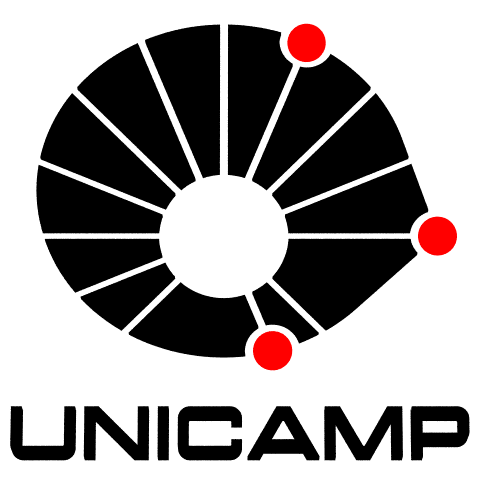
\includegraphics[width=1.5cm]{unicamp}
%        \label{fig:unicamp}
    \end{subfigure}
    \hfill
    % FEEC logo
    \begin{subfigure}{0.45\textwidth}
        \centering
        
\includegraphics[width=1.5cm]{feec}
%        \label{fig:feec}
    \end{subfigure}
\end{figure}

\title{EFC2 - Exercise 2}
\author{Rafael Claro Ito (R.A.: 118430)}
%R.A.: 118430
%ito.rafael@gmail.com
\date{October 2019}
\maketitle
\newpage

%=================================================
\section{Source files}
%=================================================

\paragraph{All code cited and all figures showed here can be found at the following GitHub repository:\\
\url{https://github.com/ito-rafael/IA006C-MachineLearning/tree/master/efc2}\\
In this repository, one can found the following files:\\}

\begin{itemize}
    \item Jupyter Notebook
    \begin{itemize}
        \item \href{https://github.com/ito-rafael/IA006C-MachineLearning/blob/master/efc2/efc2_pre-ex1.ipynb}{efc2\_pre-ex1.ipynb}
        \item \href{https://github.com/ito-rafael/IA006C-MachineLearning/blob/master/efc2/efc2_ex1_binary_classification.ipynb}{efc2\_ex1\_binary\_classification.ipynb}
        \item \href{https://github.com/ito-rafael/IA006C-MachineLearning/blob/master/efc2/efc2_ex2_multiclass_classification.ipynb}{efc2\_ex2\_multiclass\_classification.ipynb}
        \item \href{https://github.com/ito-rafael/IA006C-MachineLearning/blob/master/efc2/efc2_ex2_knn.ipynb}{efc2\_ex2\_knn.ipynb}
    \end{itemize}
    \item \LaTeX
    \begin{itemize}
        \item \href{https://github.com/ito-rafael/IA006C-MachineLearning/blob/master/efc2/LaTeX/efc2.tex}{efc2.tex}
    \end{itemize}
\end{itemize}

\paragraph{The notebook ``efc2\_pre-ex1'' plots the histograms for the exercise 1 and it is used for data visualization. It shows the input features histograms for the raw data and after a data standardization. Also, it shows the correlation between these data.}

\paragraph{The notebook ``efc2\_ex1\_binary\_classification'' effectively implements the logistic regression used to perform a binary classification proposed in exercise 1.}

\paragraph{The notebooks ``efc2\_ex2\_multiclass\_classification'' and ``efc2\_ex2\_knn'' implements the algorithms to perform a multiclass classification proposed in exercise 2. The former one uses the softmax approach while the latter one implements the K-Nearest Neighbors (kNN) algorithm.}

\bigskip

%=================================================
\section{Part 1 - Binary Classification}
%=================================================

%=======================================
\subsection{a) Input features characteristics analysis considering the histograms and correlation measures between them.}
%=======================================

\paragraph{The first thing we did for this item, was to plot the histograms of the data before and after standardization. The histograms for the raw data can be seen in Figure \ref{fig:pre-ex1-raw_histograms} and the histograms for the standardized data can be seen in Figure \ref{fig:pre-ex1-std_histograms}. To perform the standardization, the StandardScaler class provided by the scikit-learn library was used.}

\paragraph{Figure \ref{fig:pre-ex1-sbs_histograms} shows the histograms of the input features separated according to the labels. The orange plot represents the label 0 (female class) and the blue plot represents the label 1 (male class).}

\paragraph{As we can see in Figure \ref{fig:pre-ex1-sbs_histograms}, some features may be visually very informative about the class. For example, features ``mean fun'', ``Q25''  and ``IQR'' can be very informative and show the classes in a distinct way. Features like ``sd'', ``sp ent'', ``smf'' and ``mode'' can bring some information about the class, but they are not so obvious, since both classes are showed in a specific value of the histograms. In some cases, it is not possible to separate the classes only by visually analyzing the histograms of the features in a straightforward way, like in the case of the features ``Q75'', ``maxfun'' or ``modindx'', since the data has values in a similar range bor both classes.}

\newpage
% histograms of raw features

\begin{figure}[H]
    \centering
    % sd
    \begin{subfigure}{0.32\textwidth}
        \centering
        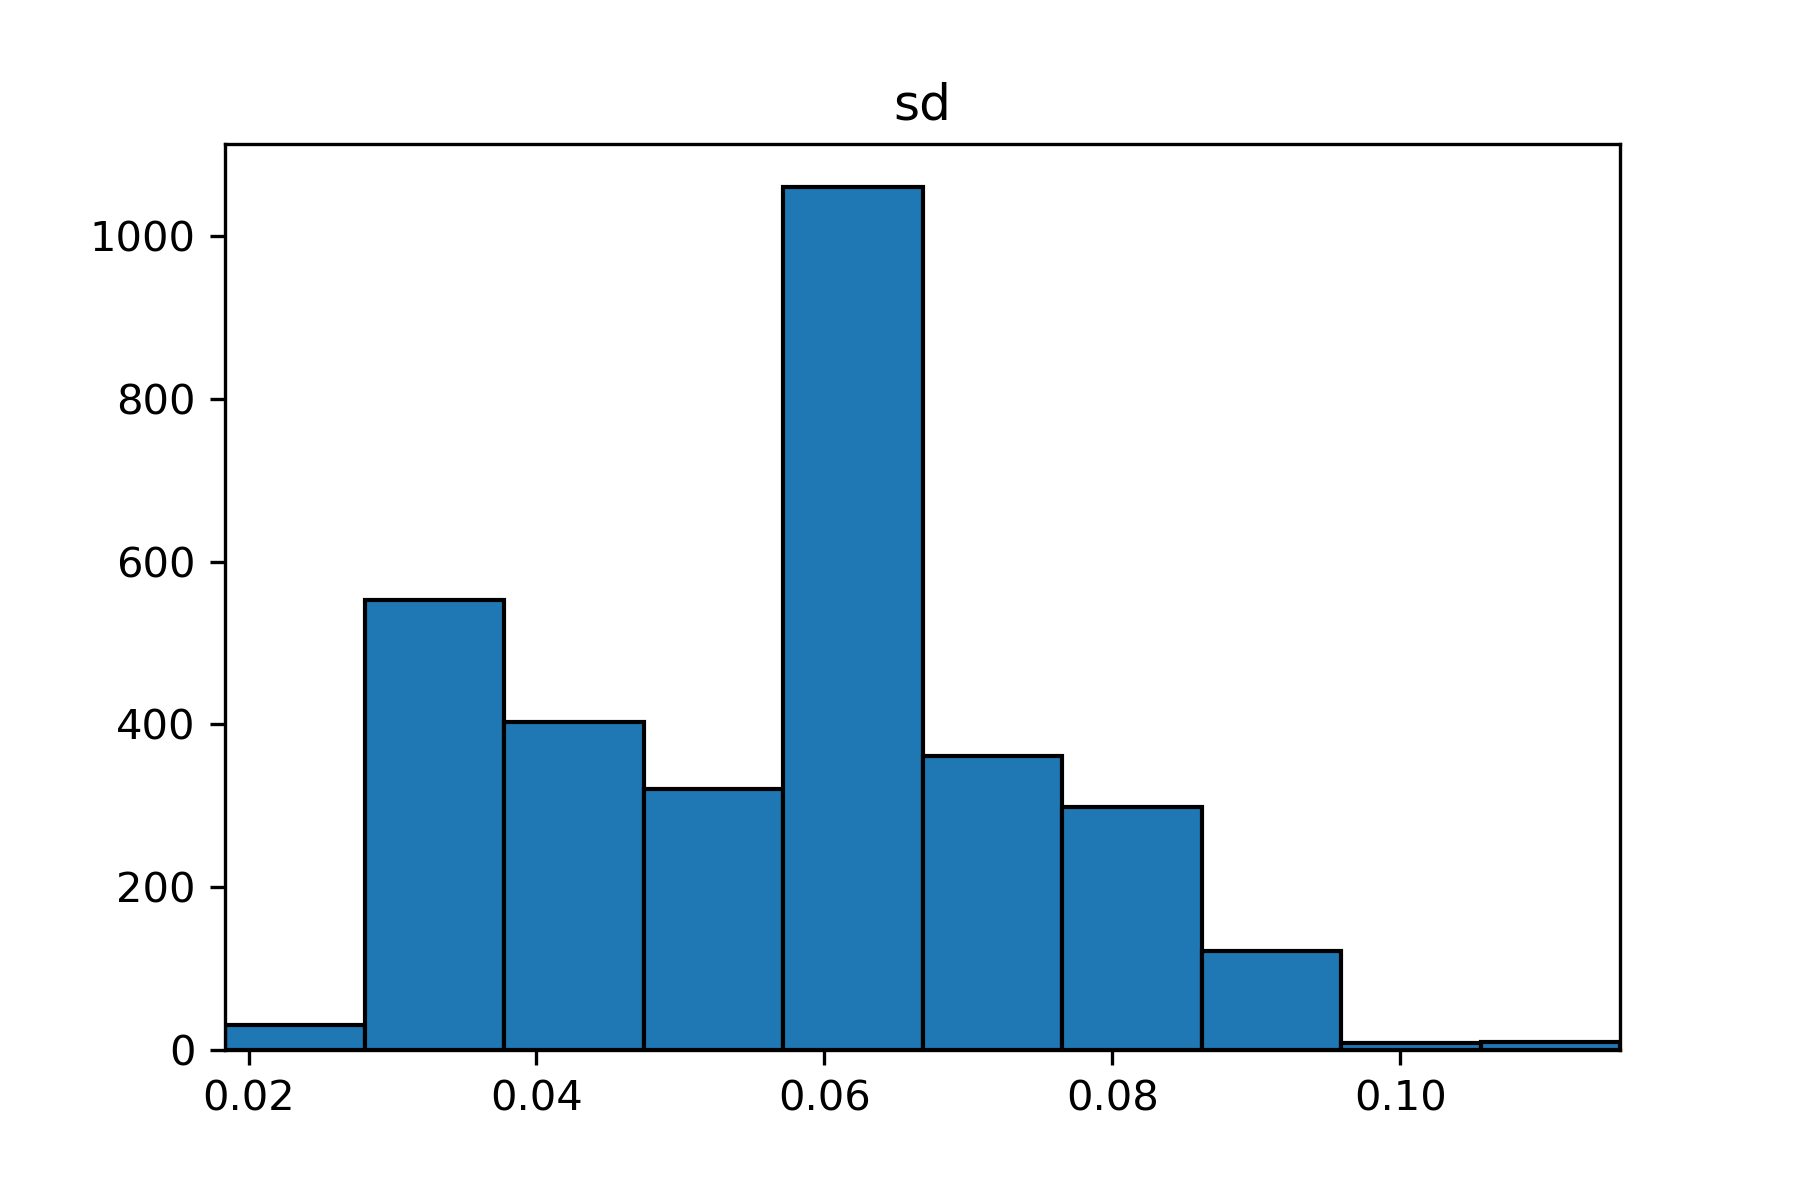
\includegraphics[width=3.85cm]{raw_0_sd}
        \caption{sd}
        \label{fig:sub_raw_1}
    \end{subfigure}
    \hfill
    % median
    \begin{subfigure}{0.32\textwidth}
        \centering
        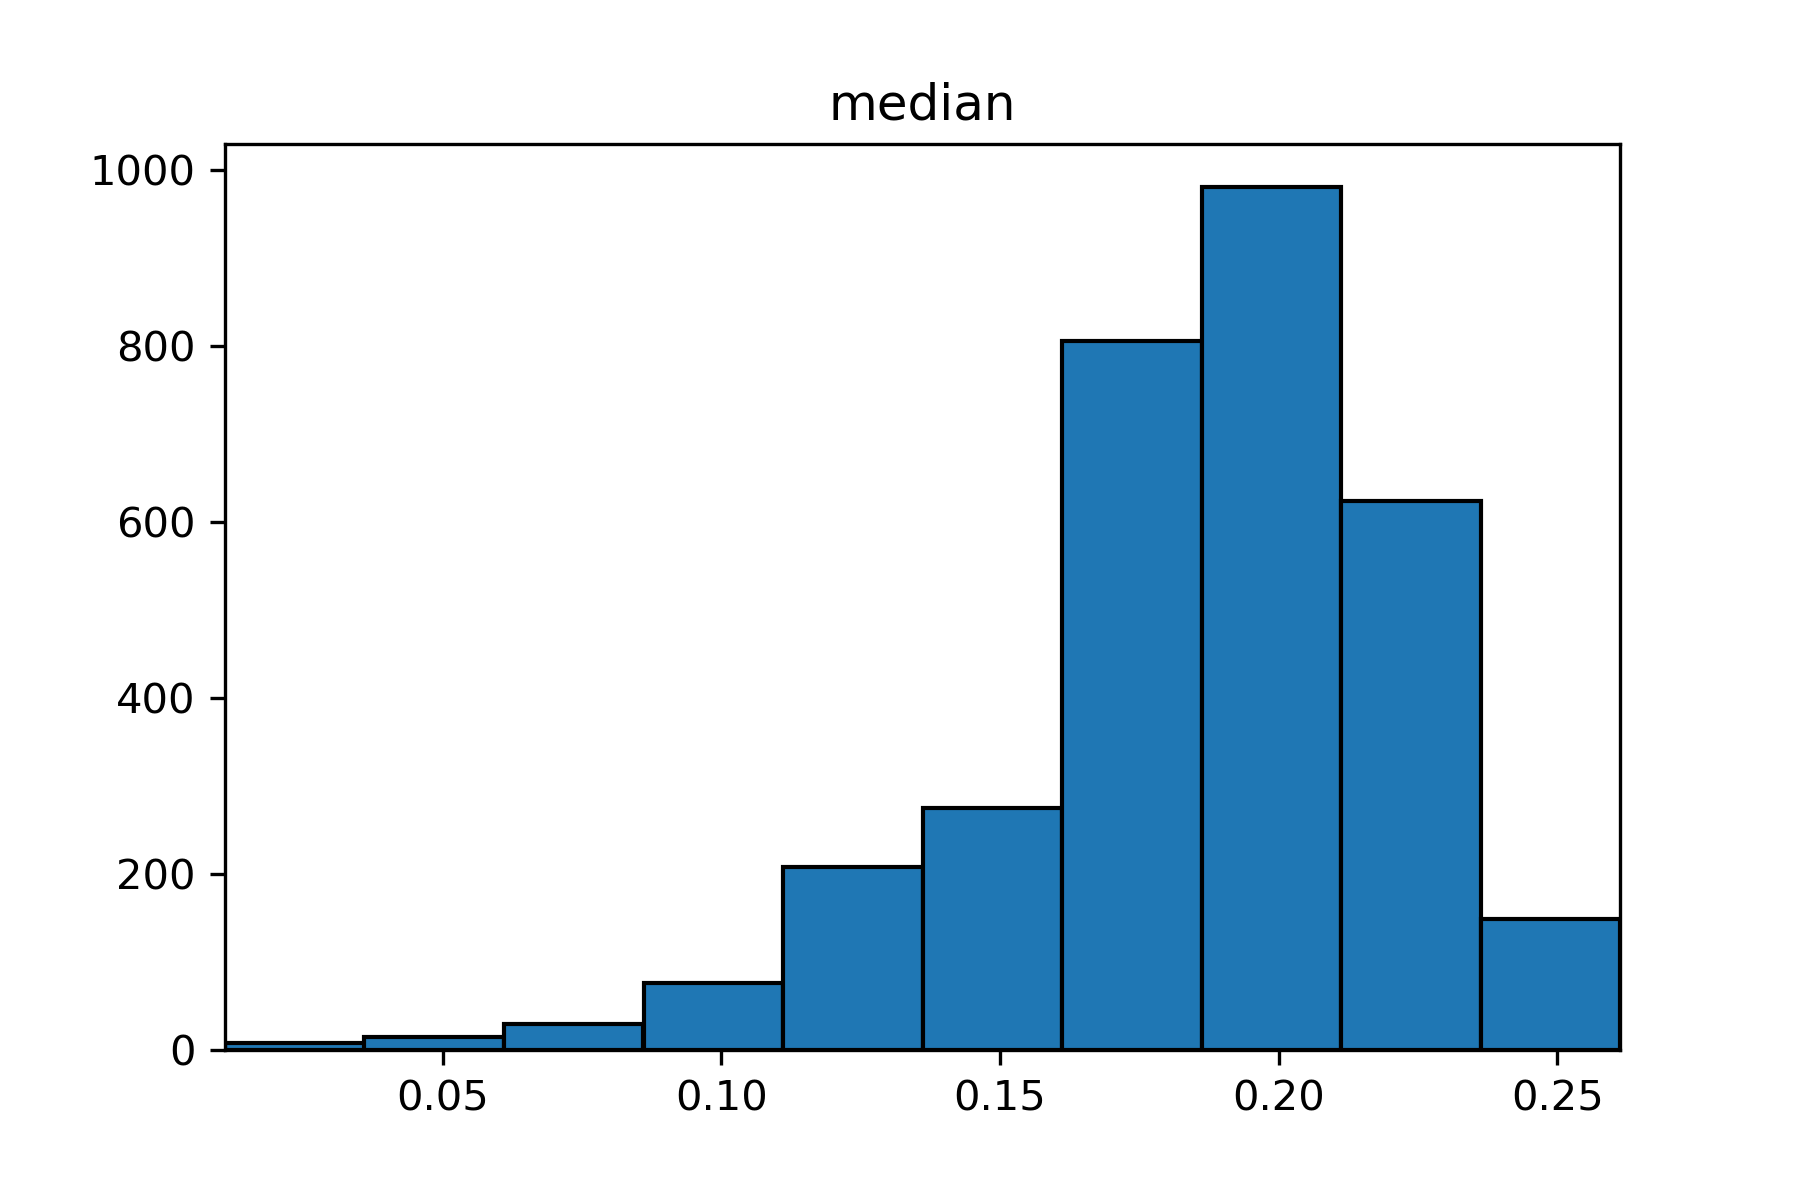
\includegraphics[width=3.85cm]{raw_1_median}
        \caption{median}
        \label{fig:sub_raw_2}
    \end{subfigure}
    \hfill
    % Q25
    \begin{subfigure}{0.32\textwidth}
        \centering
        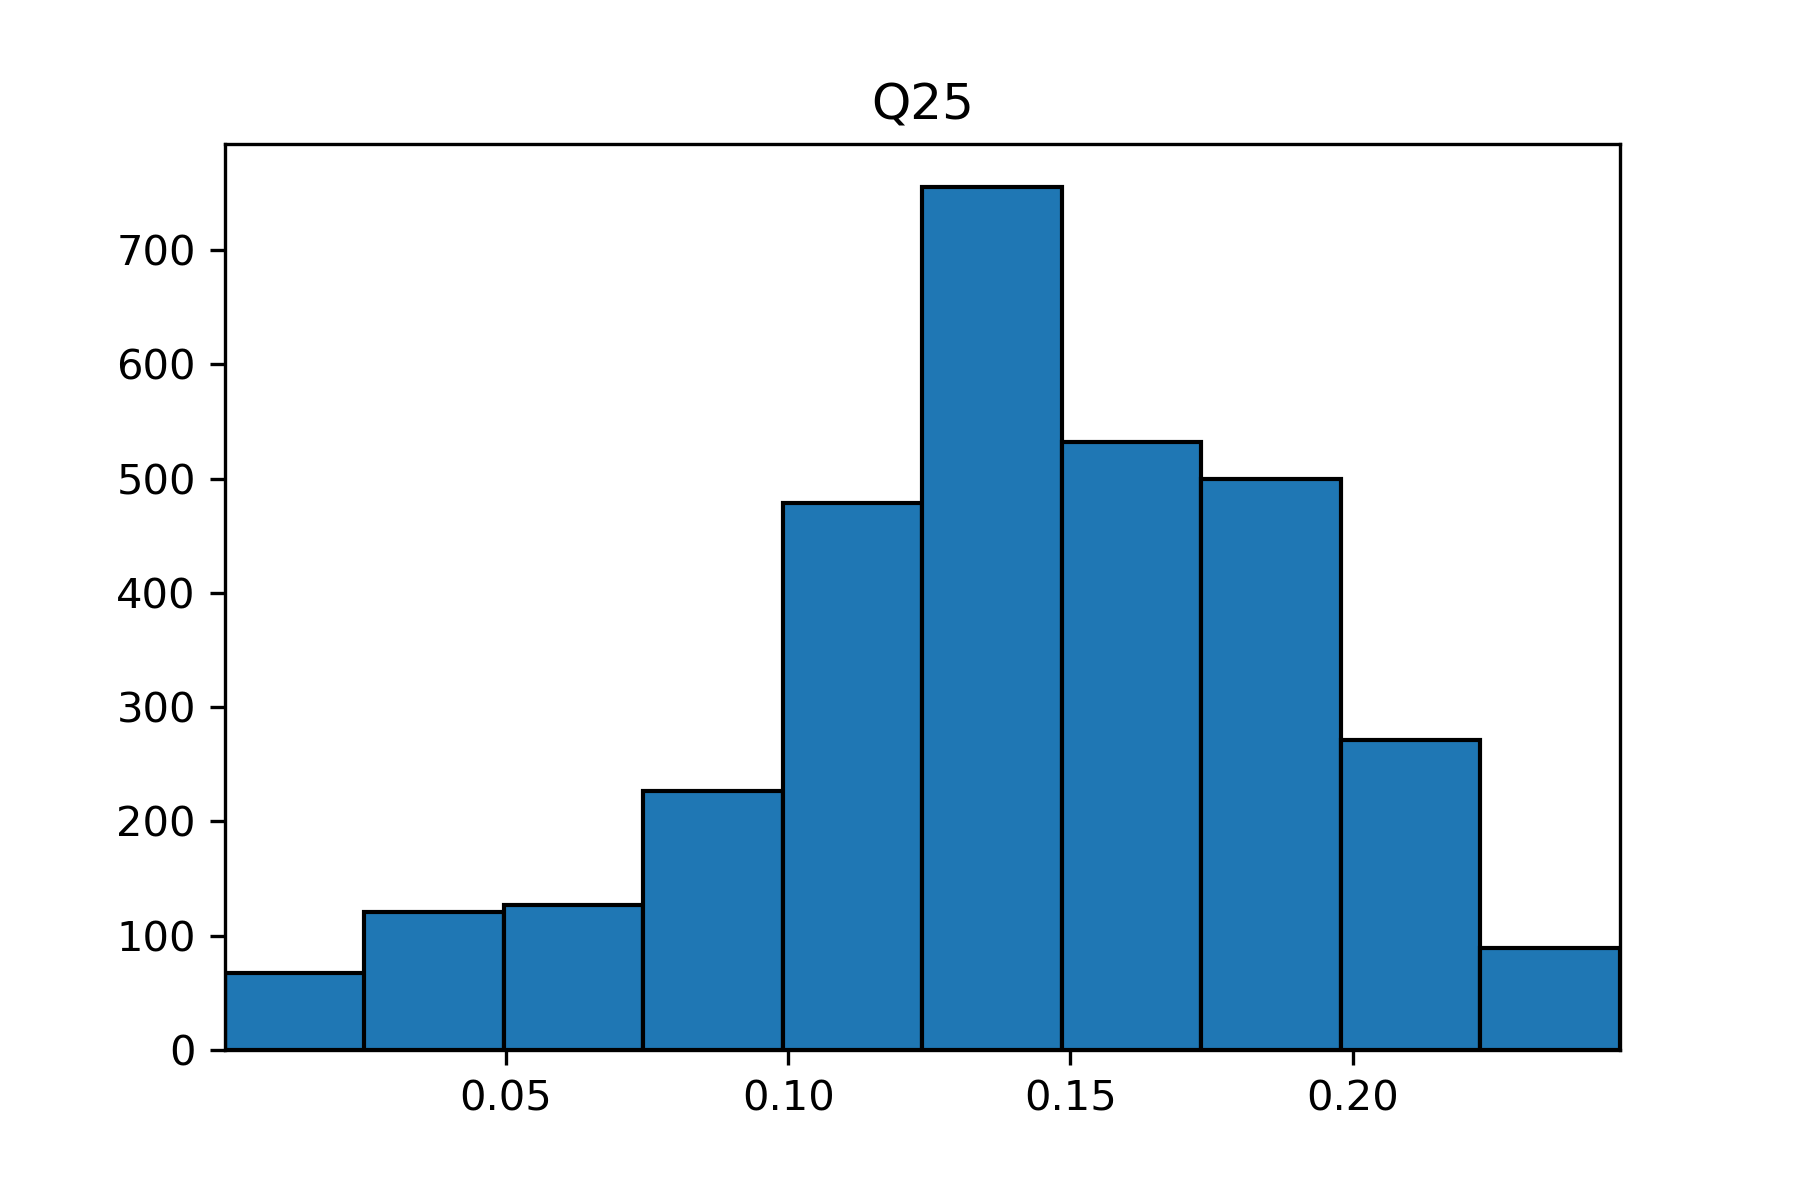
\includegraphics[width=3.85cm]{raw_2_Q25}
        \caption{Q25}
        \label{fig:sub_raw_3}
    \end{subfigure}%
    \\
    % Q75
    \begin{subfigure}{0.32\textwidth}
        \centering
        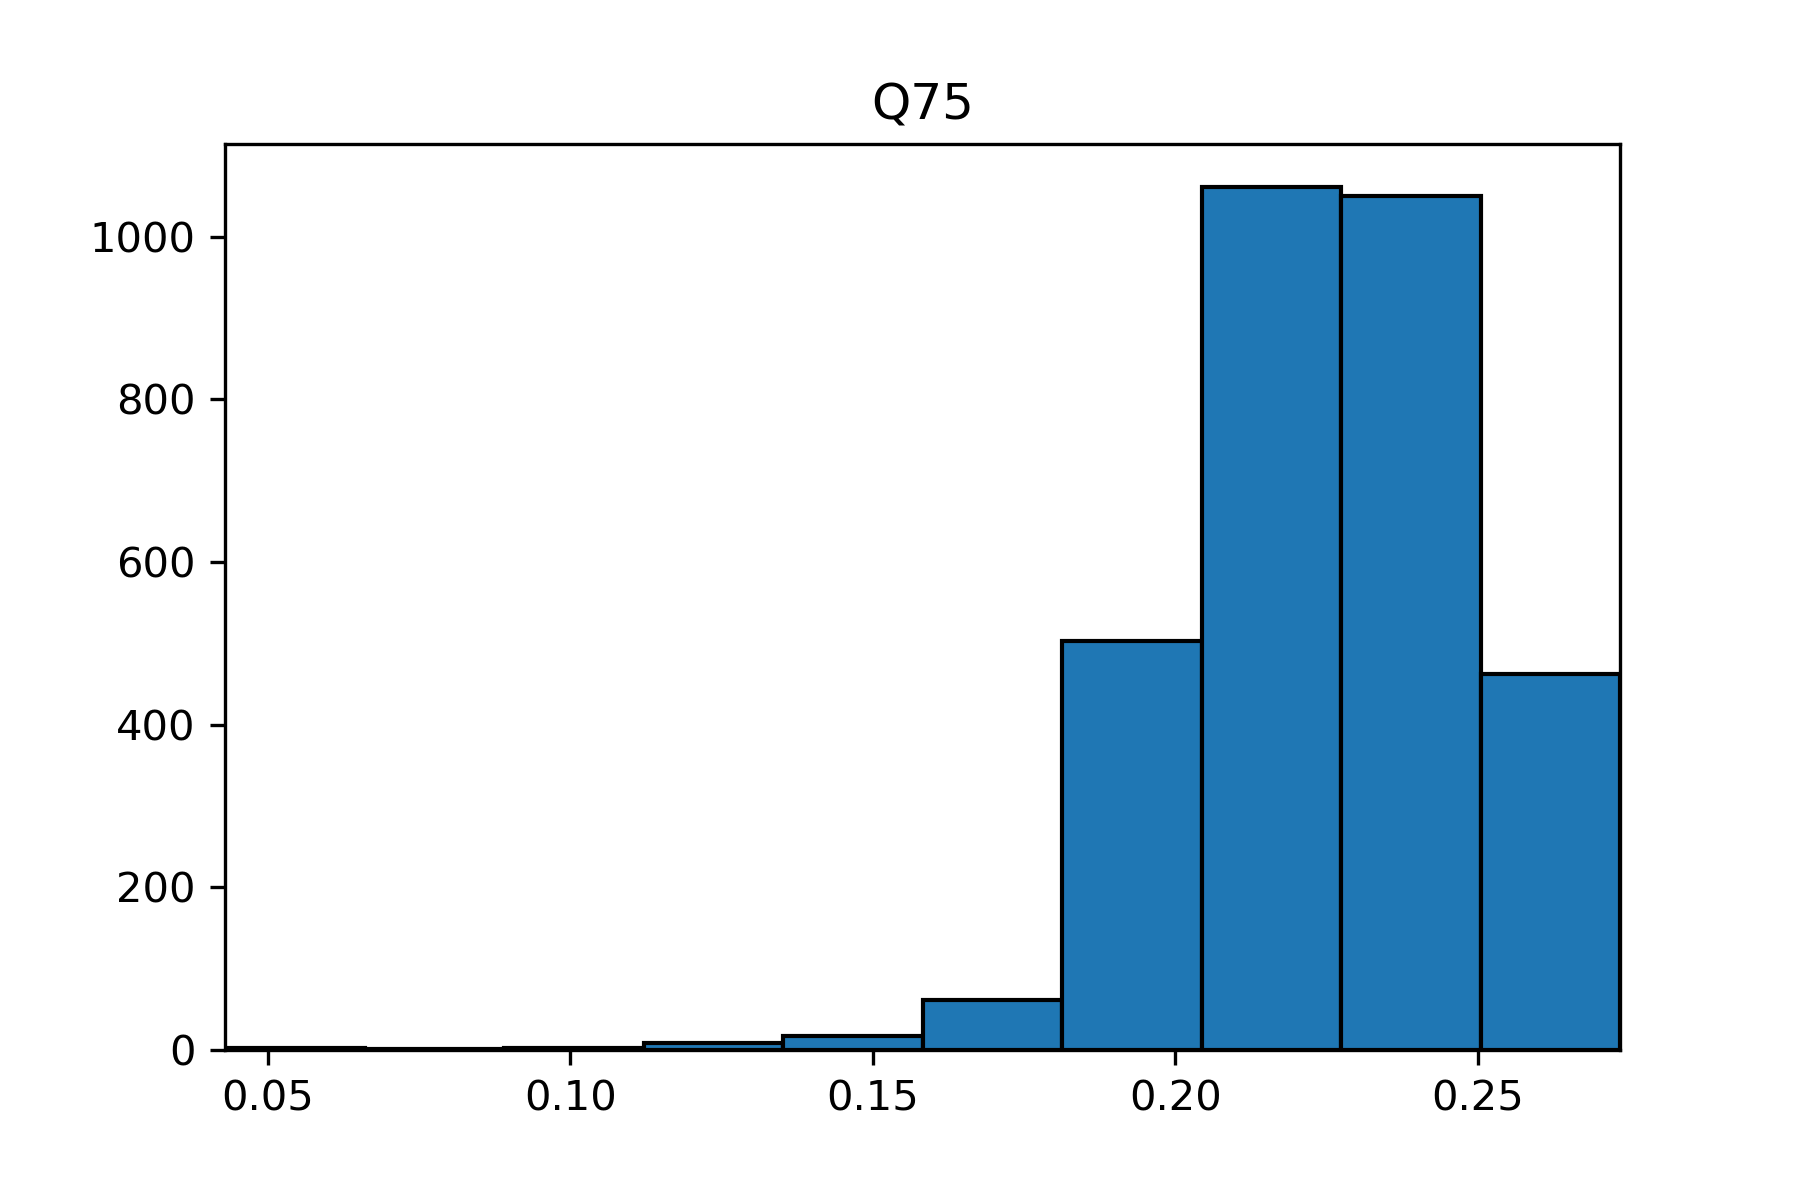
\includegraphics[width=3.85cm]{raw_3_Q75}
        \caption{Q75}
        \label{fig:sub_raw_4}
    \end{subfigure}\hfill
    % Q75
    \begin{subfigure}{0.32\textwidth}
        \centering
        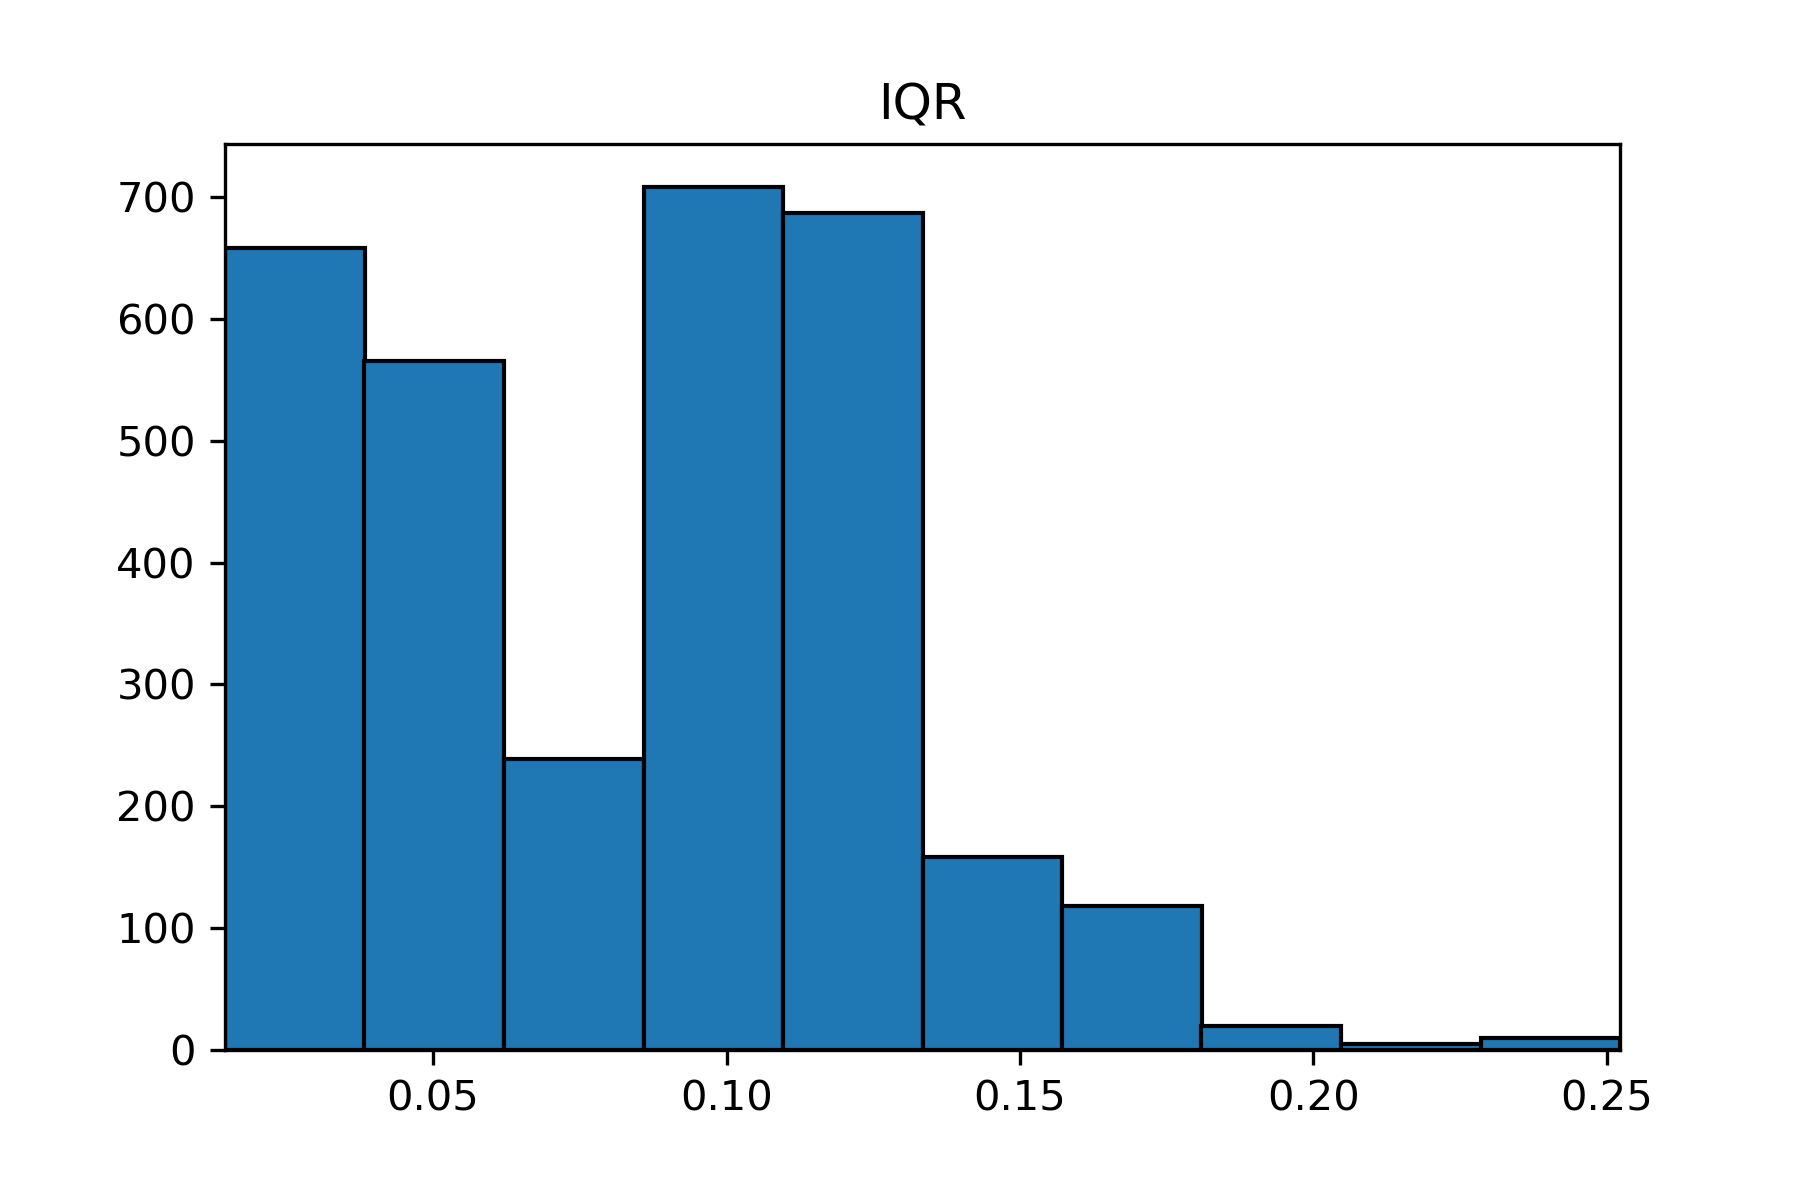
\includegraphics[width=3.85cm]{raw_4_IQR}
        \caption{IQR}
        \label{fig:sub_raw_5}
    \end{subfigure}\hfill
    % skew
    \begin{subfigure}{0.32\textwidth}
        \centering
        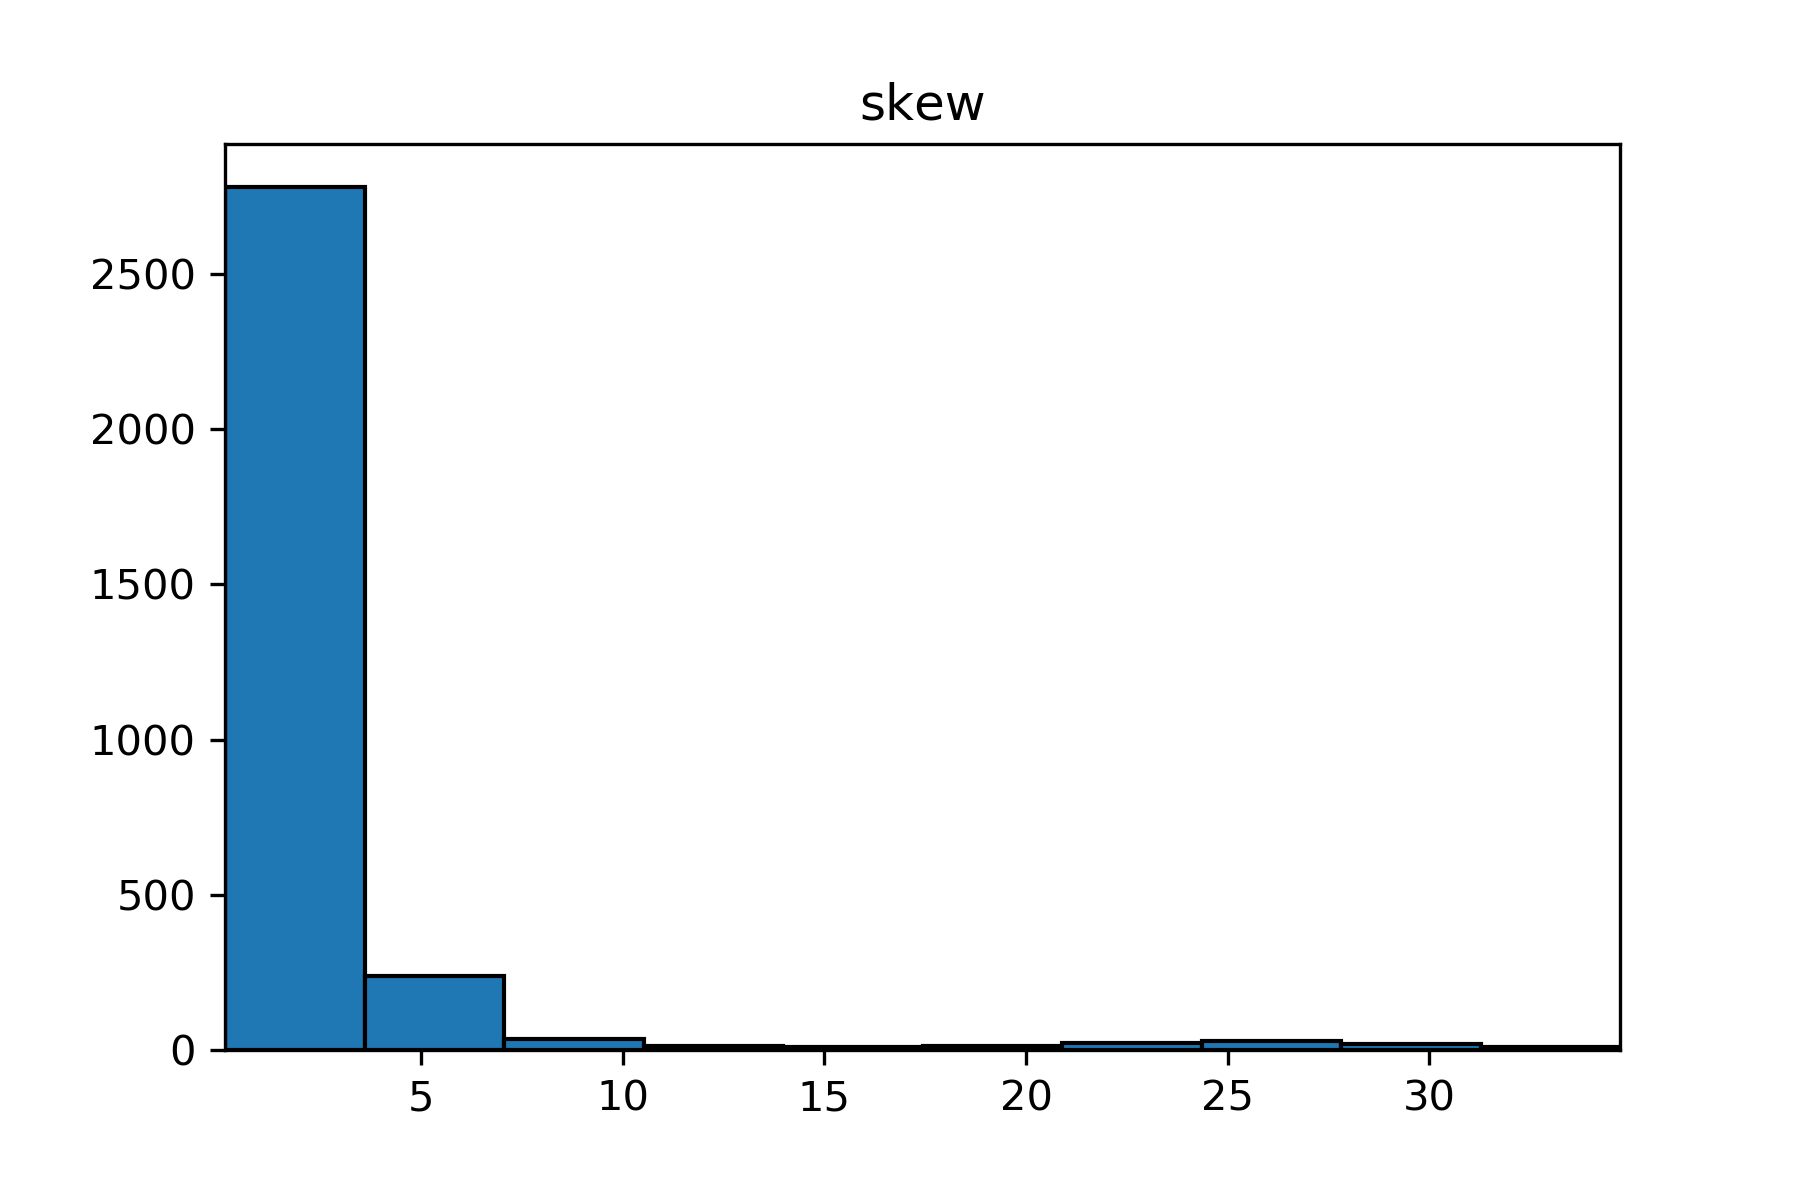
\includegraphics[width=3.85cm]{raw_5_skew}
        \caption{skew}
        \label{fig:sub_raw_6}
    \end{subfigure}
    \\
    % kurt
    \begin{subfigure}{0.32\textwidth}
        \centering
        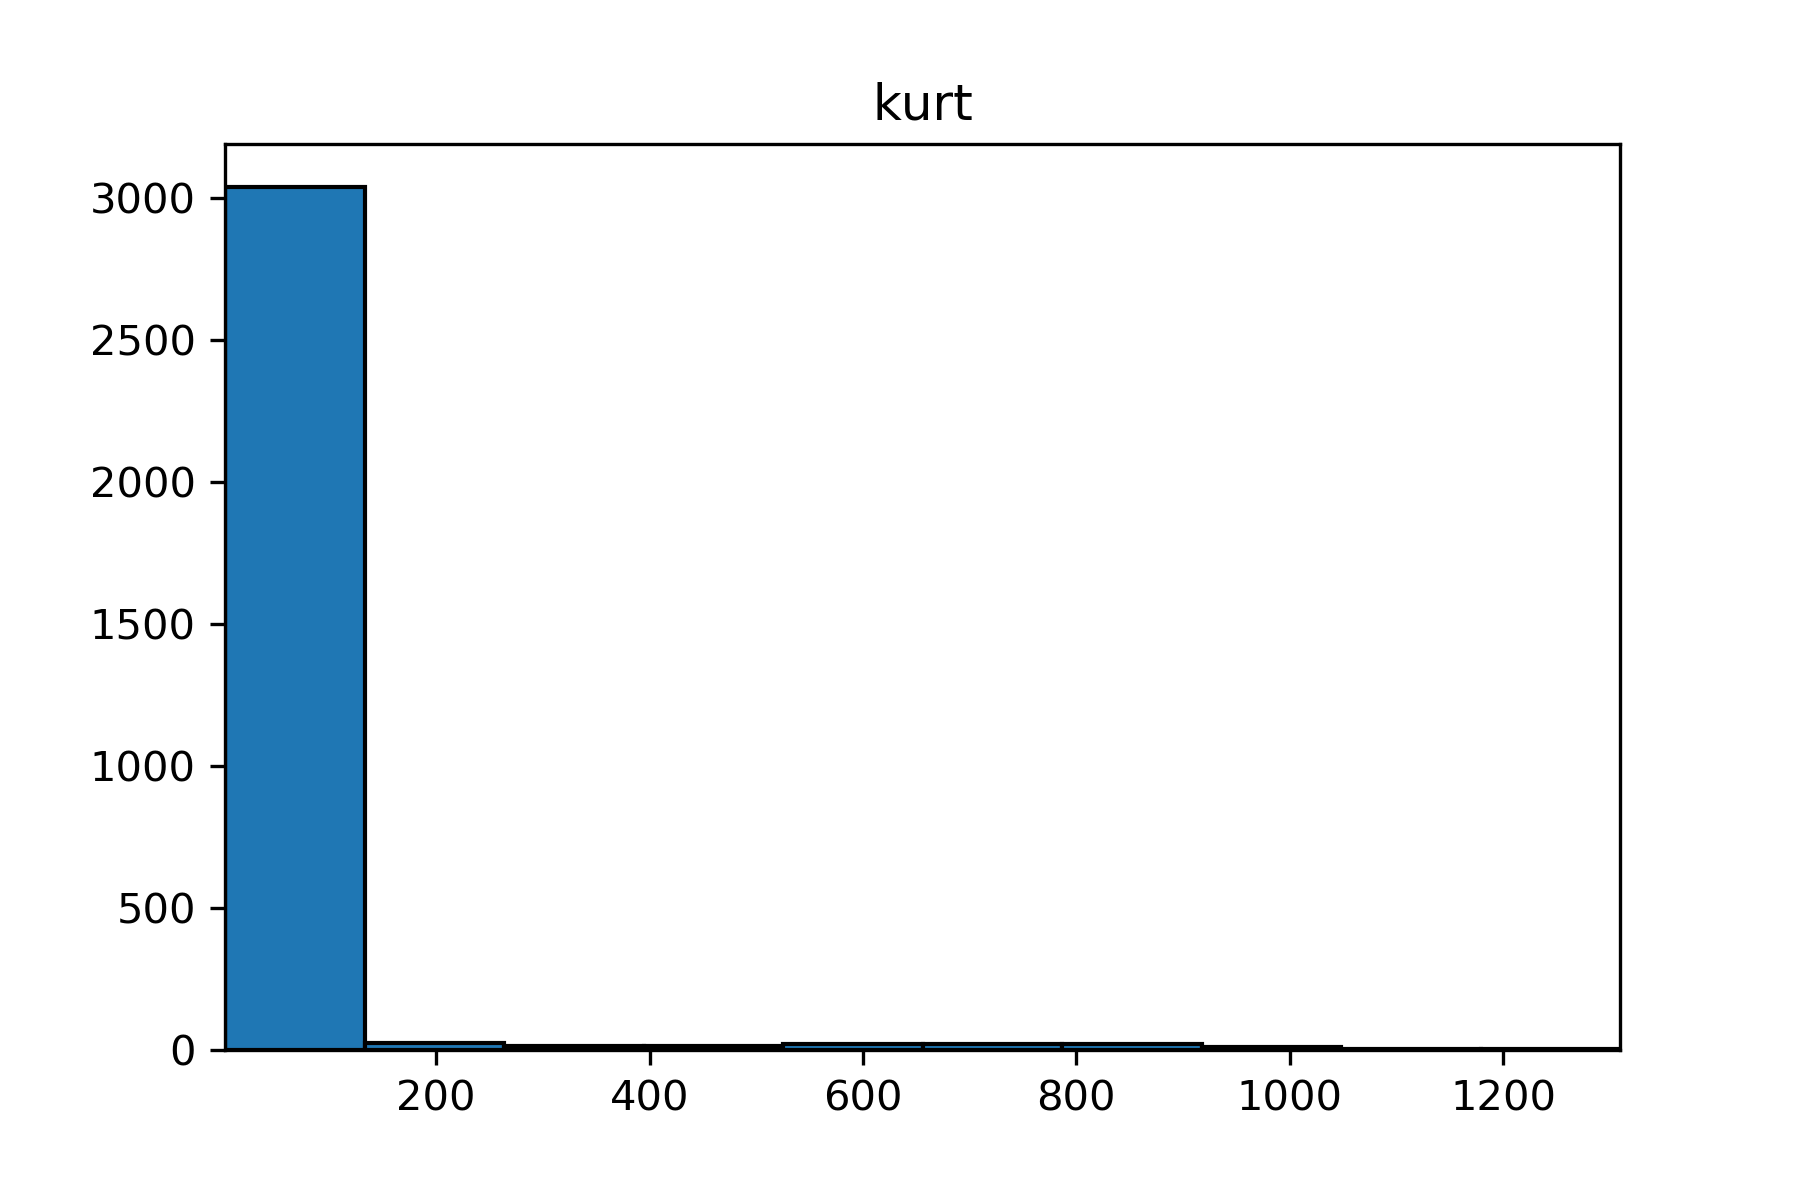
\includegraphics[width=3.85cm]{raw_6_kurt}
        \caption{kurt}
        \label{fig:sub_raw_7}
    \end{subfigure}\hfill
    % sp ent
    \begin{subfigure}{0.32\textwidth}
        \centering
        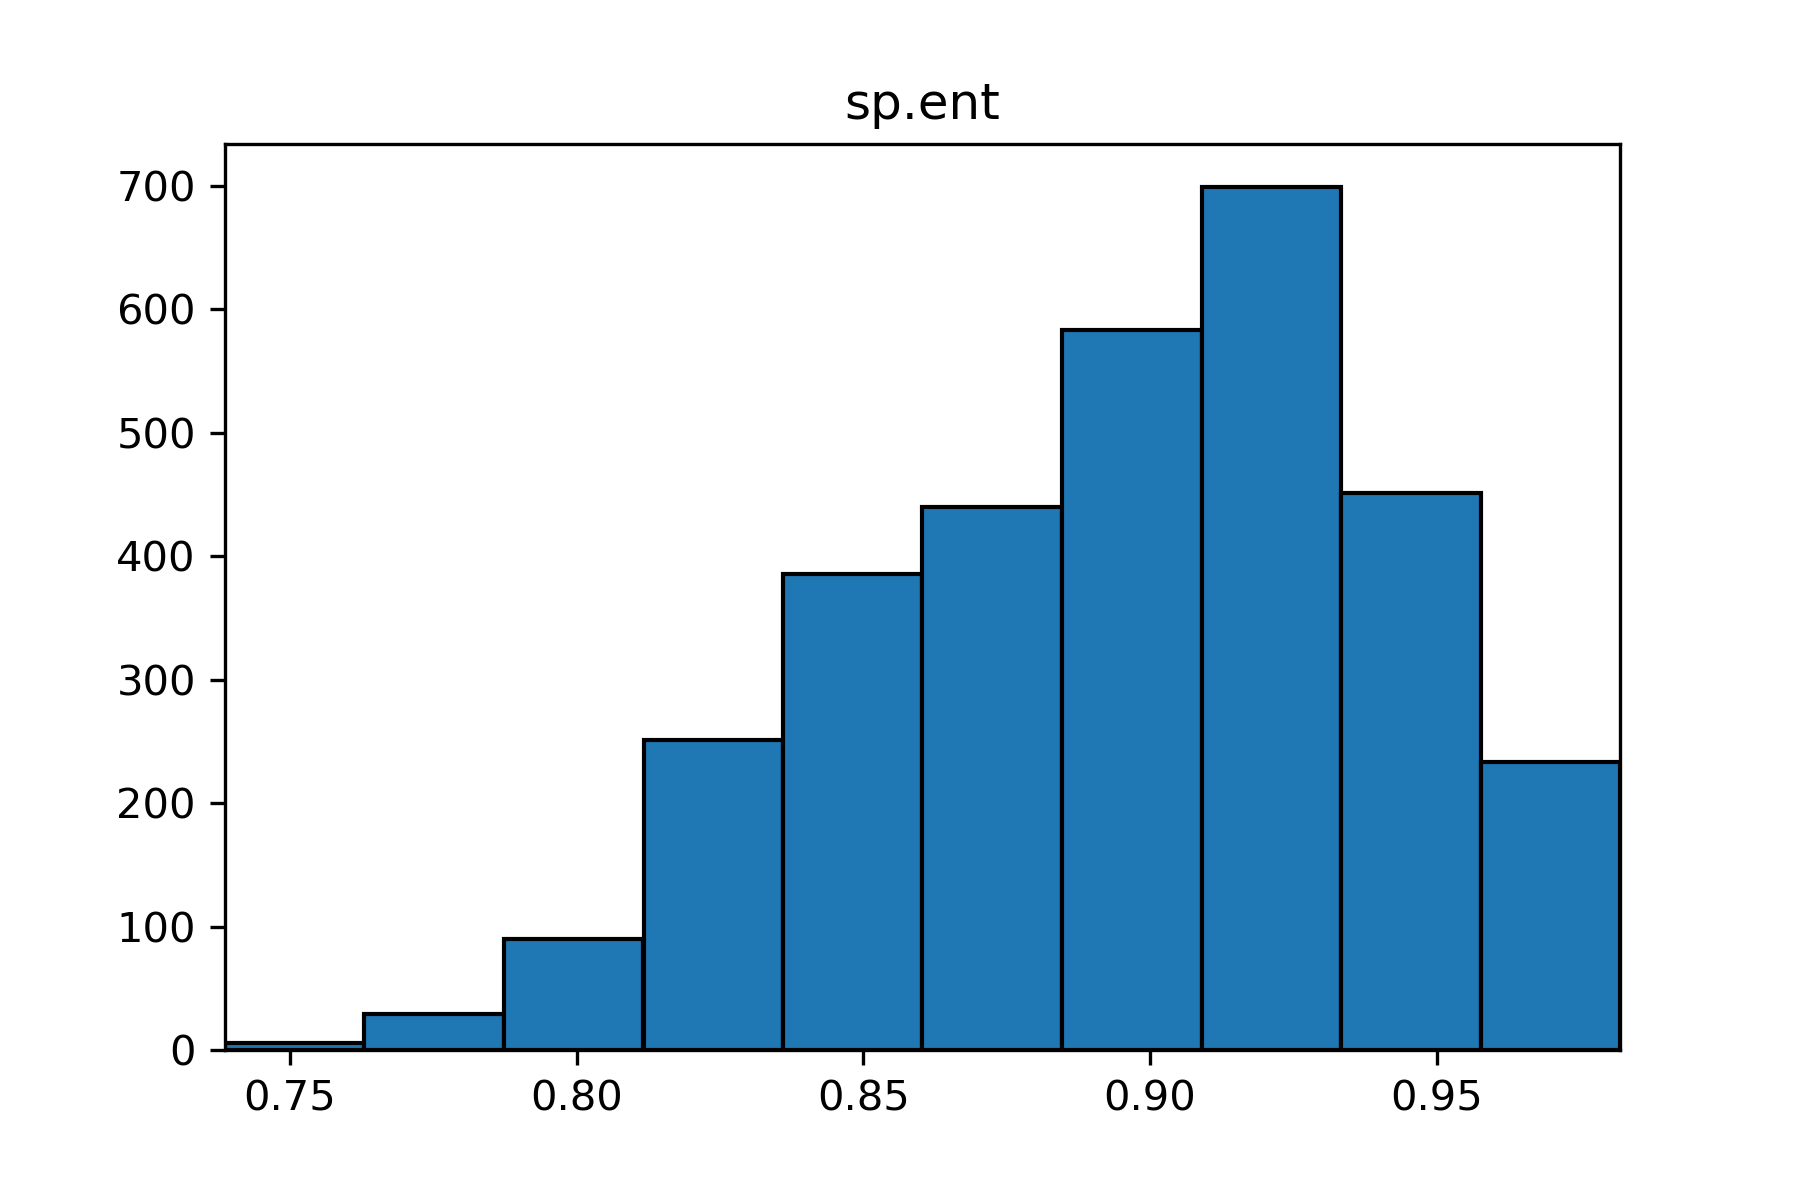
\includegraphics[width=3.85cm]{raw_7_sp_ent}
        \caption{sp ent}
        \label{fig:sub_raw_8}
    \end{subfigure}\hfill
    % sfm
    \begin{subfigure}{0.32\textwidth}
        \centering
        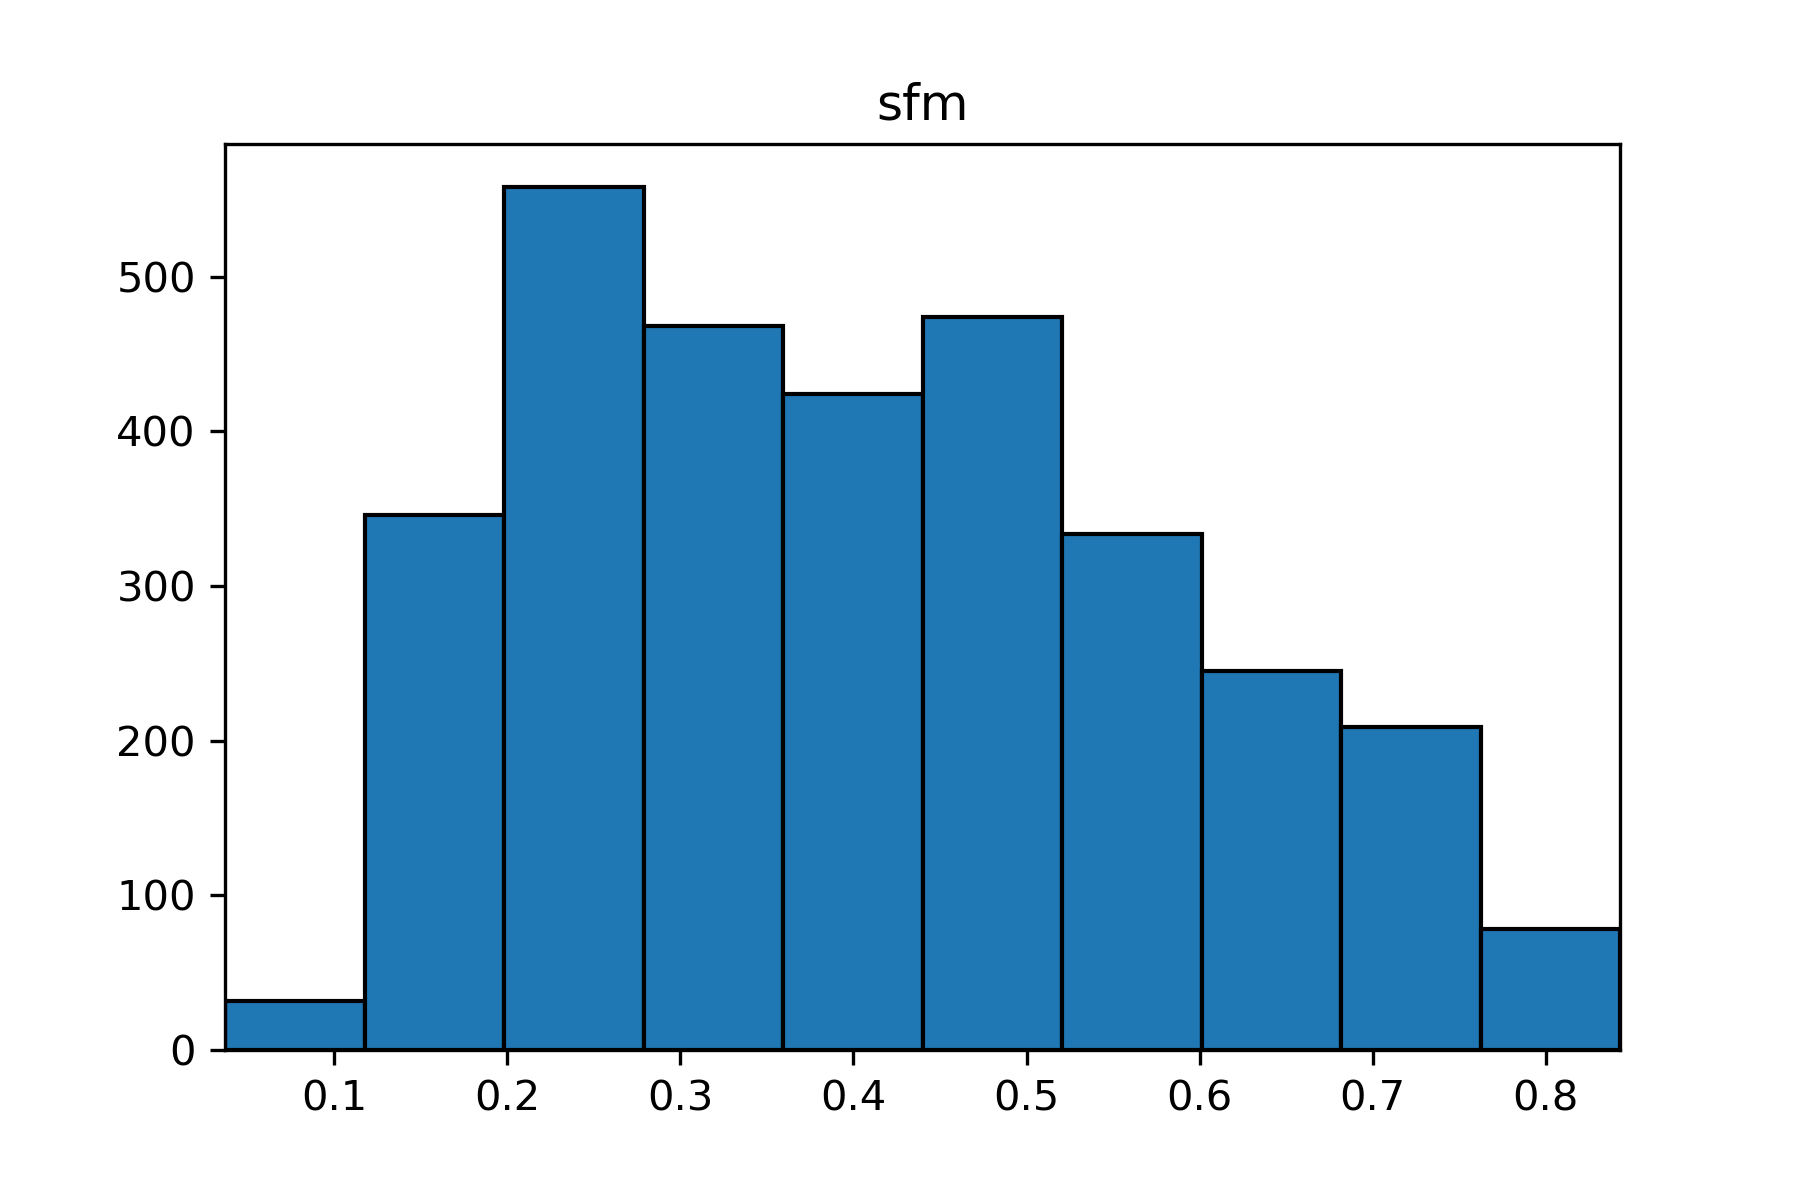
\includegraphics[width=3.85cm]{raw_8_sfm}
        \caption{smf}
        \label{fig:sub_raw_9}
    \end{subfigure}\hfill
    % mode
    \begin{subfigure}{0.32\textwidth}
        \centering
        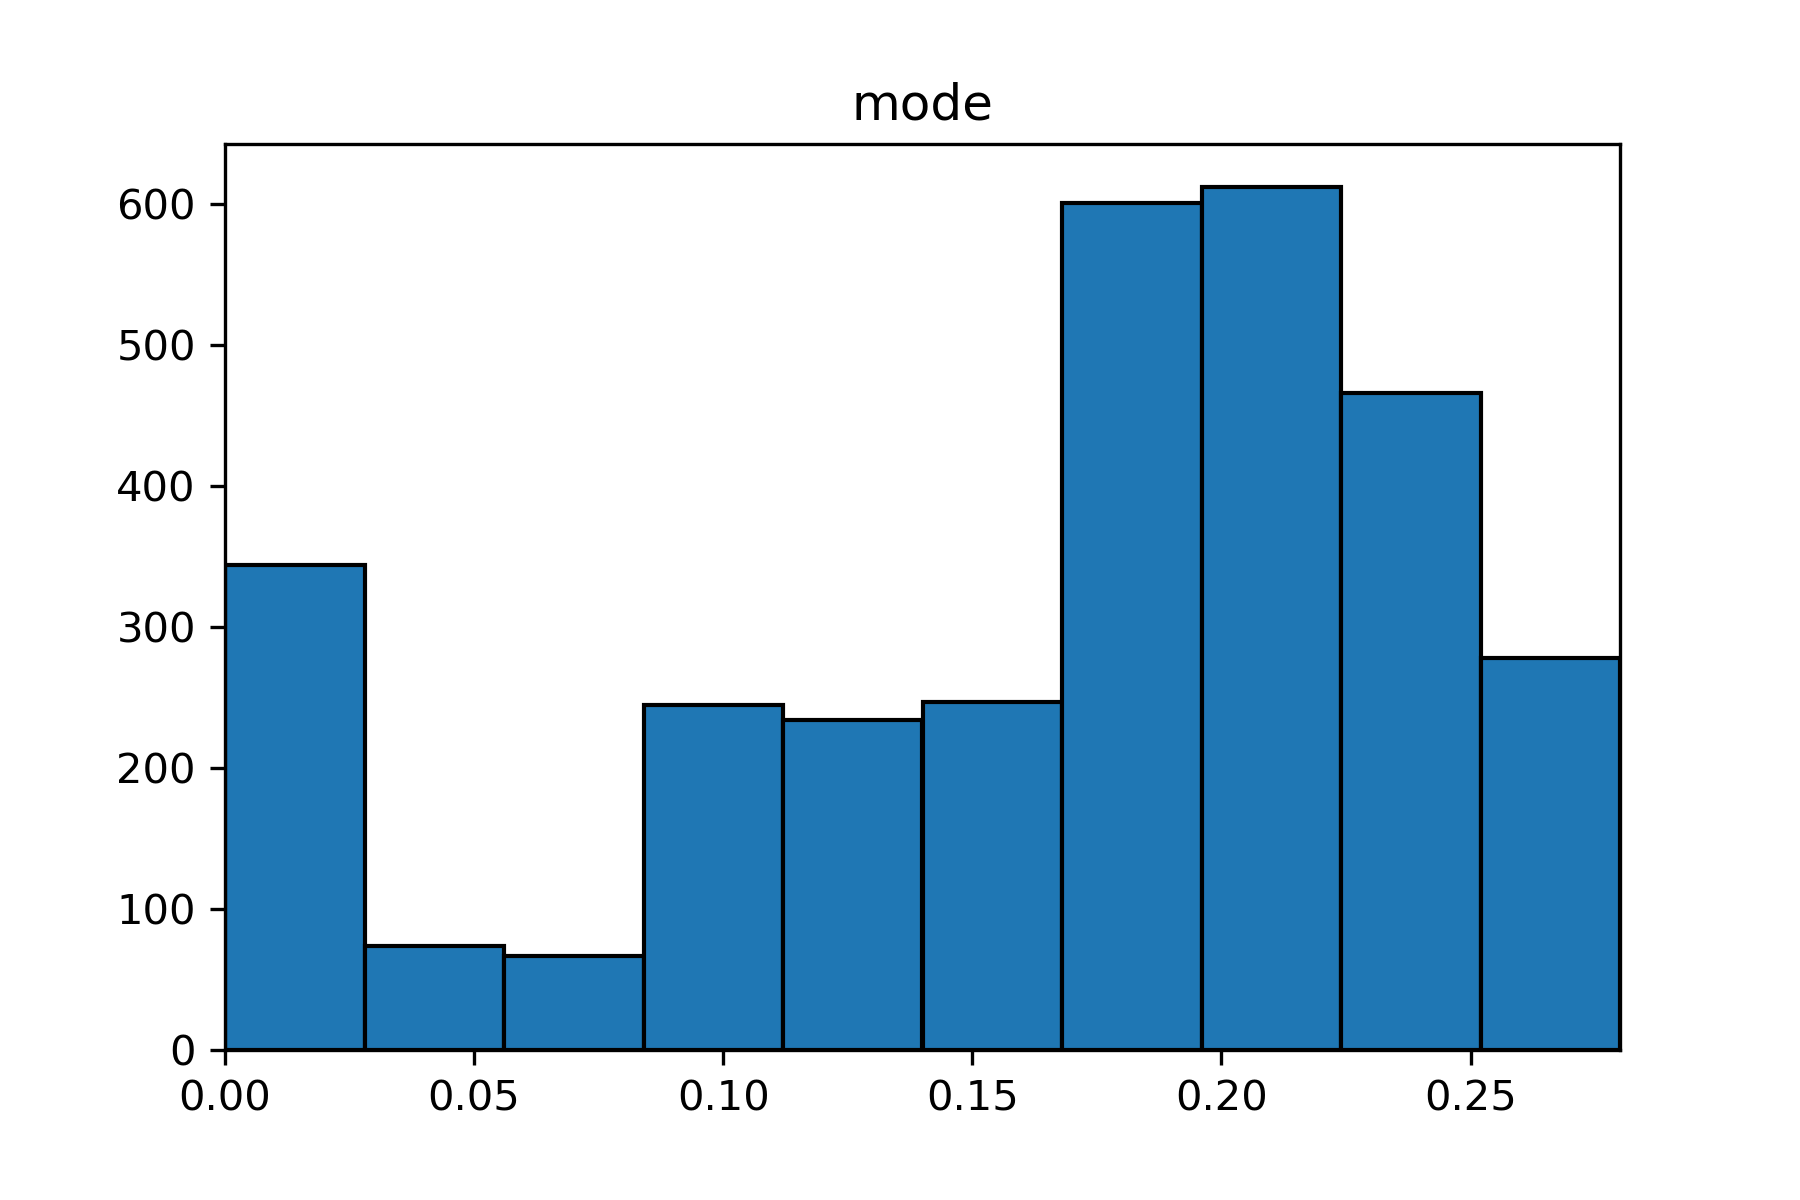
\includegraphics[width=3.85cm]{raw_9_mode}
        \caption{mode}
        \label{fig:sub_raw_10}
    \end{subfigure}\hfill
    % centroid
    \begin{subfigure}{0.32\textwidth}
        \centering
        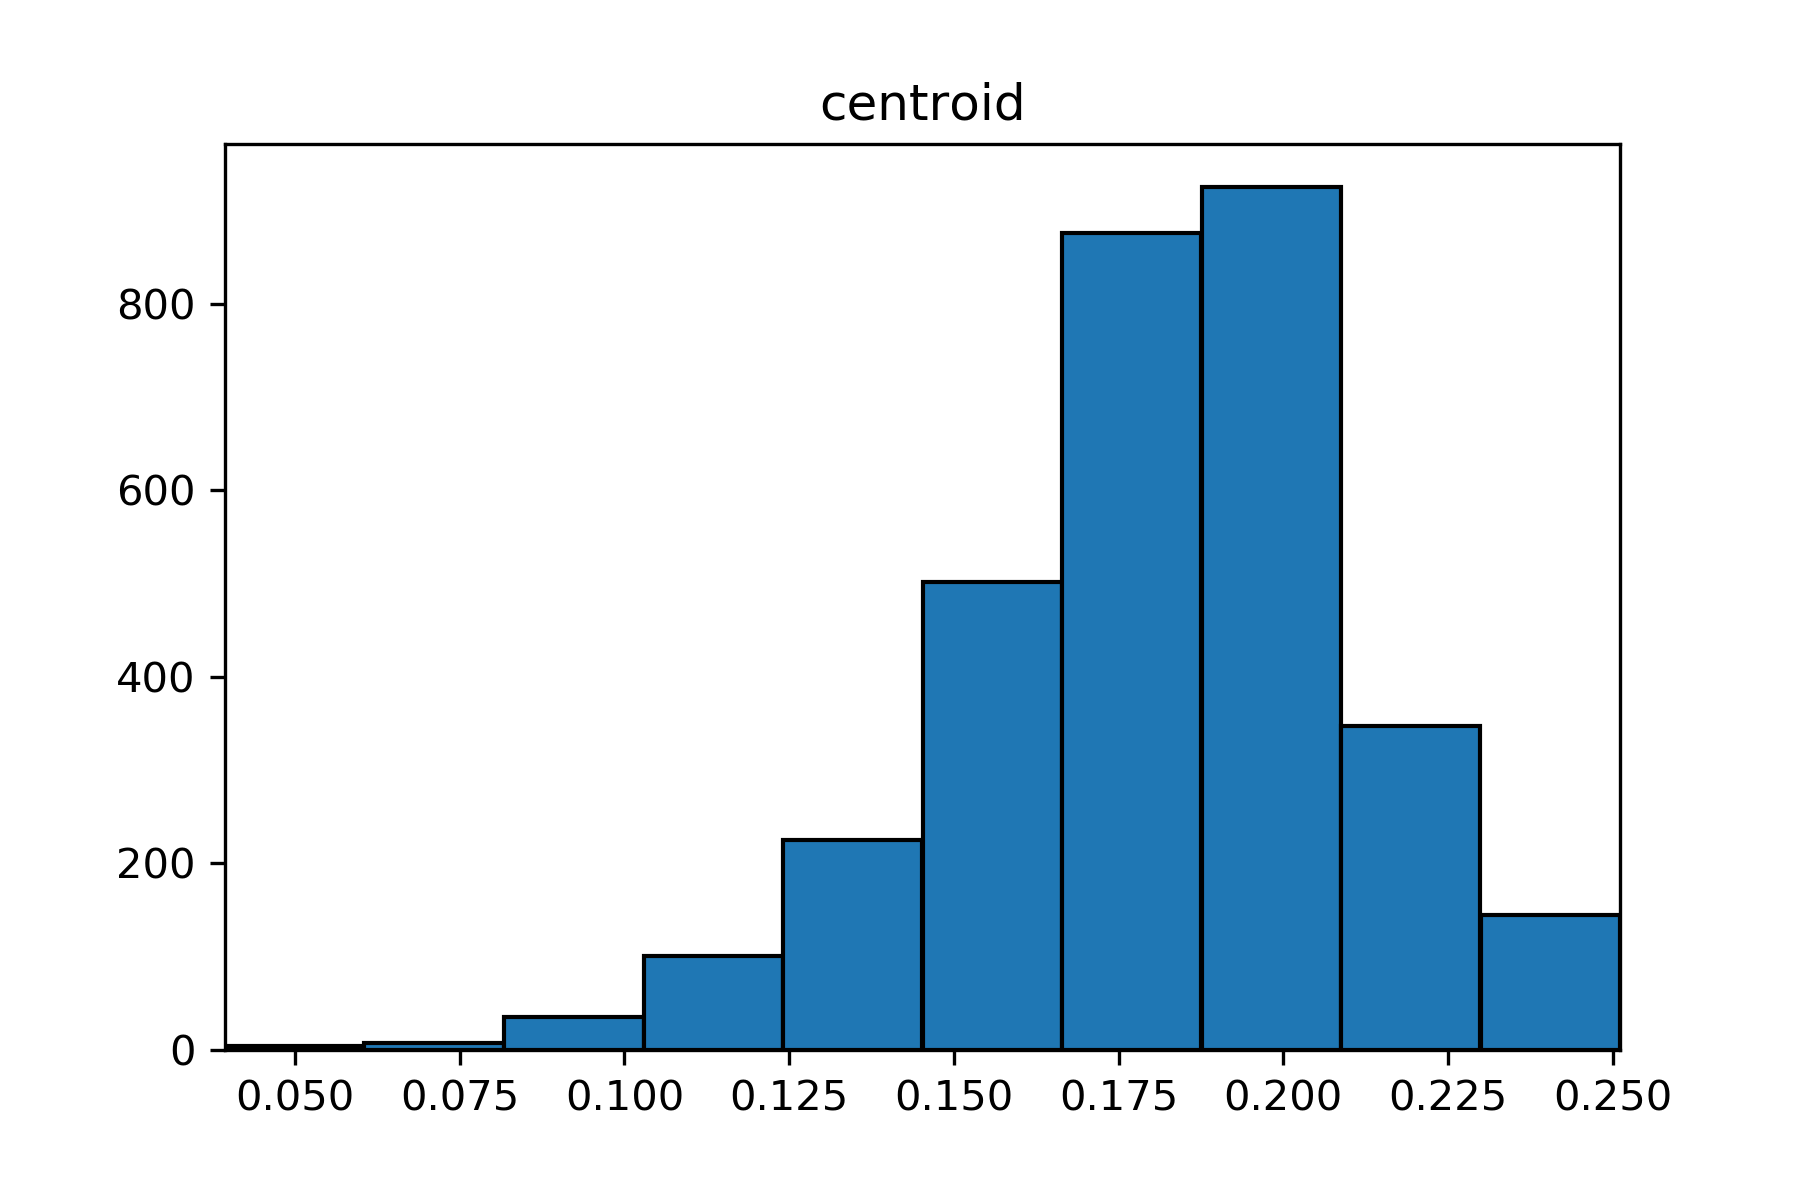
\includegraphics[width=3.85cm]{raw_10_centroid}
        \caption{centroid}
        \label{fig:sub_raw_11}
    \end{subfigure}\hfill
    % meanfun
    \begin{subfigure}{0.32\textwidth}
        \centering
        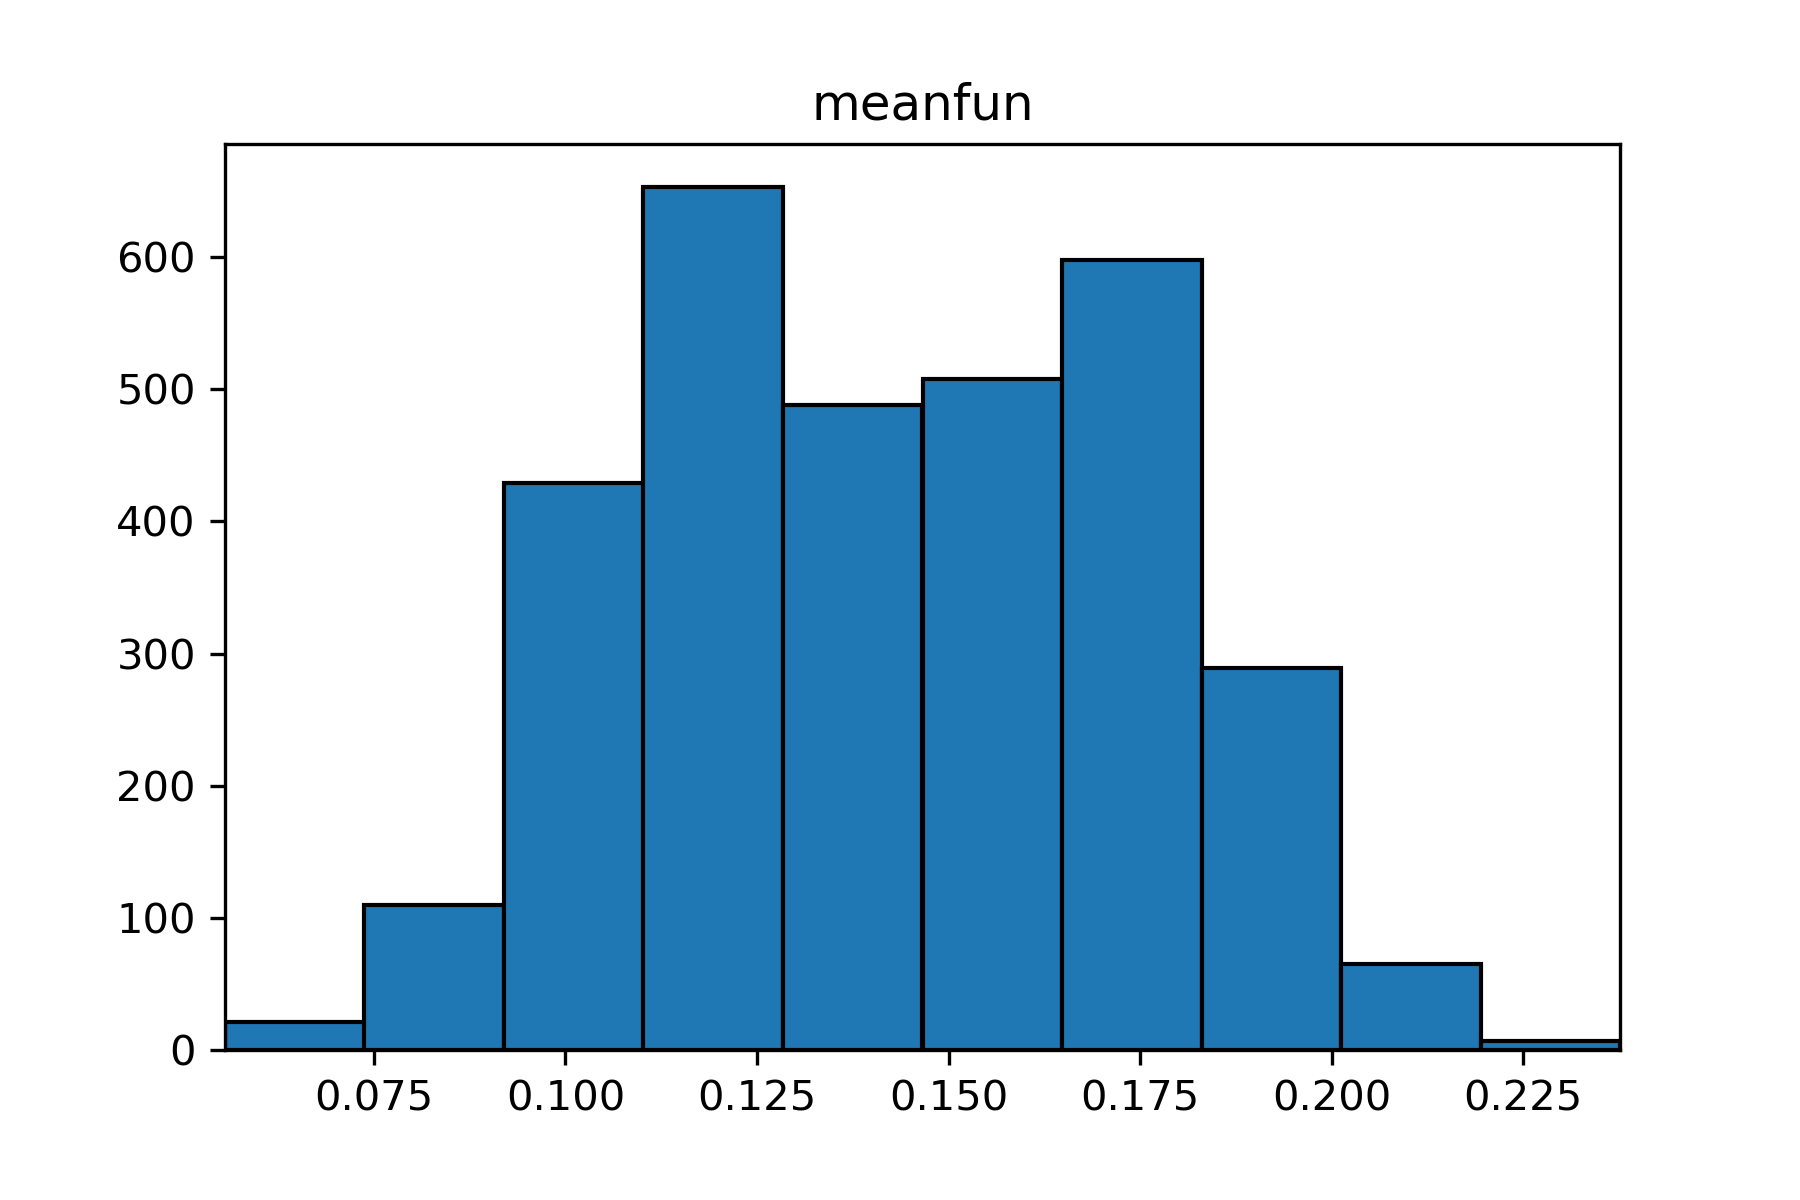
\includegraphics[width=3.85cm]{raw_11_meanfun}
        \caption{meanfun}
        \label{fig:sub_raw_12}
    \end{subfigure}\hfill
    % minfun
    \begin{subfigure}{0.32\textwidth}
        \centering
        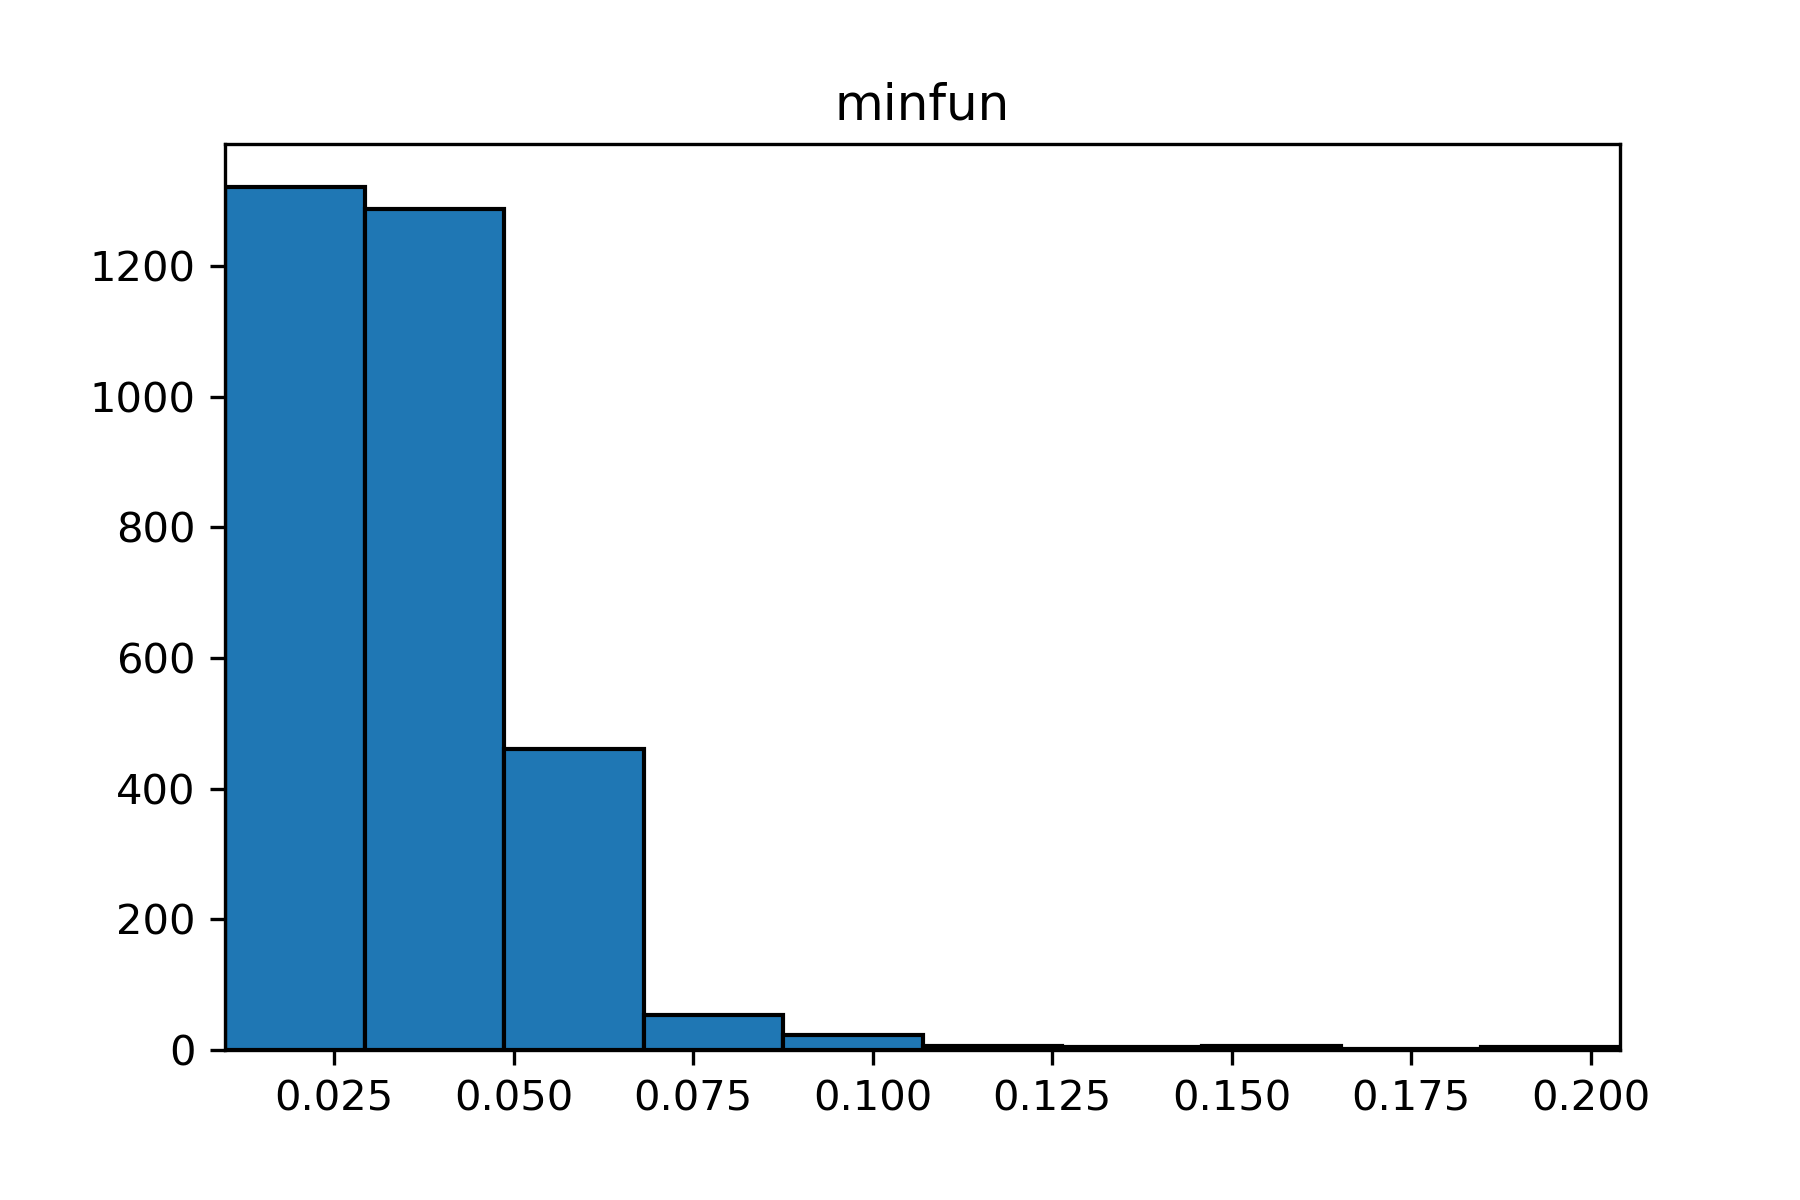
\includegraphics[width=3.85cm]{raw_12_minfun}
        \caption{minfun}
        \label{fig:sub_raw_13}
    \end{subfigure}\hfill
    % maxfun
    \begin{subfigure}{0.32\textwidth}
        \centering
        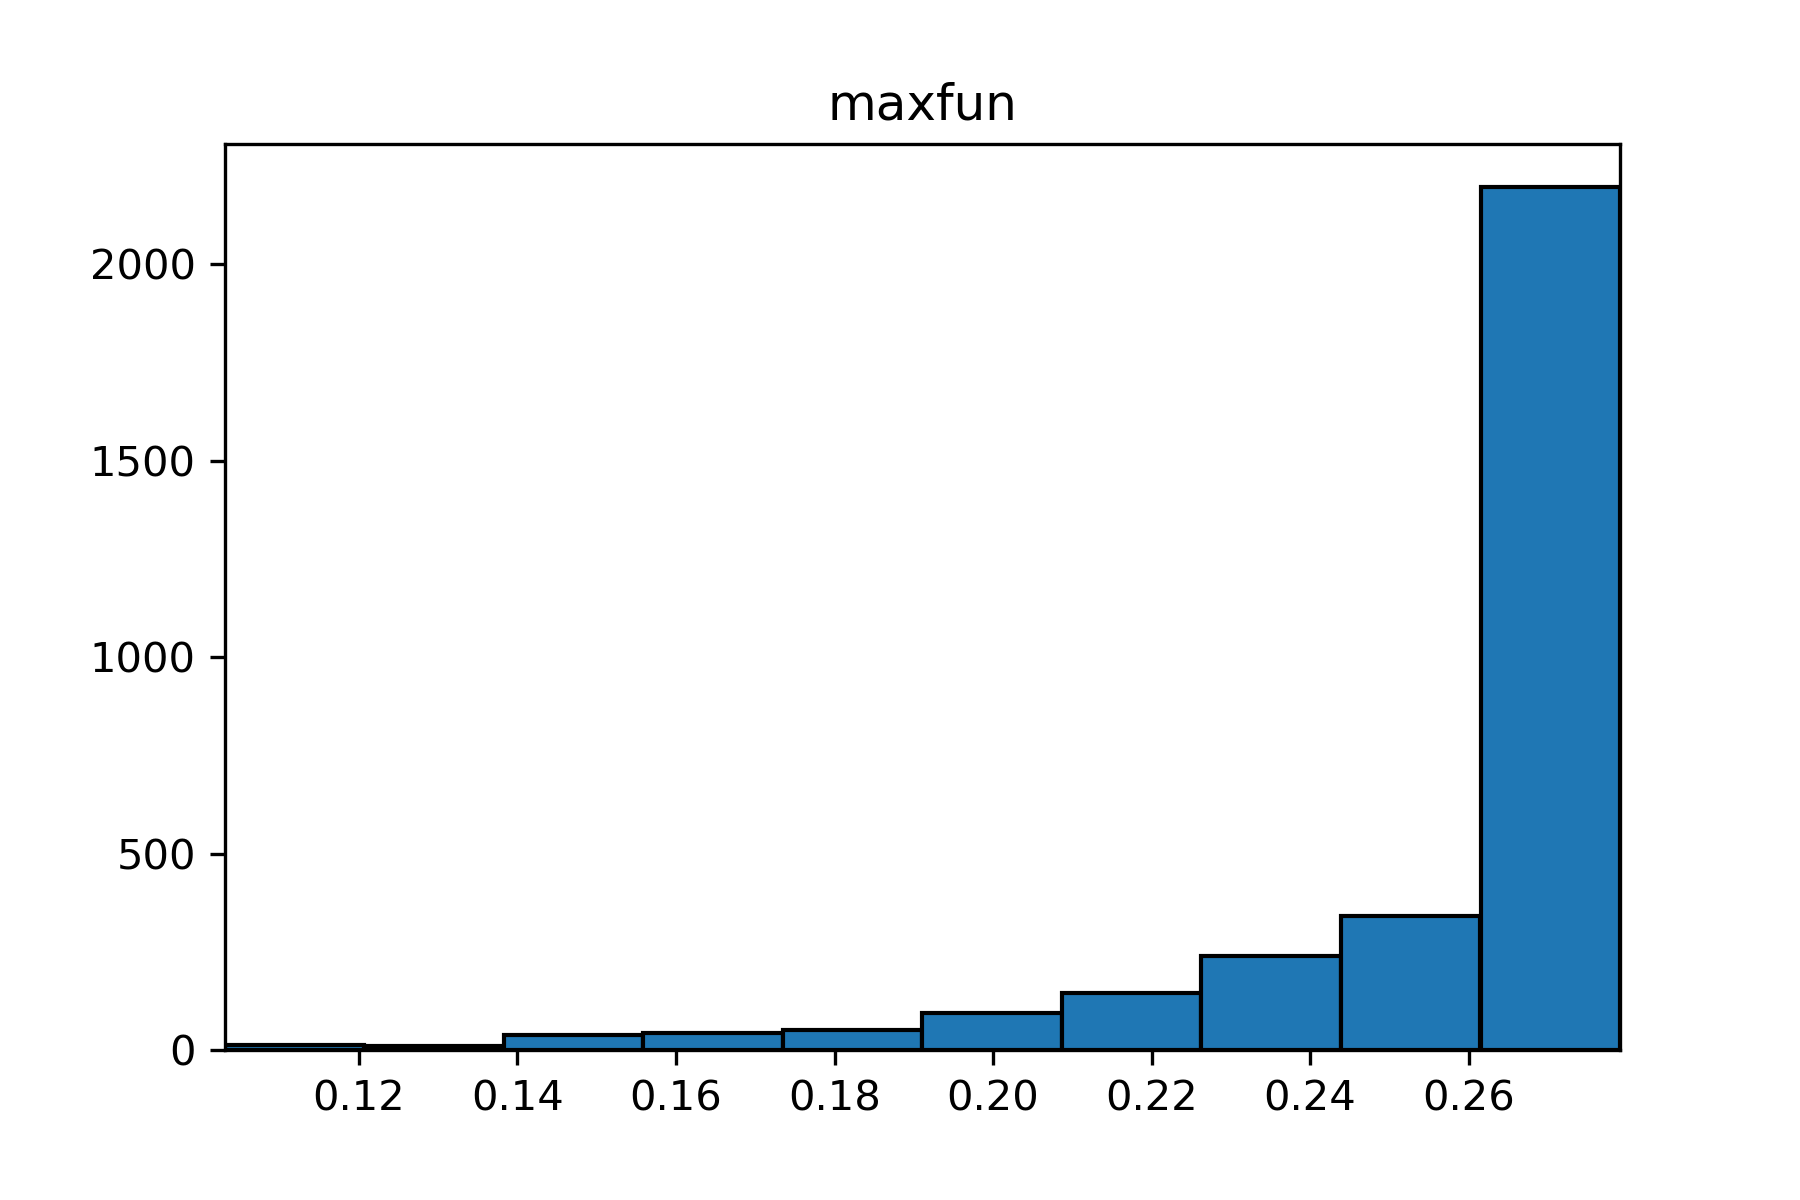
\includegraphics[width=3.85cm]{raw_13_maxfun}
        \caption{maxfun}
        \label{fig:sub_raw_14}
    \end{subfigure}\hfill
    % meandom
    \begin{subfigure}{0.32\textwidth}
        \centering
        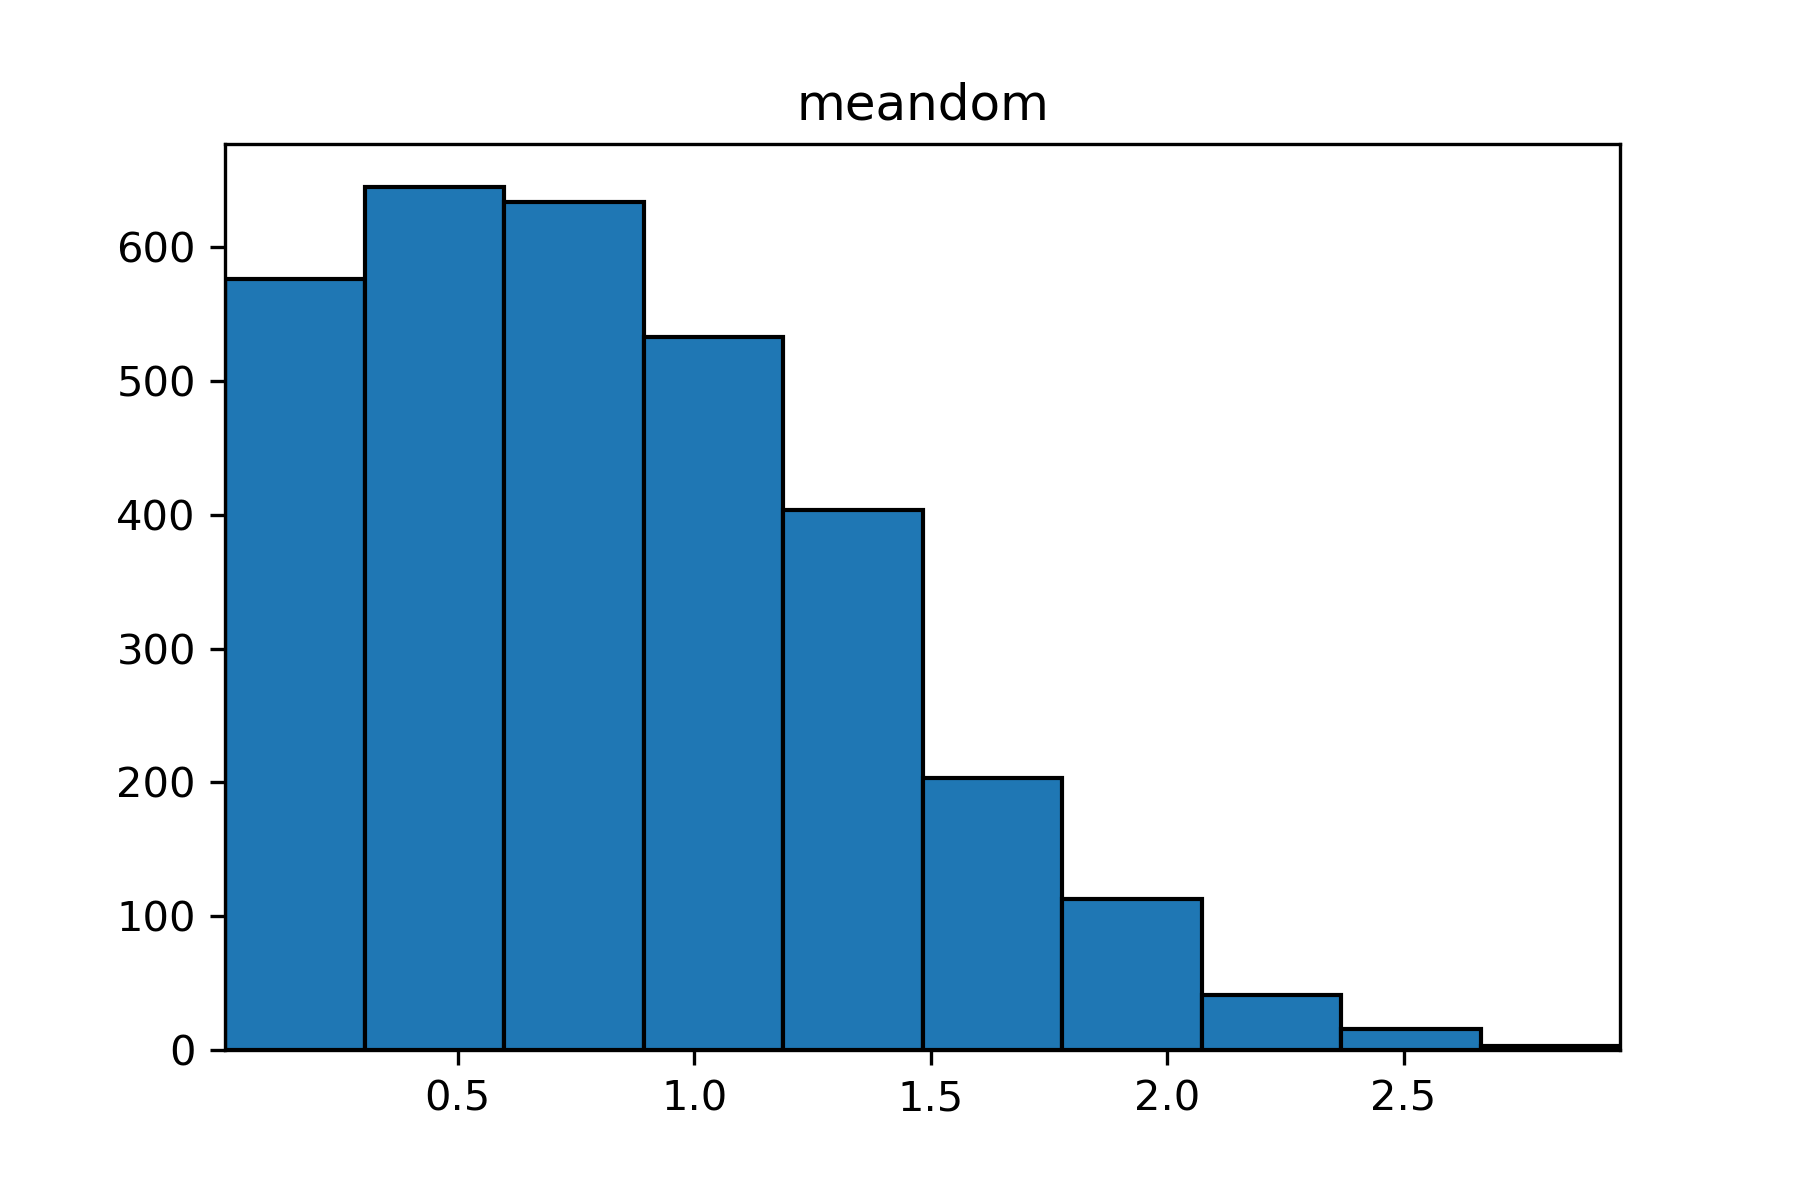
\includegraphics[width=3.85cm]{raw_14_meandom}
        \caption{meandom}
        \label{fig:sub_raw_15}
    \end{subfigure}\hfill
    % mindom
    \begin{subfigure}{0.32\textwidth}
        \centering
        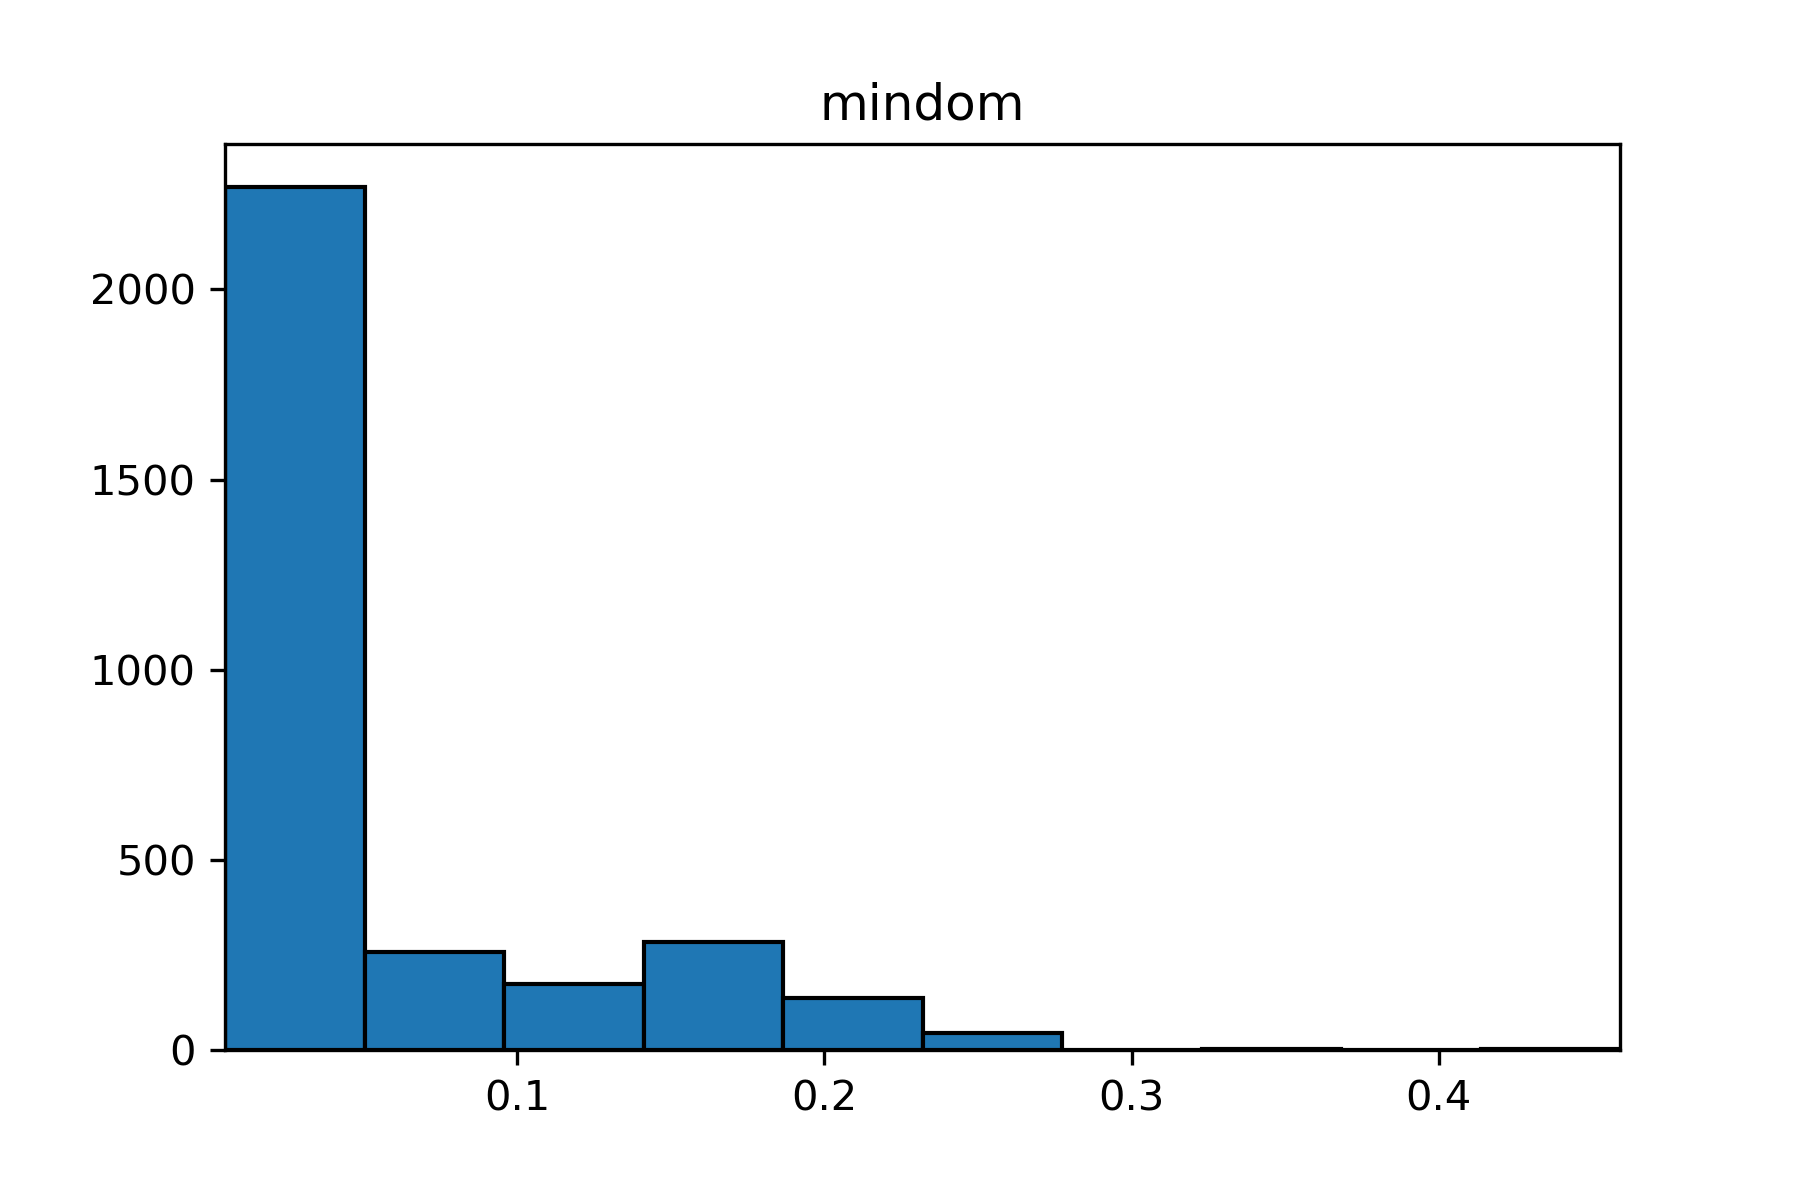
\includegraphics[width=3.85cm]{raw_15_mindom}
        \caption{mindom}
        \label{fig:sub_raw_16}
    \end{subfigure}\hfill
    % maxdom
    \begin{subfigure}{0.32\textwidth}
        \centering
        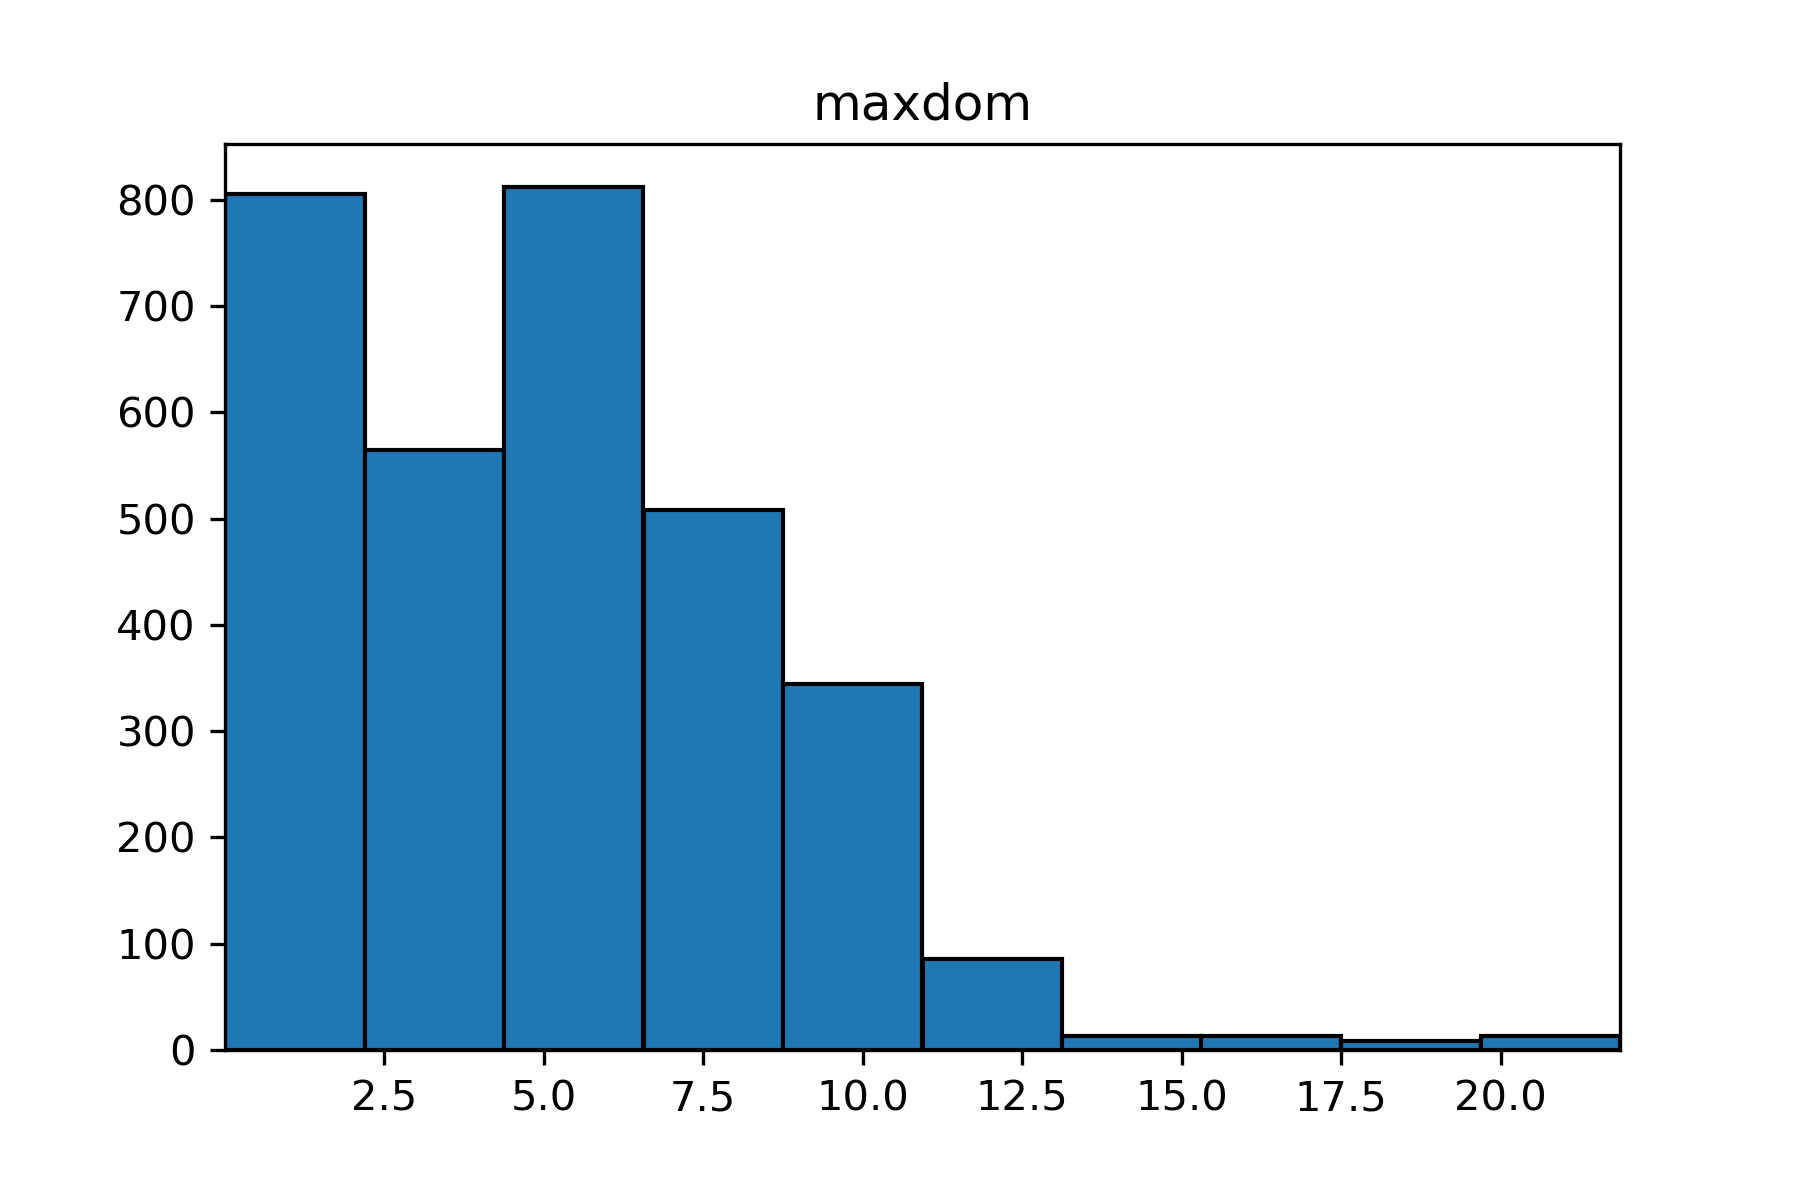
\includegraphics[width=3.85cm]{raw_16_maxdom}
        \caption{maxdom}
        \label{fig:sub_raw_17}
    \end{subfigure}\hfill
    % dfrange
    \begin{subfigure}{0.32\textwidth}
        \centering
        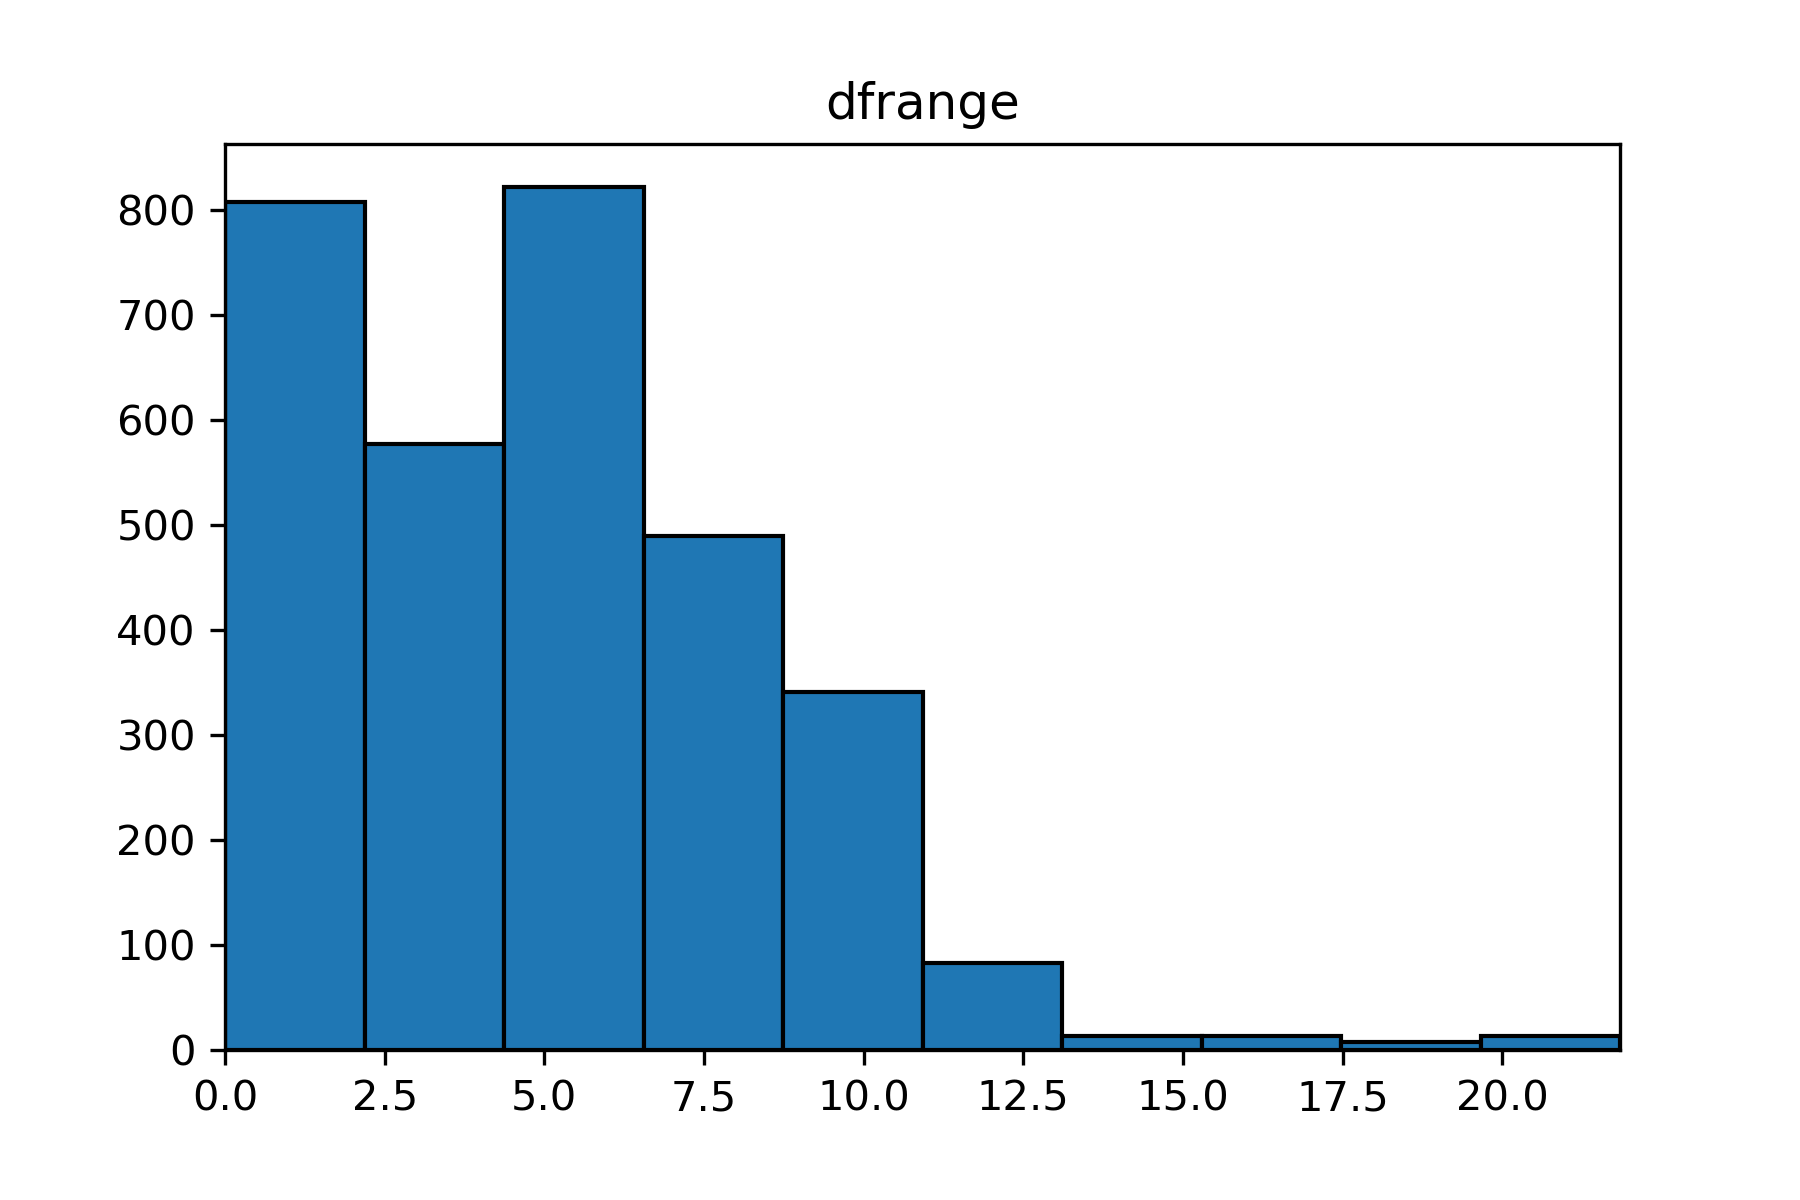
\includegraphics[width=3.85cm]{raw_17_dfrange}
        \caption{dfrange}
        \label{fig:sub_raw_18}
    \end{subfigure}\hfill
    % modindx
    \begin{subfigure}{0.32\textwidth}
        \centering
        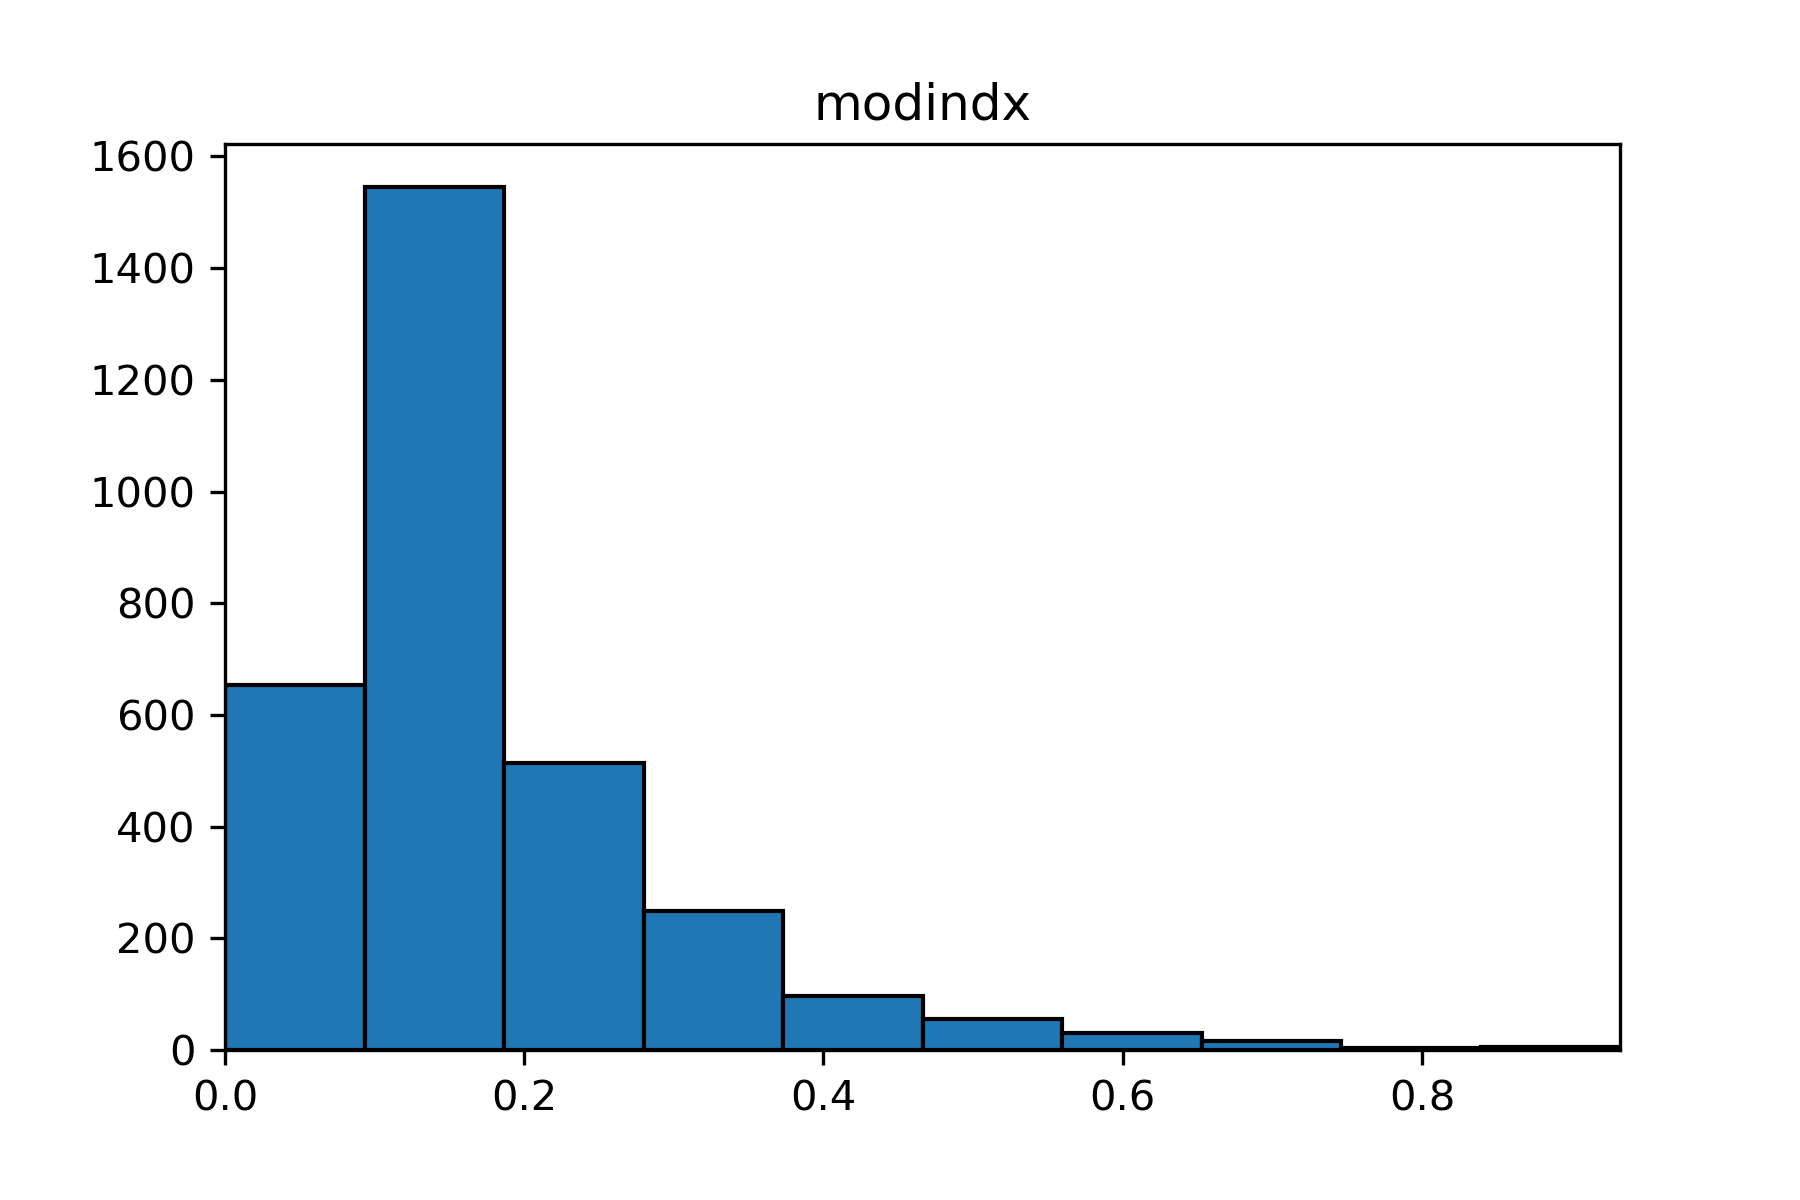
\includegraphics[width=3.85cm]{raw_18_modindx}
        \caption{modindx}
        \label{fig:sub_raw_19}
    \end{subfigure}
    % caption and label
    \caption{Histograms of raw input features}
    \label{fig:pre-ex1-raw_histograms}
\end{figure}

% histograms of stardardized features

\begin{figure}[H]
    \centering
    % sd
    \begin{subfigure}{0.32\textwidth}
        \centering
        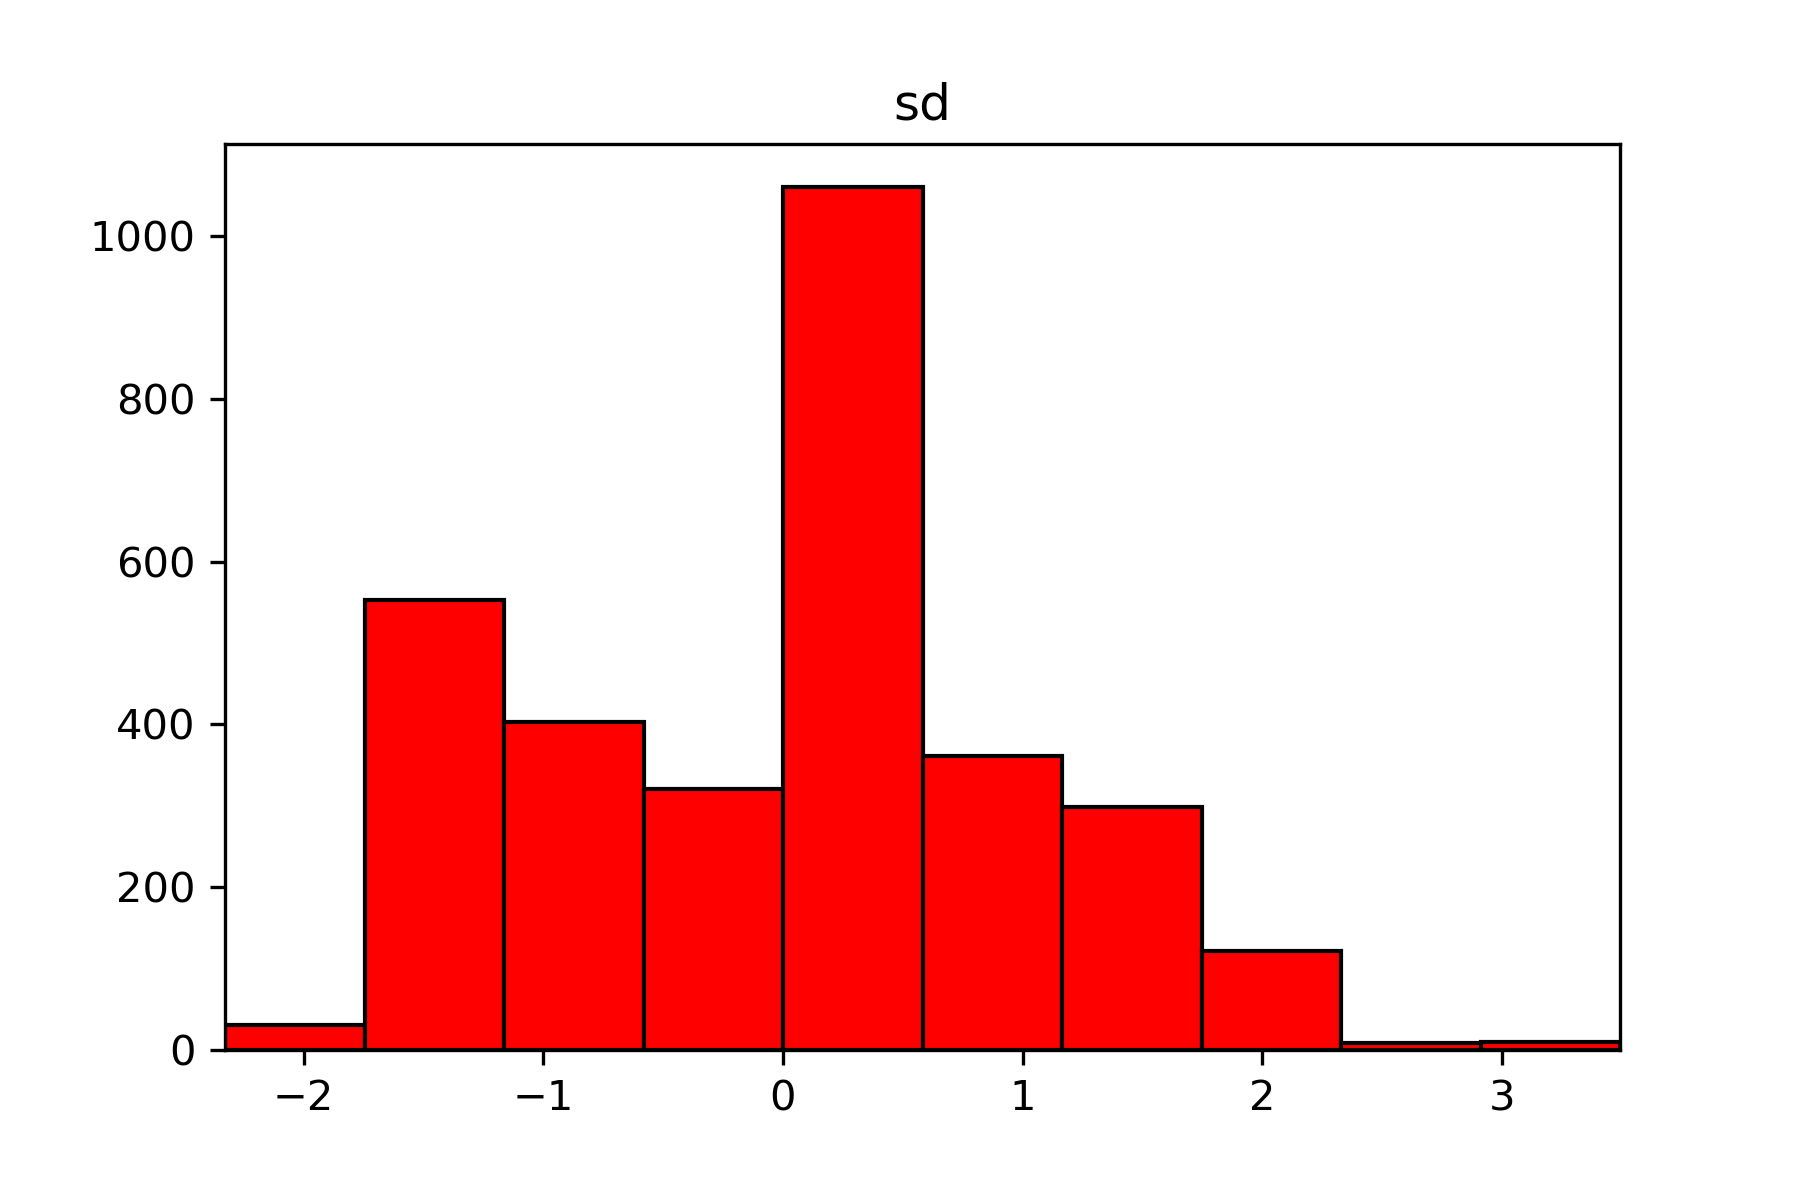
\includegraphics[width=3.85cm]{std_0_sd}
        \caption{sd}
        \label{fig:sub_std_1}
    \end{subfigure}
    \hfill
    % median
    \begin{subfigure}{0.32\textwidth}
        \centering
        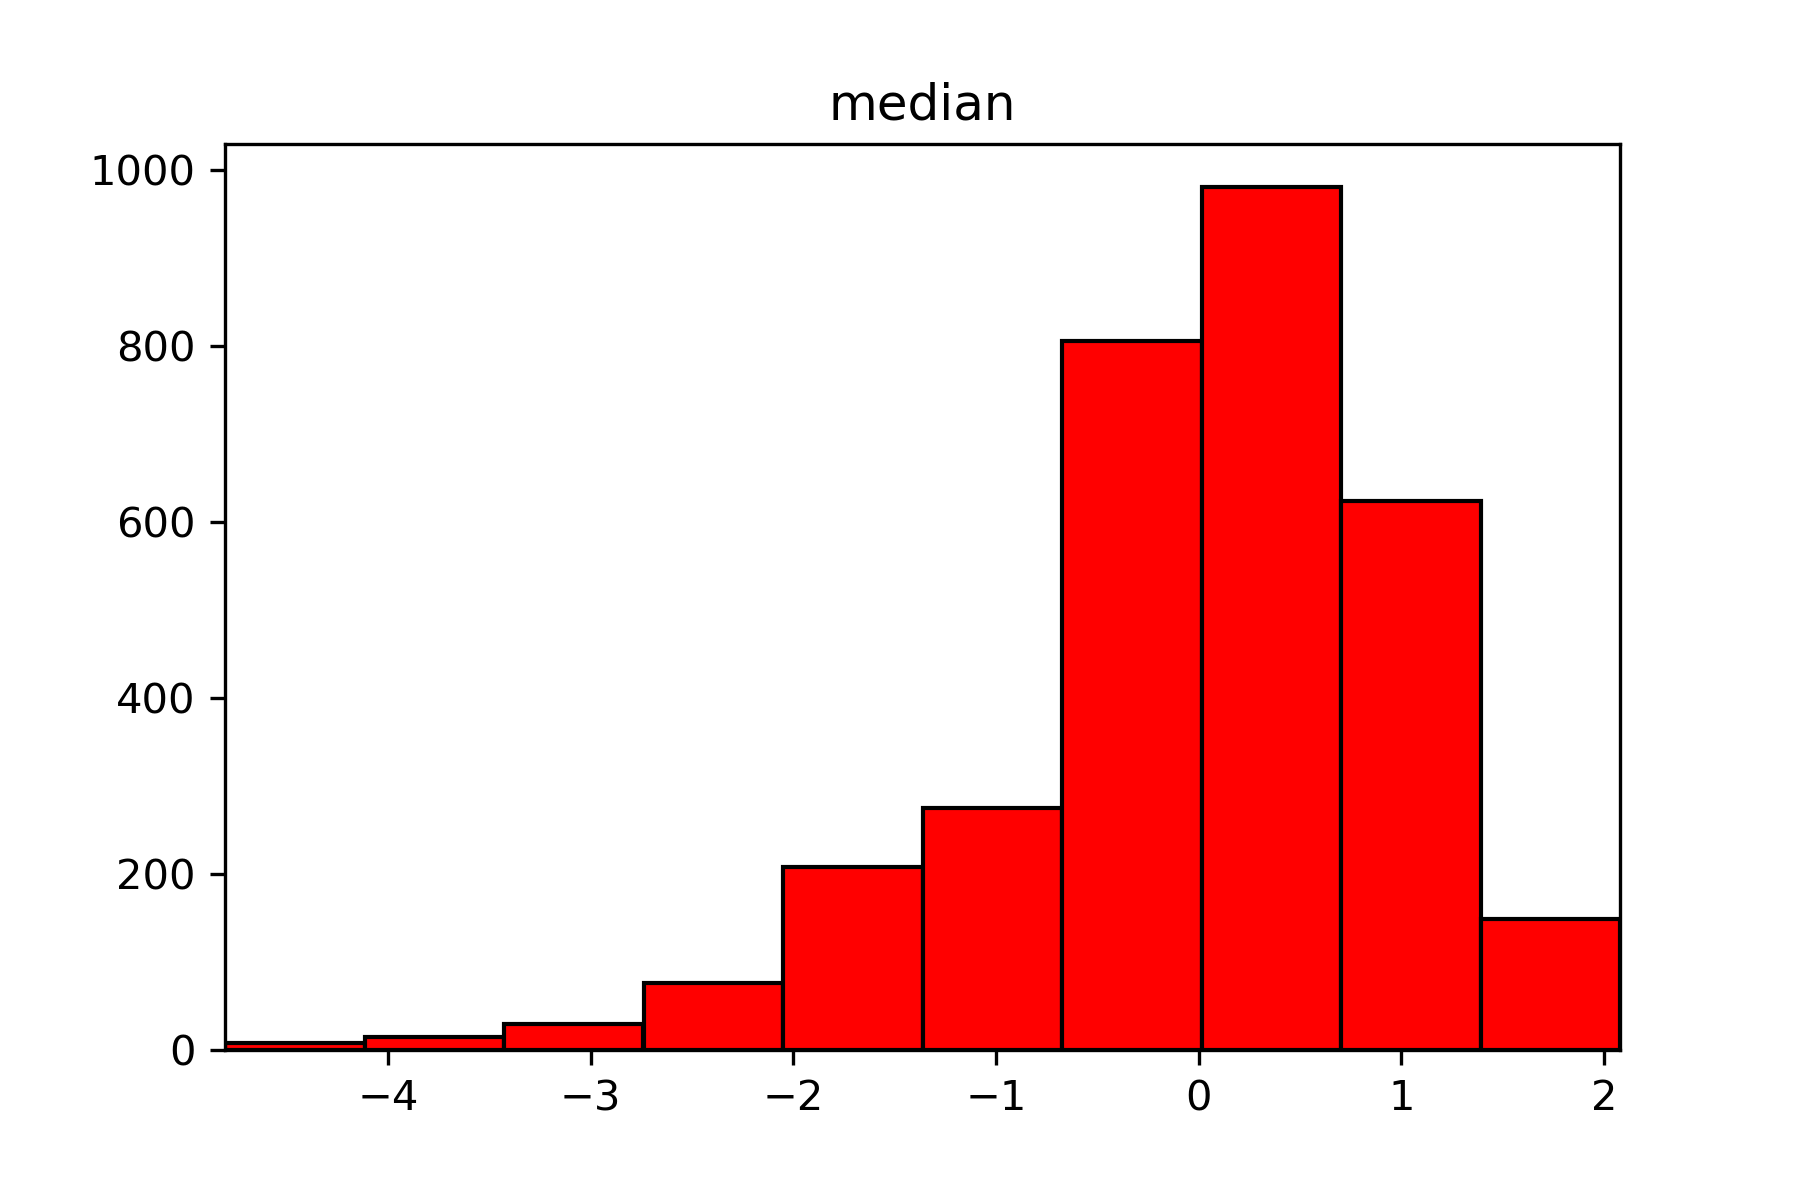
\includegraphics[width=3.85cm]{std_1_median}
        \caption{median}
        \label{fig:sub_std_2}
    \end{subfigure}
    \hfill
    % Q25
    \begin{subfigure}{0.32\textwidth}
        \centering
        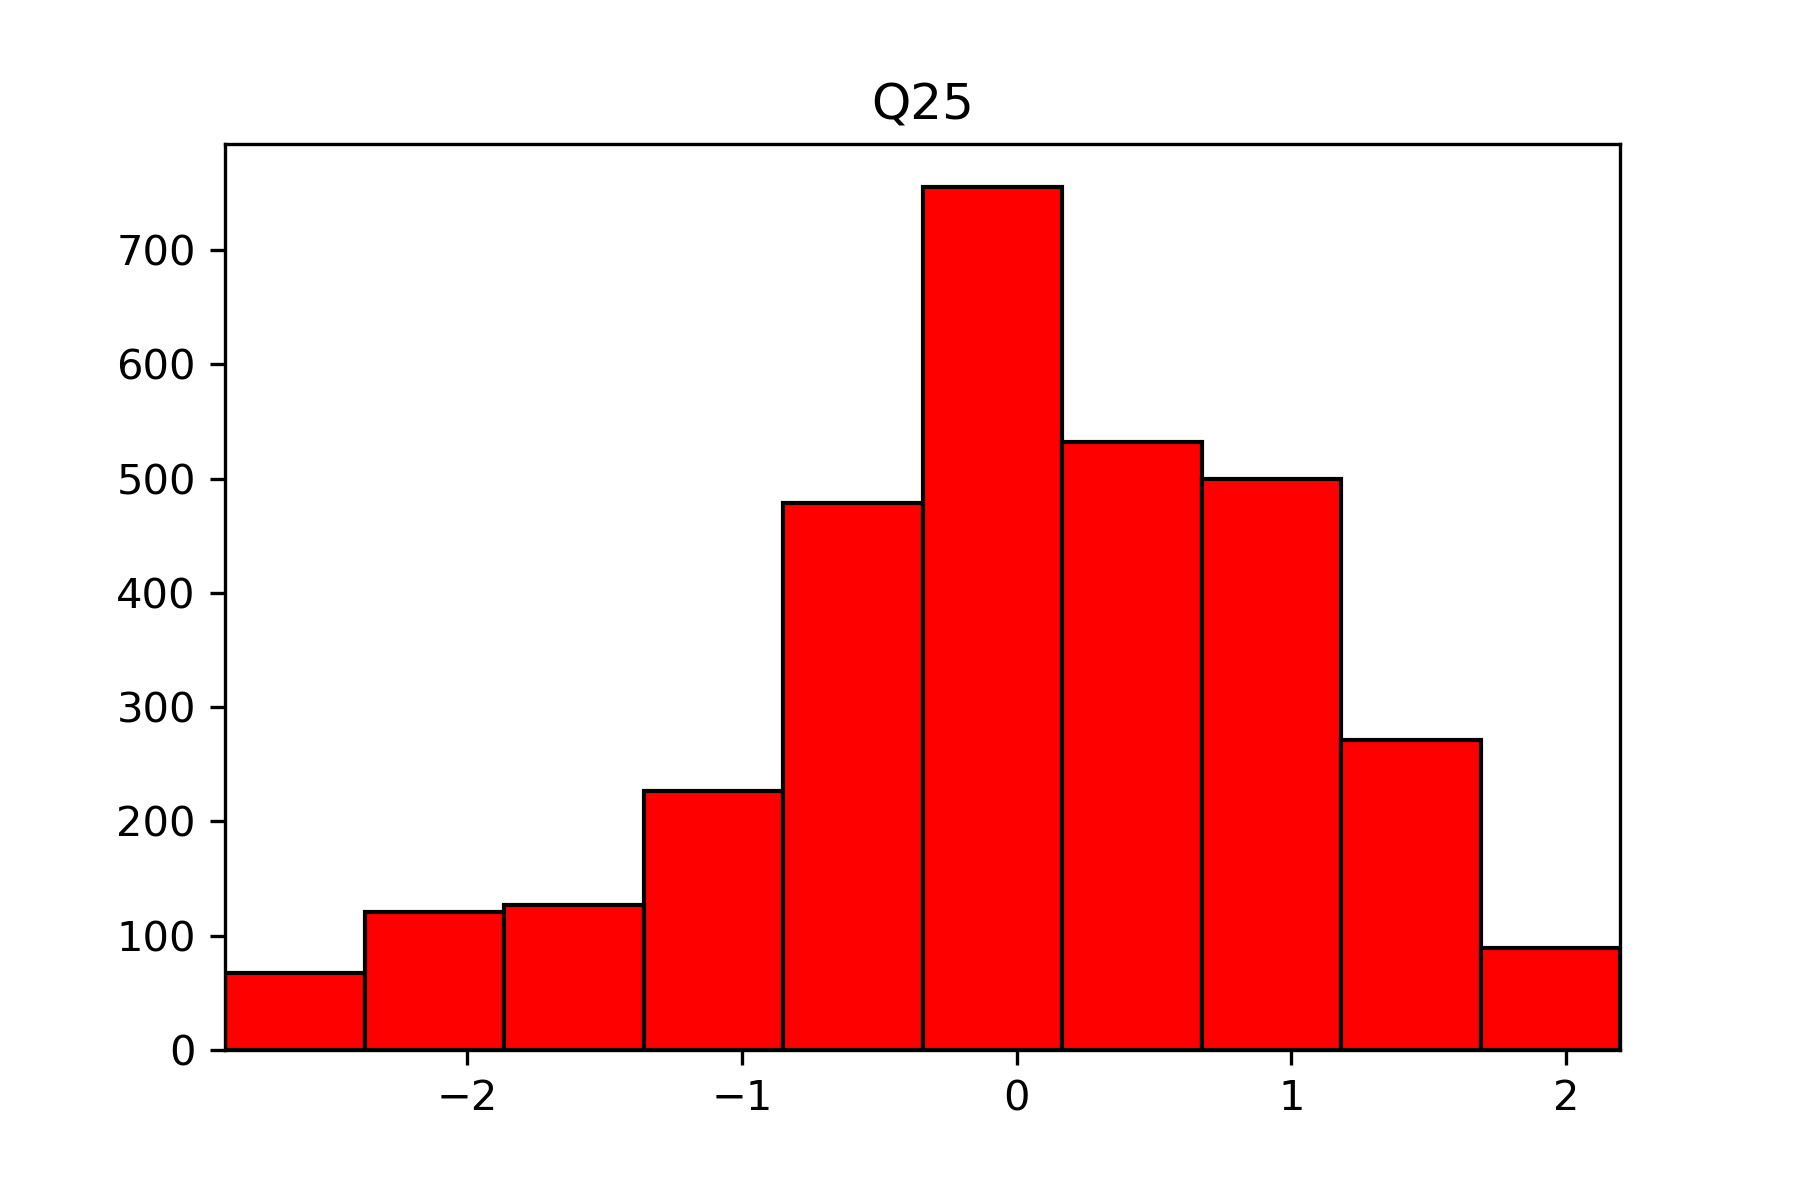
\includegraphics[width=3.85cm]{std_2_Q25}
        \caption{Q25}
        \label{fig:sub_std_3}
    \end{subfigure}%
    \\
    % Q75
    \begin{subfigure}{0.32\textwidth}
        \centering
        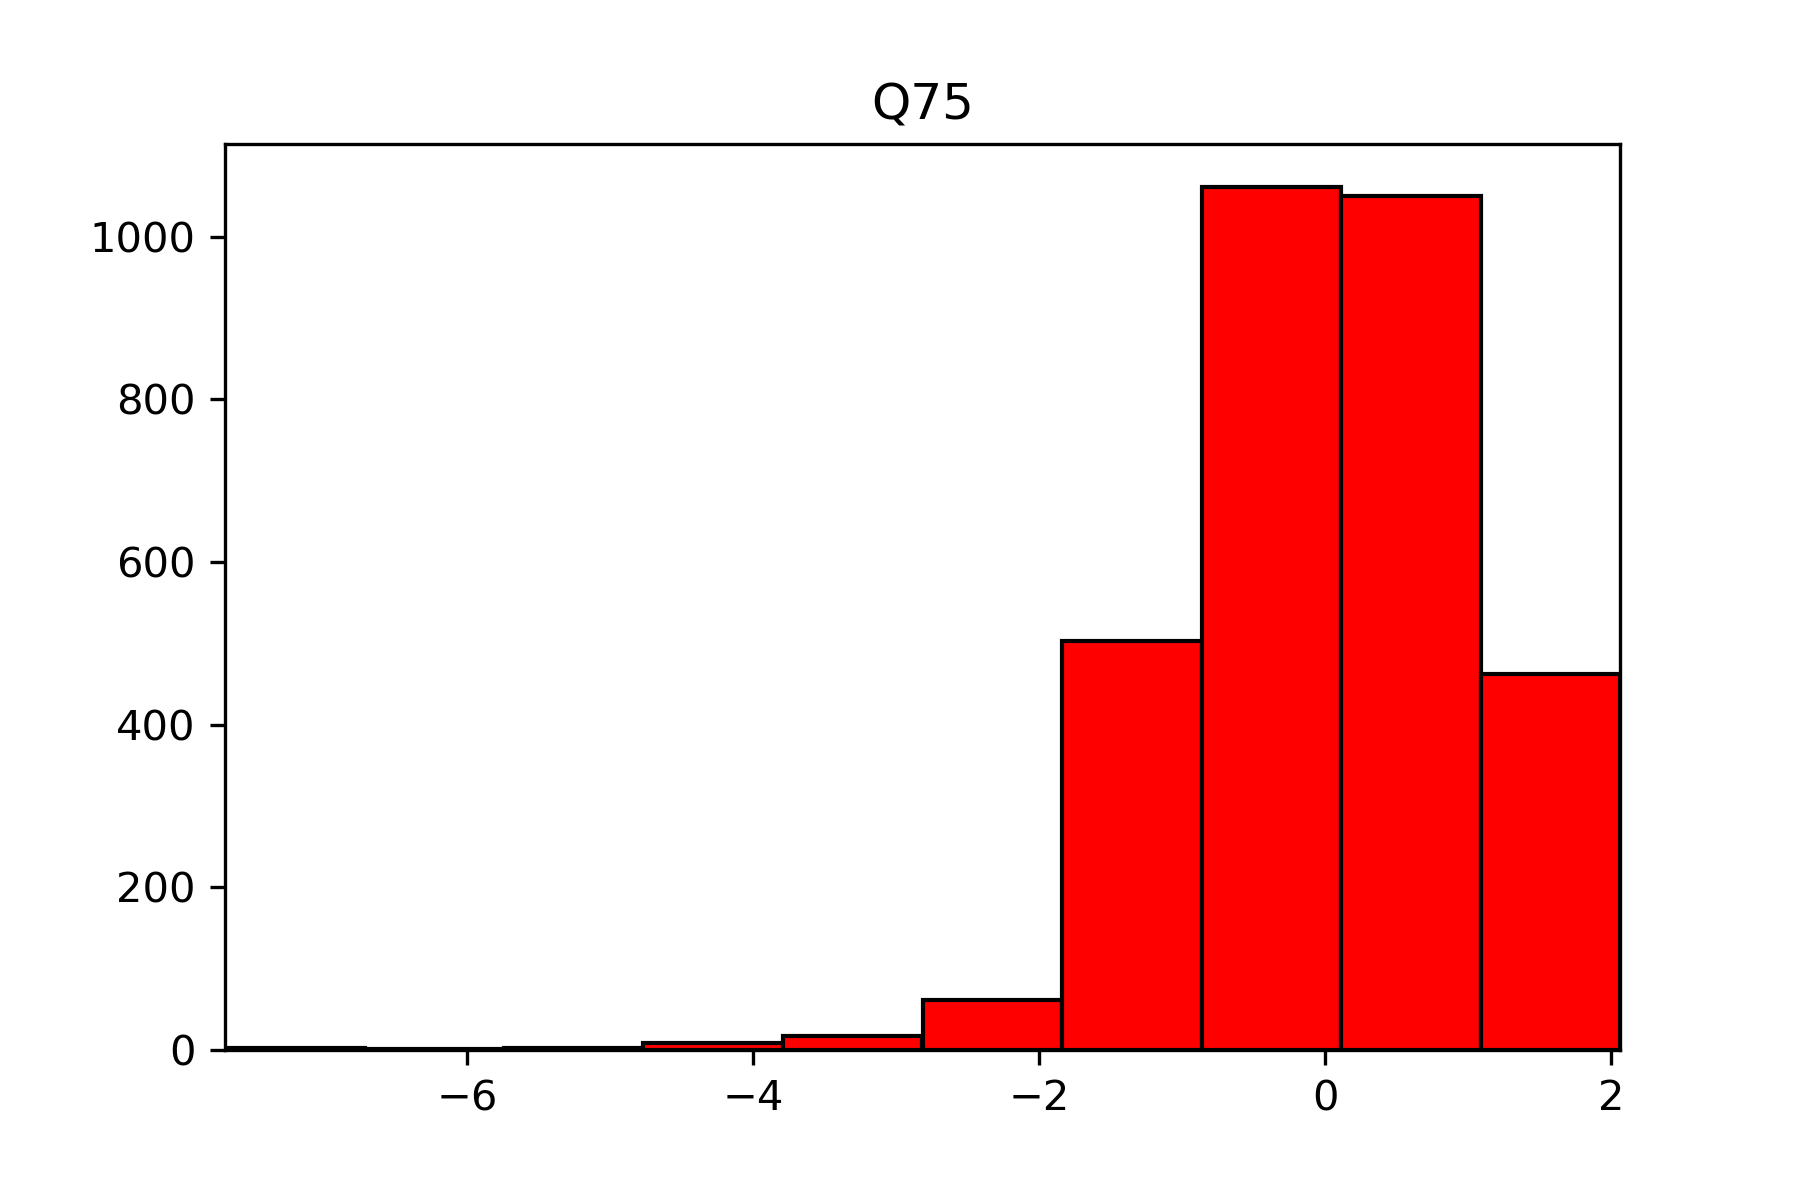
\includegraphics[width=3.85cm]{std_3_Q75}
        \caption{Q75}
        \label{fig:sub_std_4}
    \end{subfigure}\hfill
    % Q75
    \begin{subfigure}{0.32\textwidth}
        \centering
        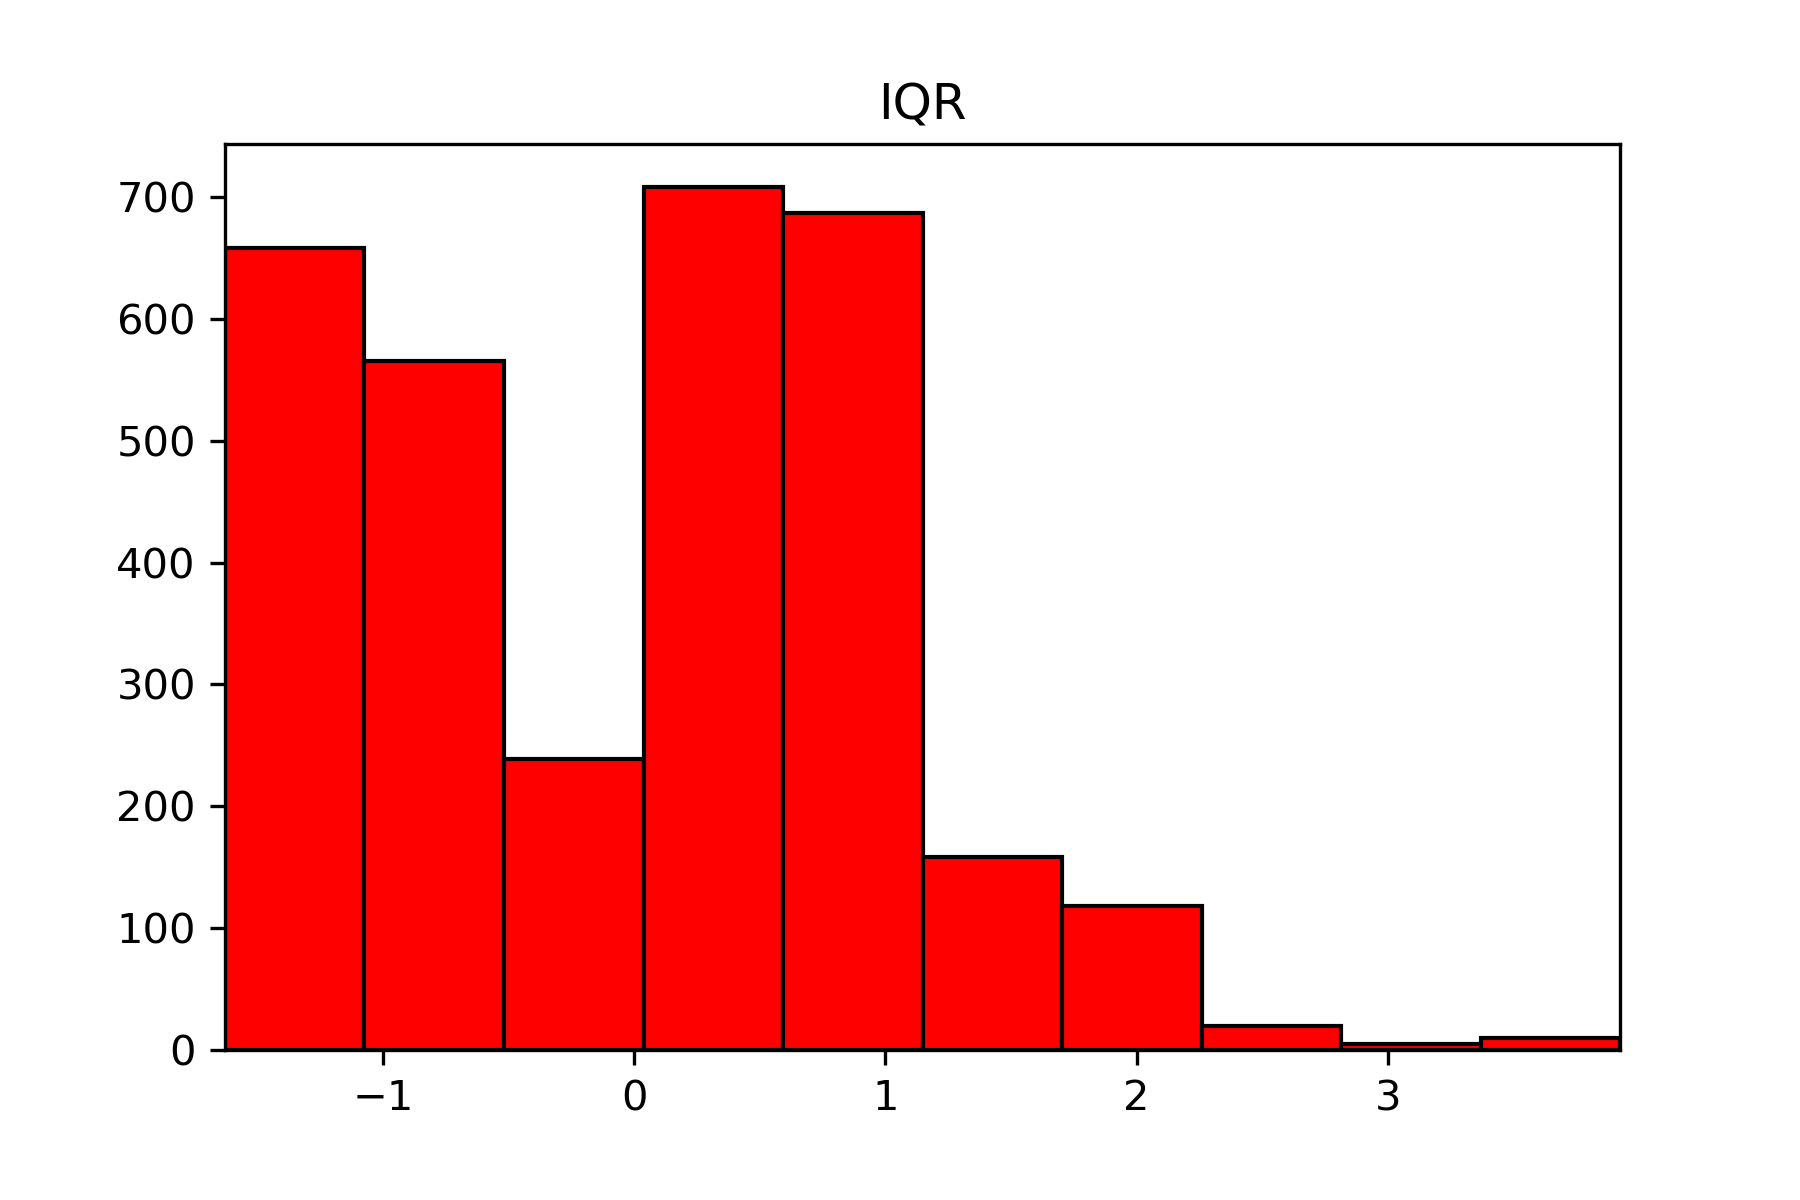
\includegraphics[width=3.85cm]{std_4_IQR}
        \caption{IQR}
        \label{fig:sub_std_5}
    \end{subfigure}\hfill
    % skew
    \begin{subfigure}{0.32\textwidth}
        \centering
        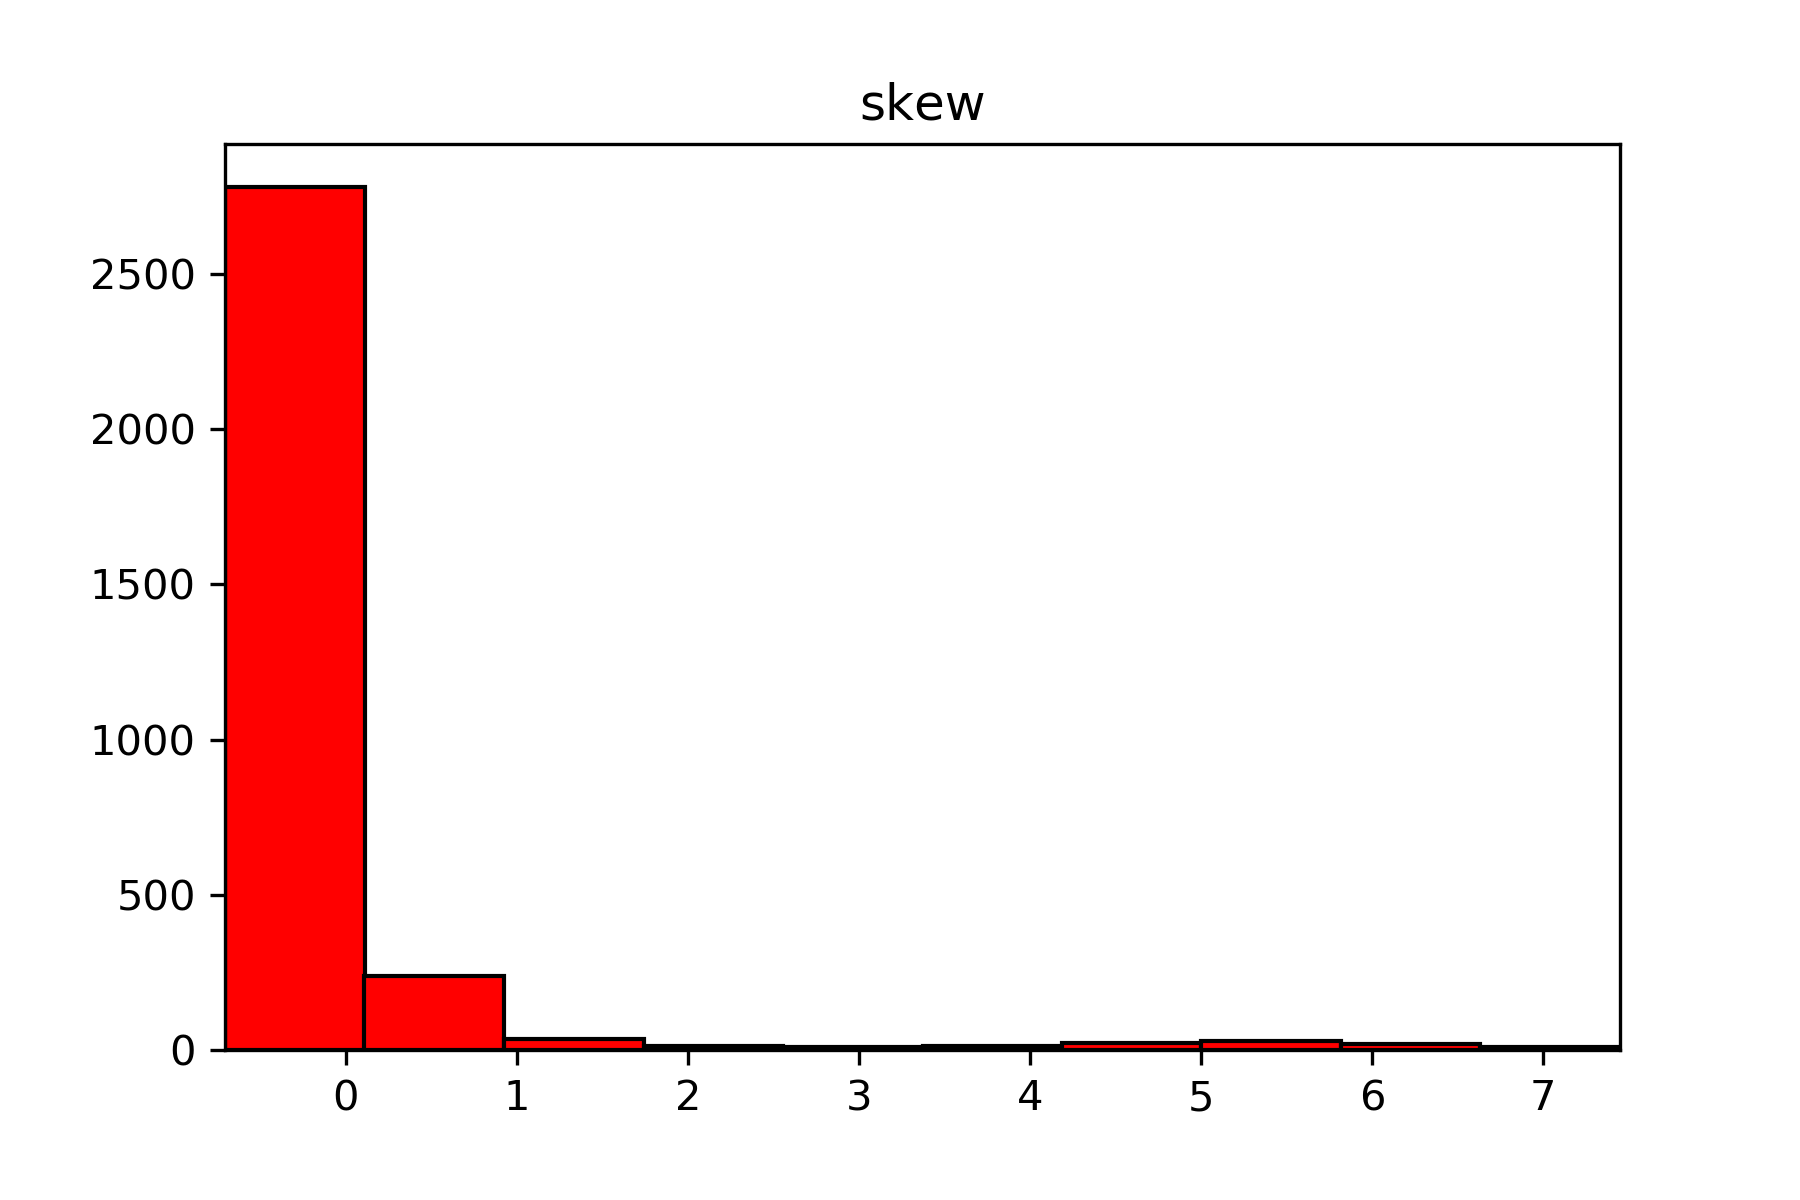
\includegraphics[width=3.85cm]{std_5_skew}
        \caption{skew}
        \label{fig:sub_std_6}
    \end{subfigure}
    \\
    % kurt
    \begin{subfigure}{0.32\textwidth}
        \centering
        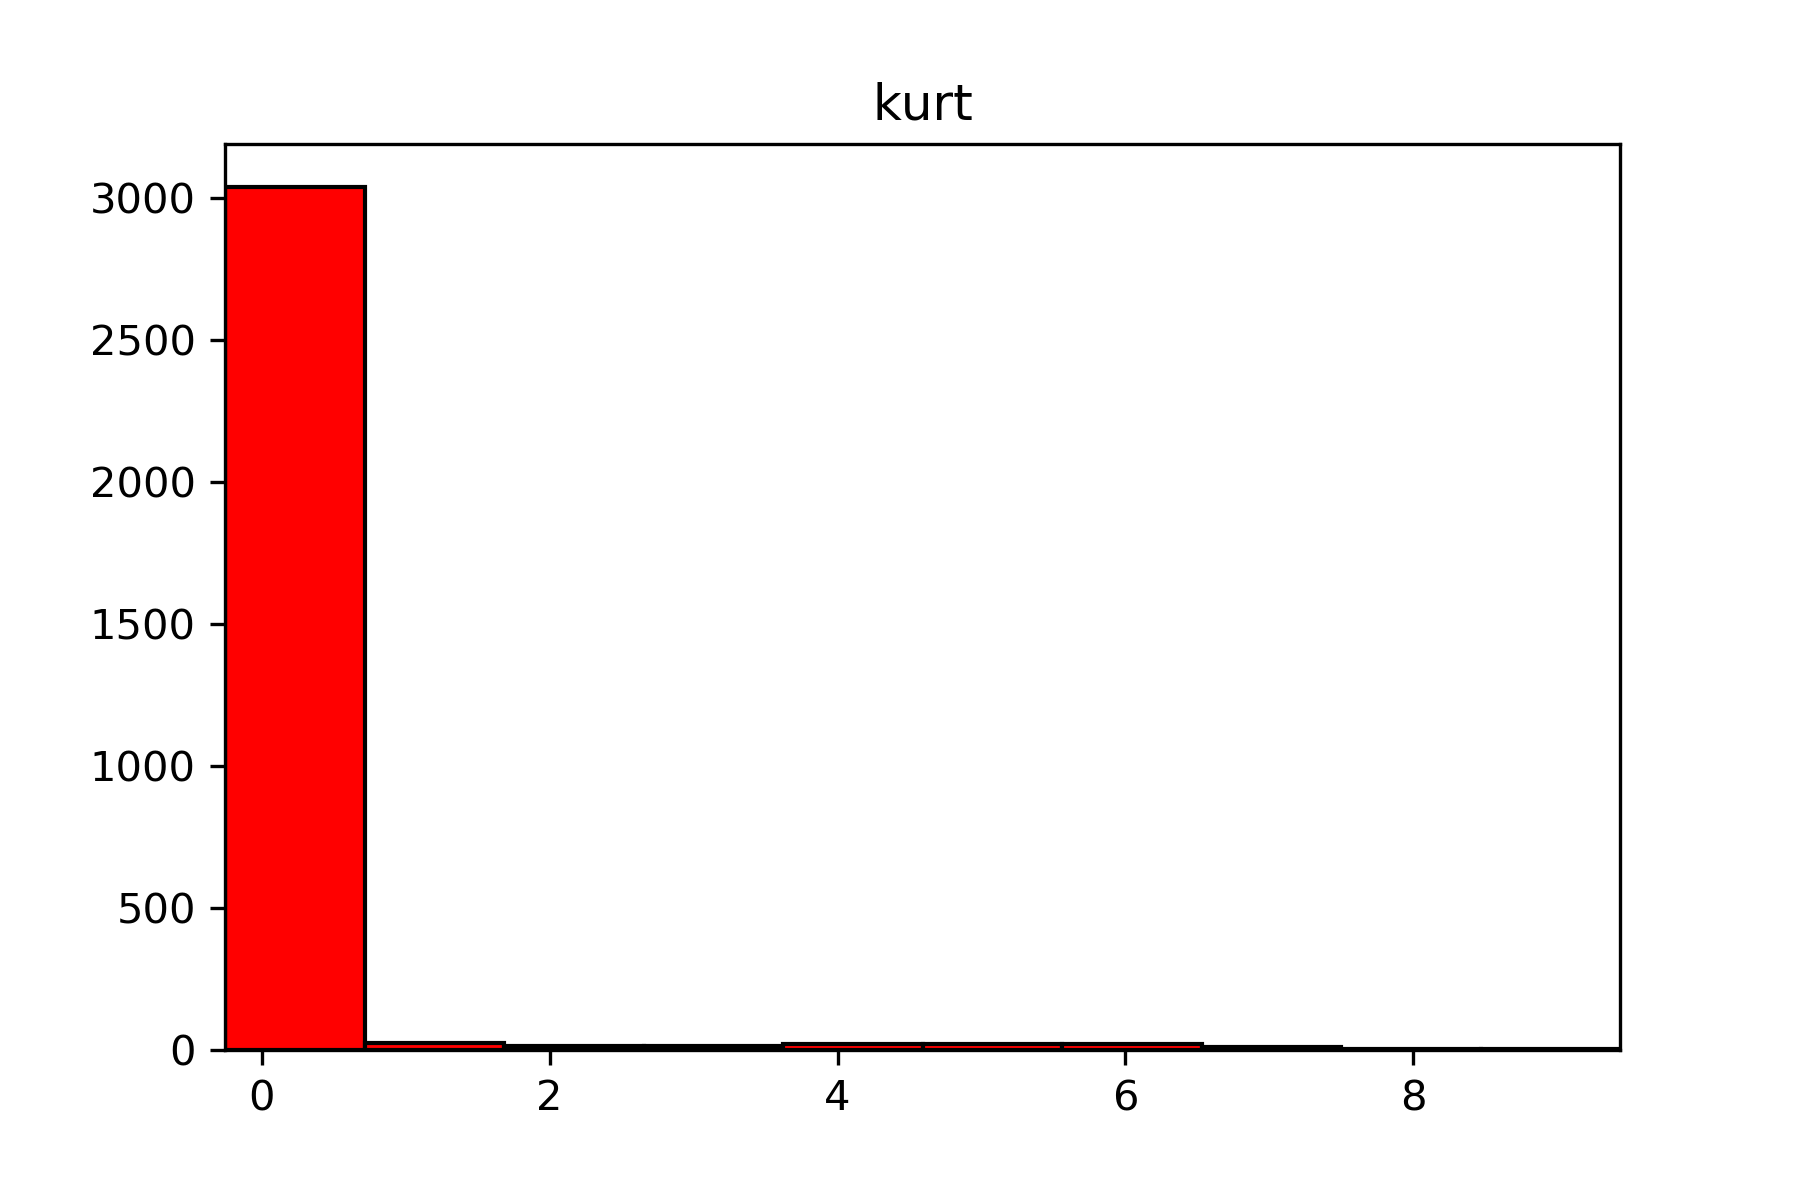
\includegraphics[width=3.85cm]{std_6_kurt}
        \caption{kurt}
        \label{fig:sub_std_7}
    \end{subfigure}\hfill
    % sp ent
    \begin{subfigure}{0.32\textwidth}
        \centering
        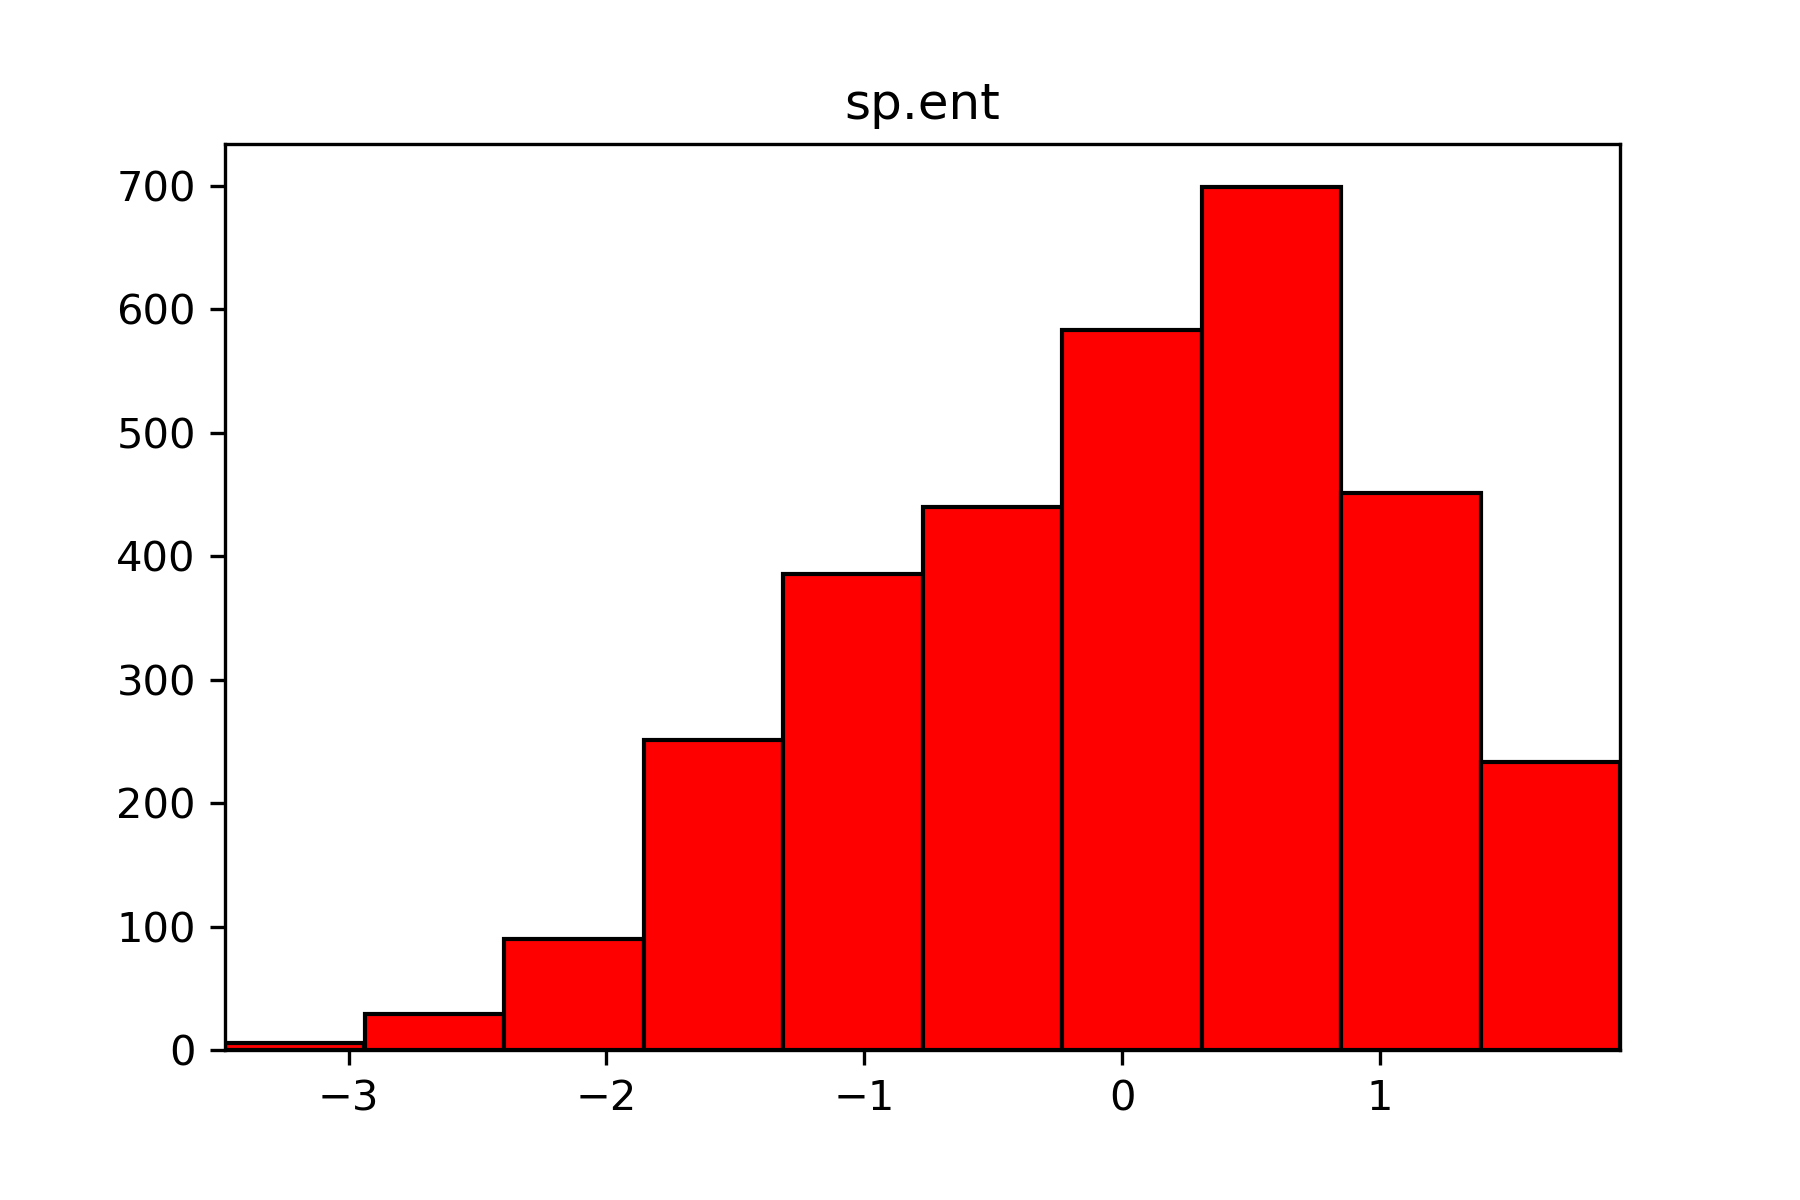
\includegraphics[width=3.85cm]{std_7_sp_ent}
        \caption{sp ent}
        \label{fig:sub_std_8}
    \end{subfigure}\hfill
    % sfm
    \begin{subfigure}{0.32\textwidth}
        \centering
        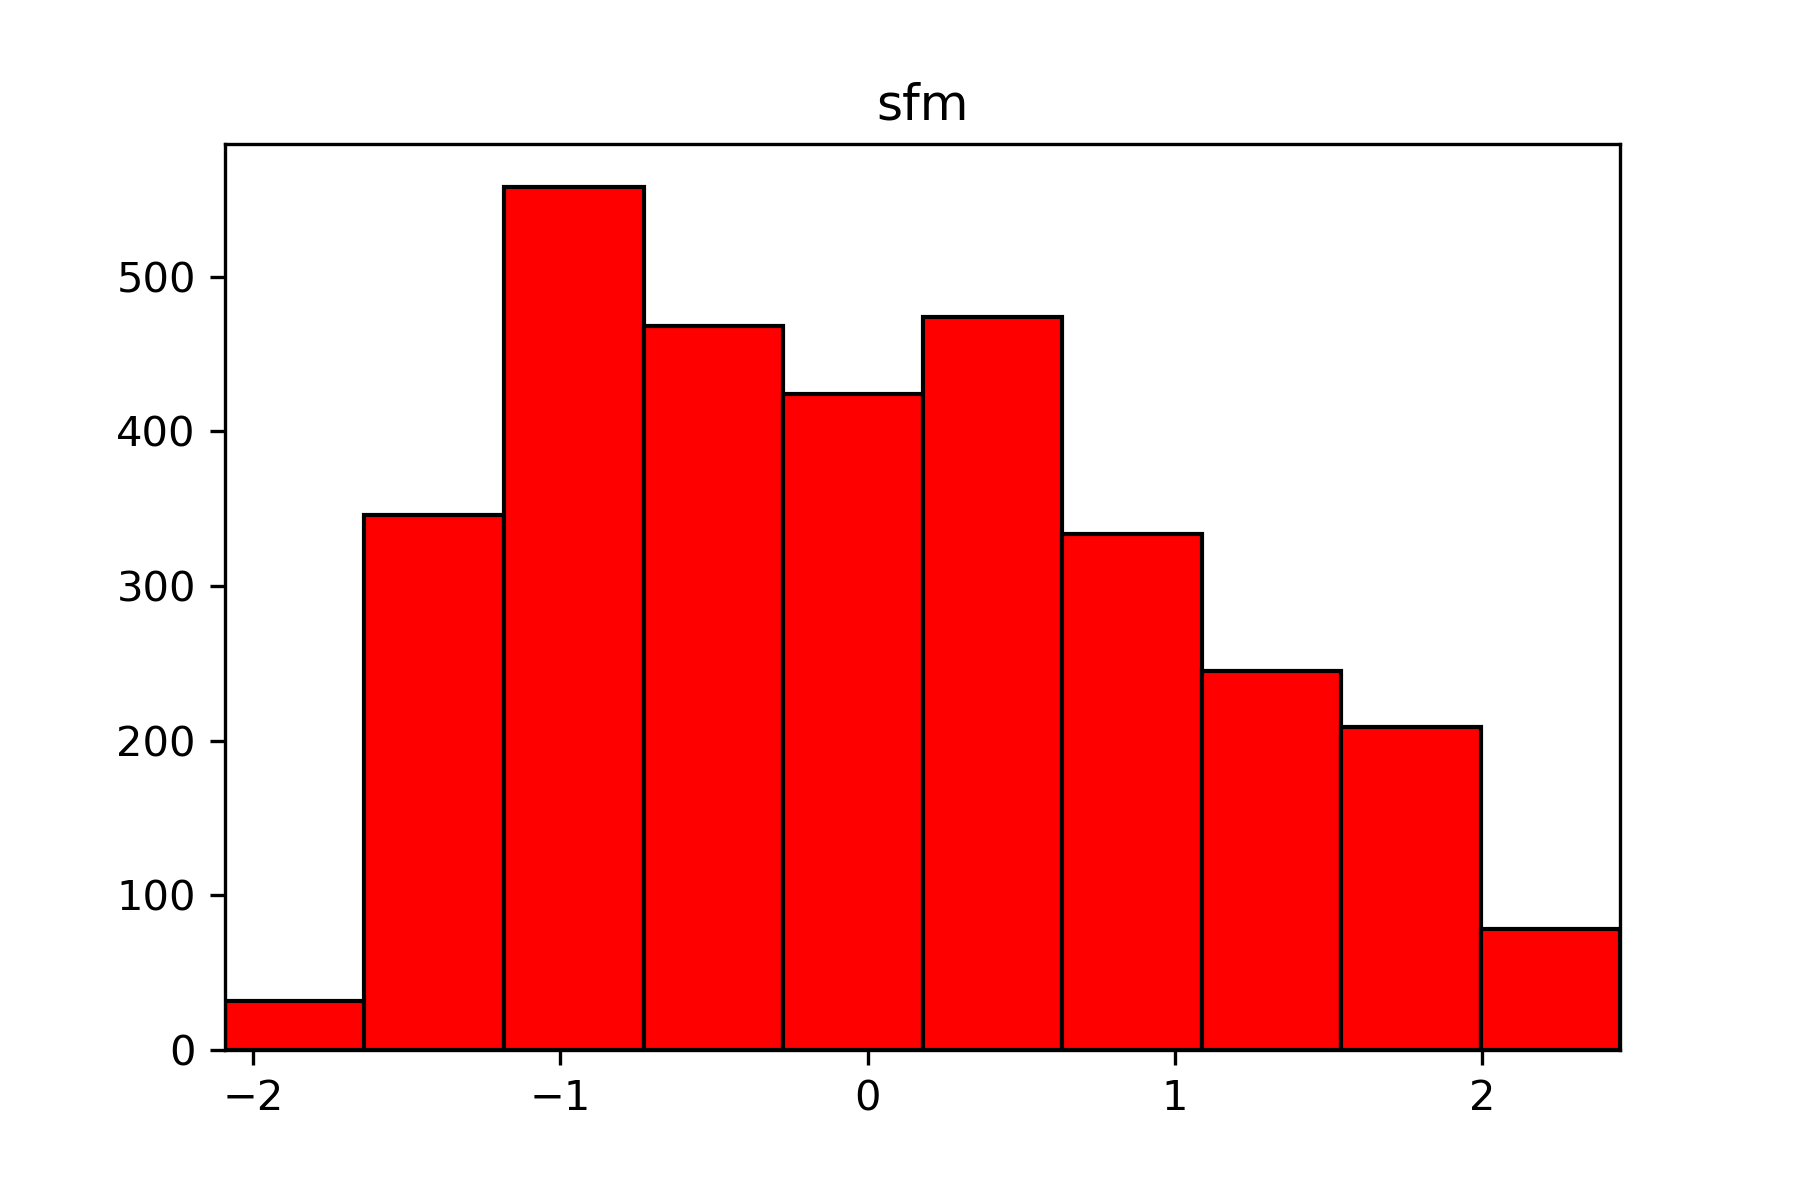
\includegraphics[width=3.85cm]{std_8_sfm}
        \caption{smf}
        \label{fig:sub_std_9}
    \end{subfigure}\hfill
    % mode
    \begin{subfigure}{0.32\textwidth}
        \centering
        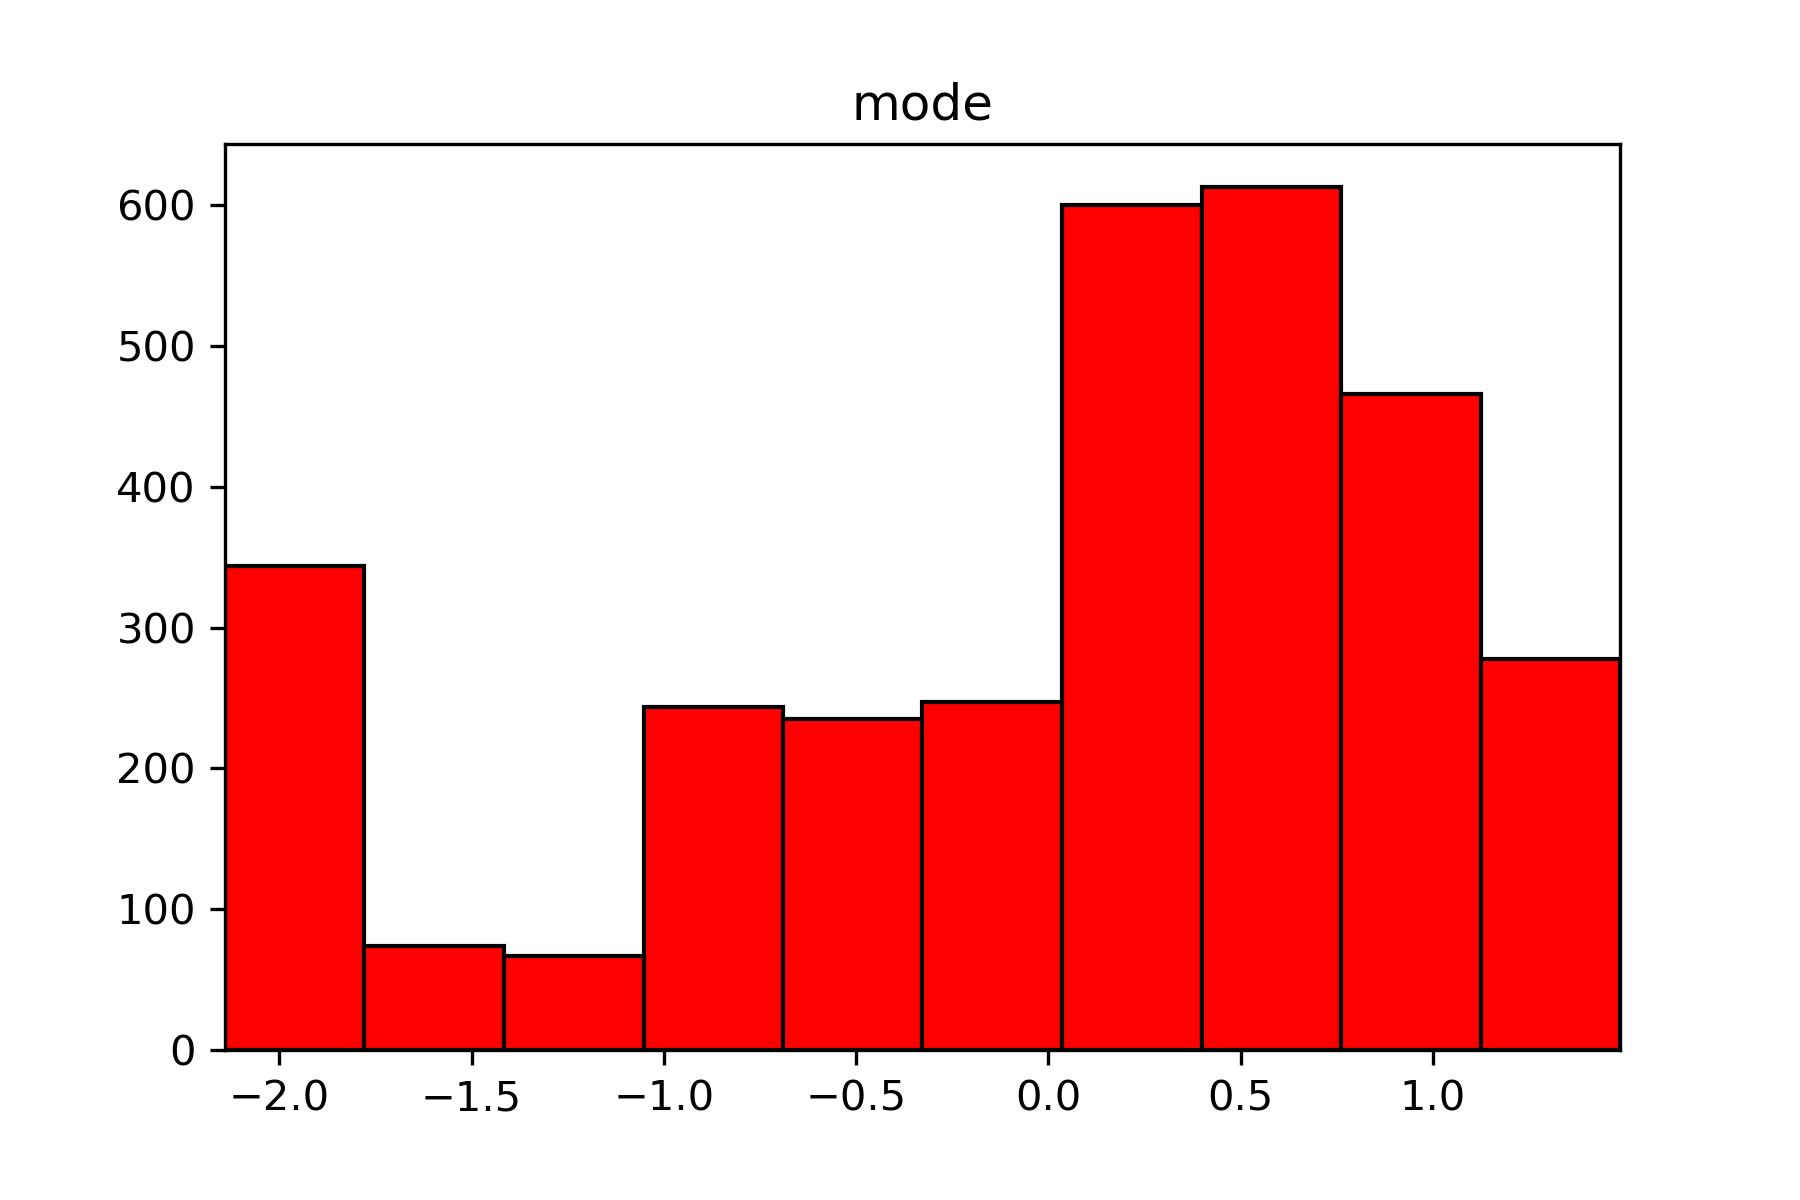
\includegraphics[width=3.85cm]{std_9_mode}
        \caption{mode}
        \label{fig:sub_std_10}
    \end{subfigure}\hfill
    % centroid
    \begin{subfigure}{0.32\textwidth}
        \centering
        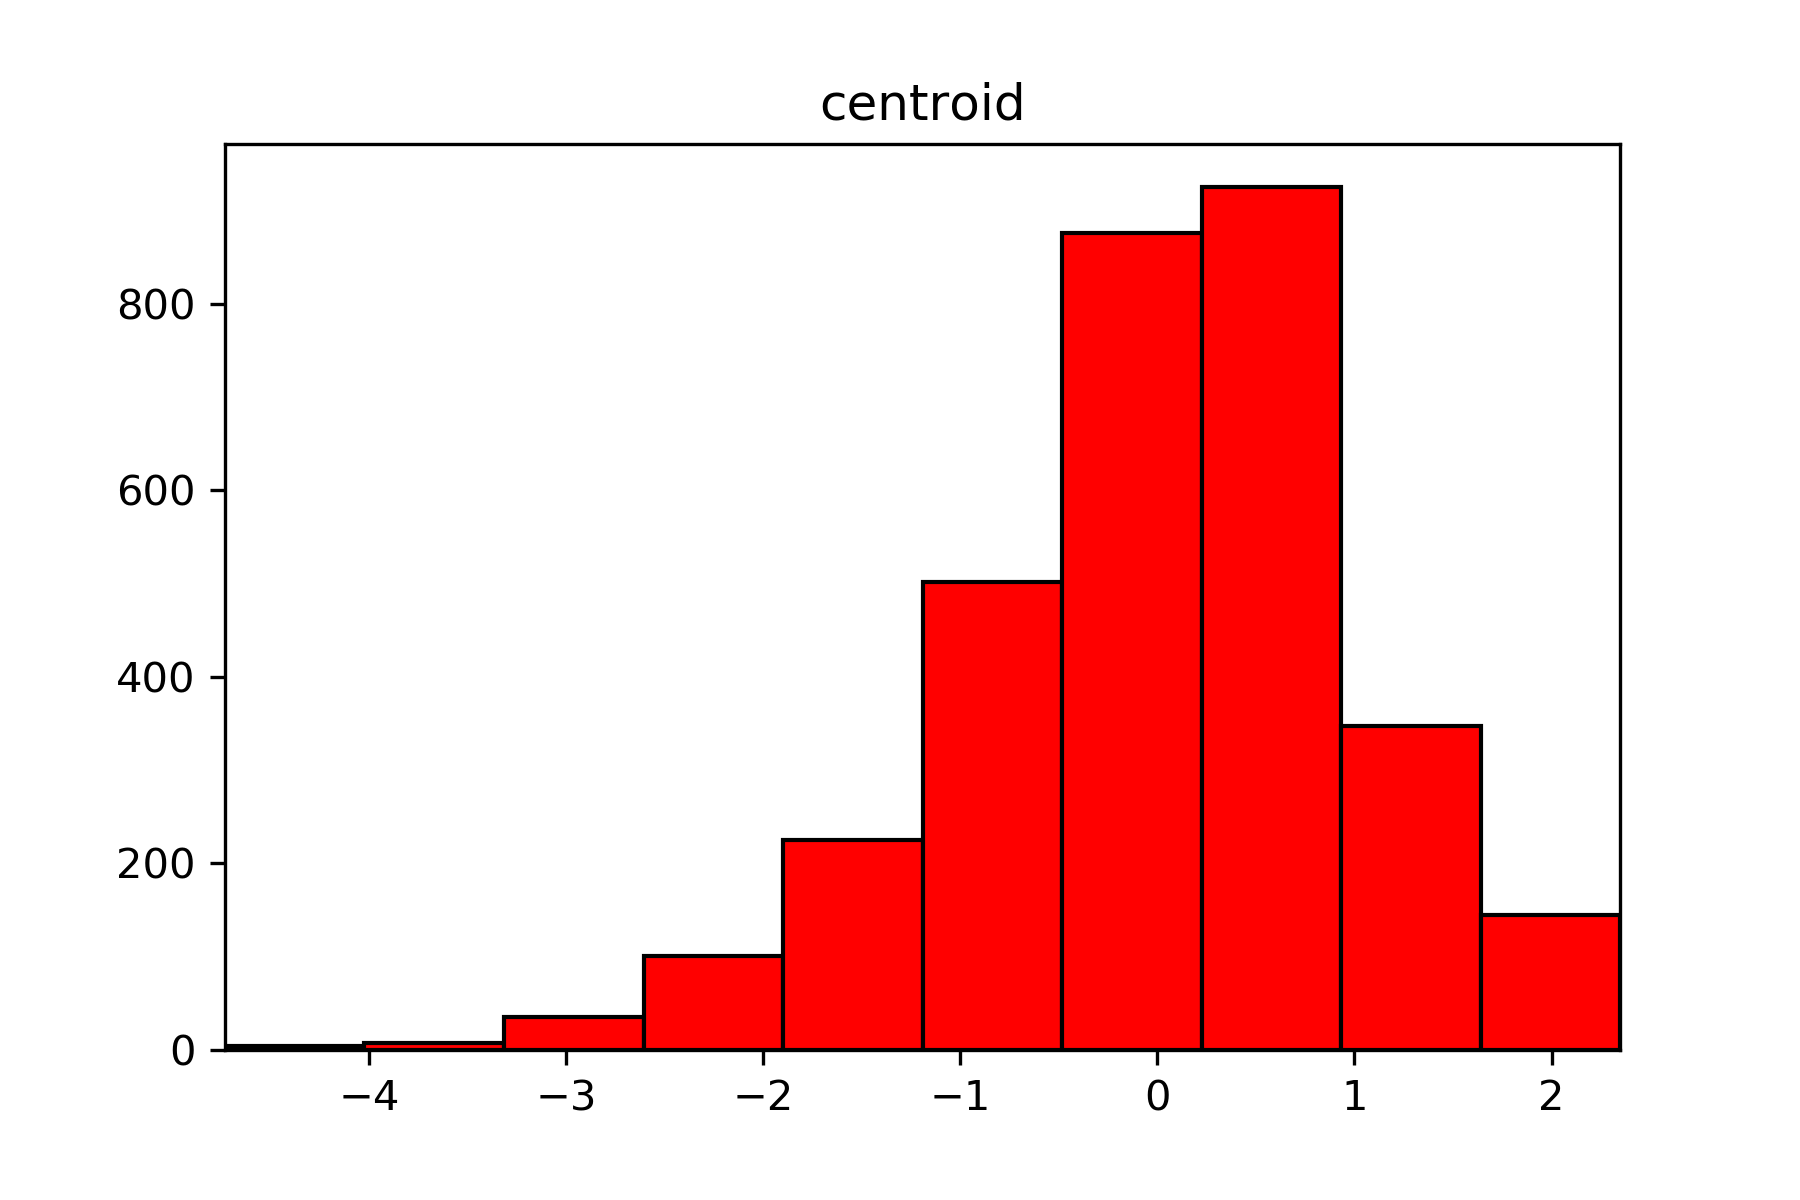
\includegraphics[width=3.85cm]{std_10_centroid}
        \caption{centroid}
        \label{fig:sub_std_11}
    \end{subfigure}\hfill
    % meanfun
    \begin{subfigure}{0.32\textwidth}
        \centering
        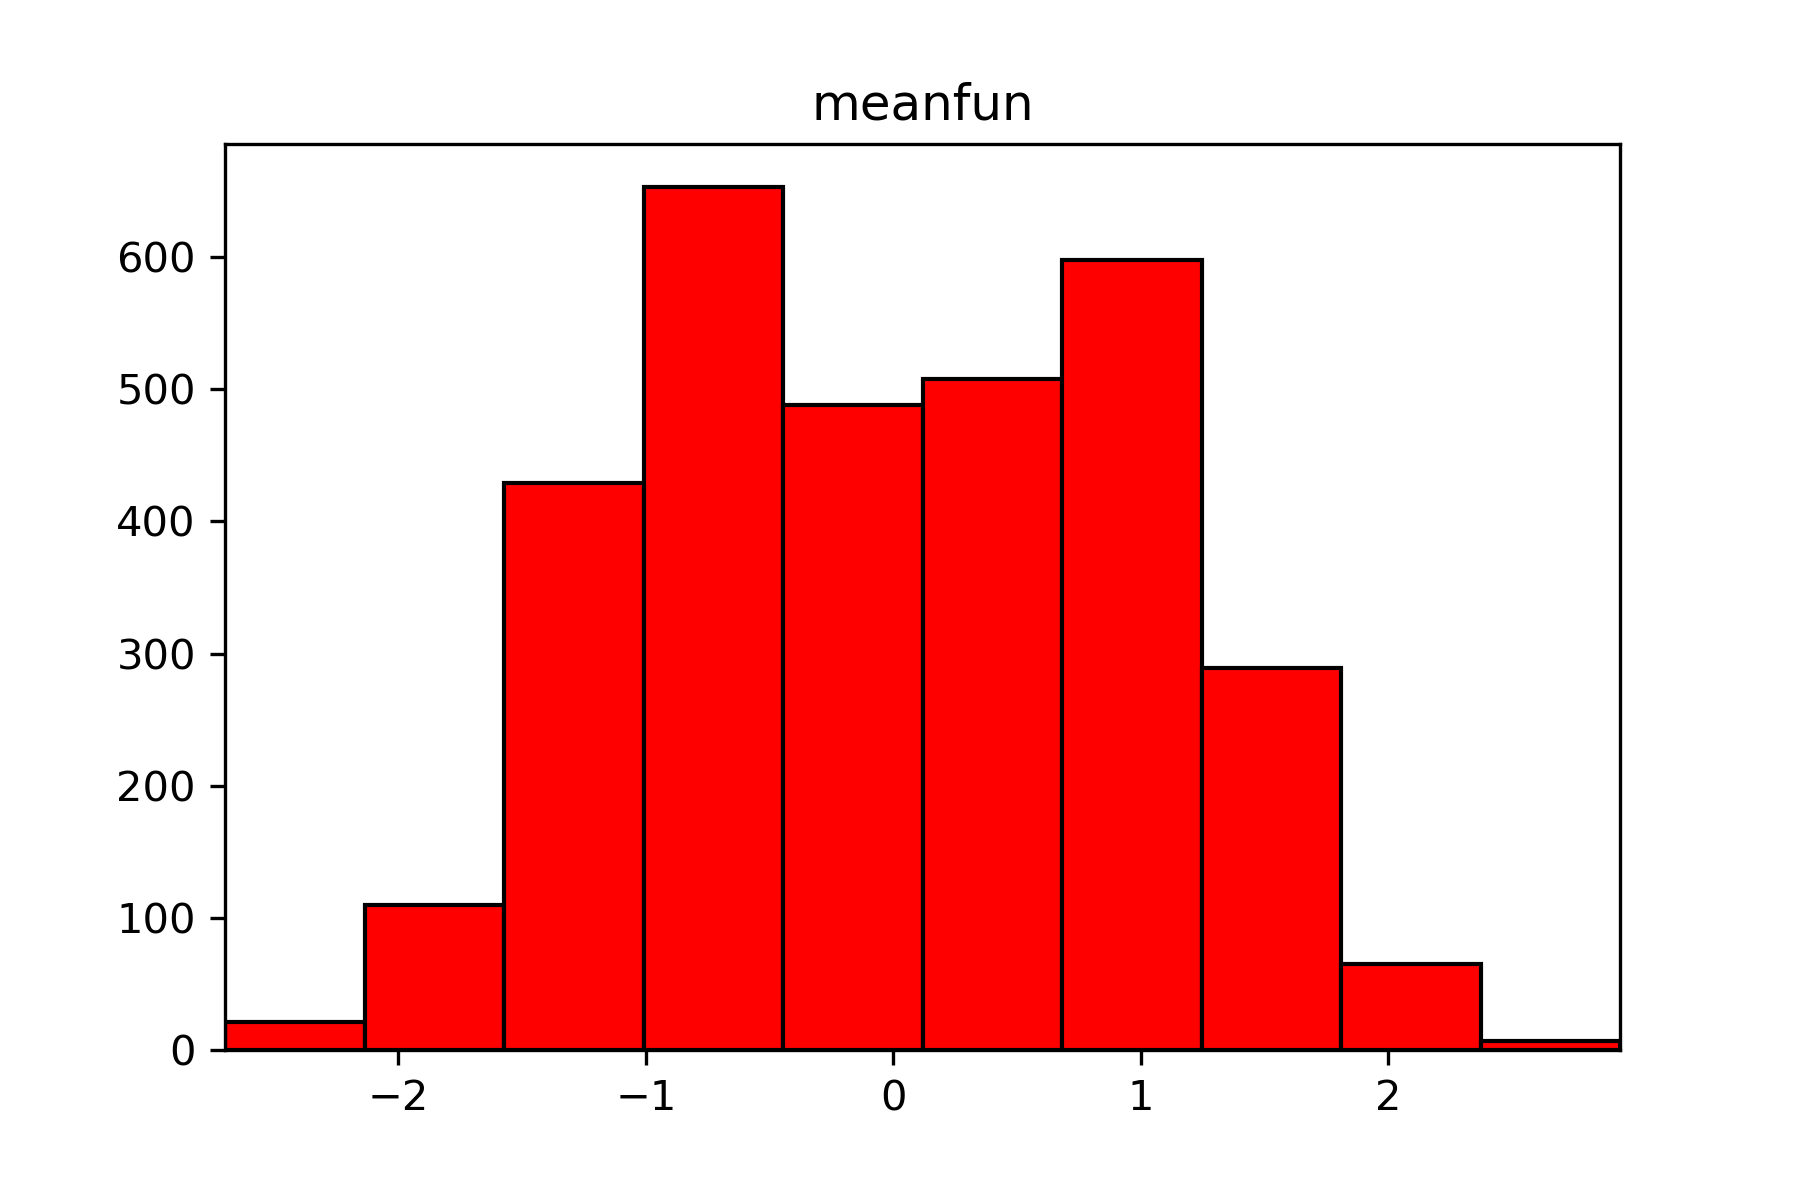
\includegraphics[width=3.85cm]{std_11_meanfun}
        \caption{meanfun}
        \label{fig:sub_std_12}
    \end{subfigure}\hfill
    % minfun
    \begin{subfigure}{0.32\textwidth}
        \centering
        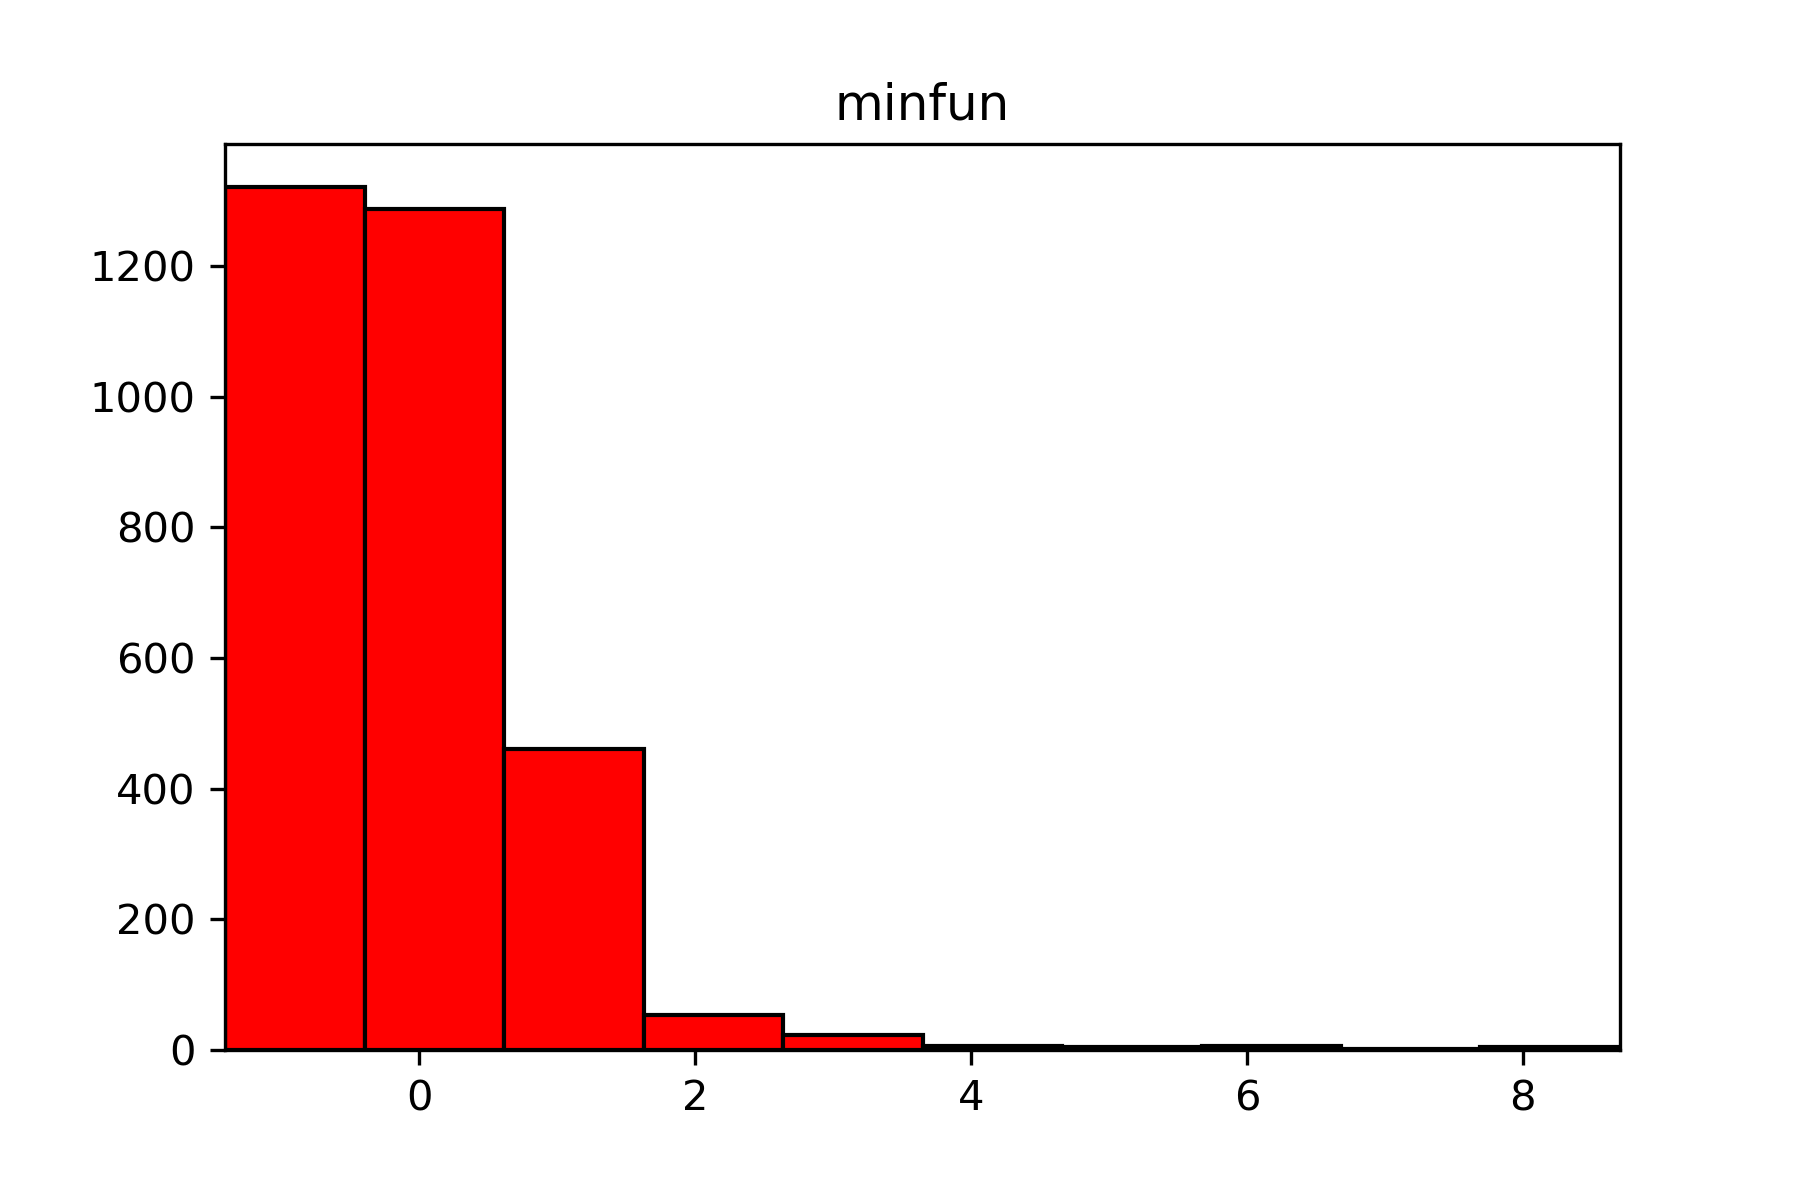
\includegraphics[width=3.85cm]{std_12_minfun}
        \caption{minfun}
        \label{fig:sub_std_13}
    \end{subfigure}\hfill
    % maxfun
    \begin{subfigure}{0.32\textwidth}
        \centering
        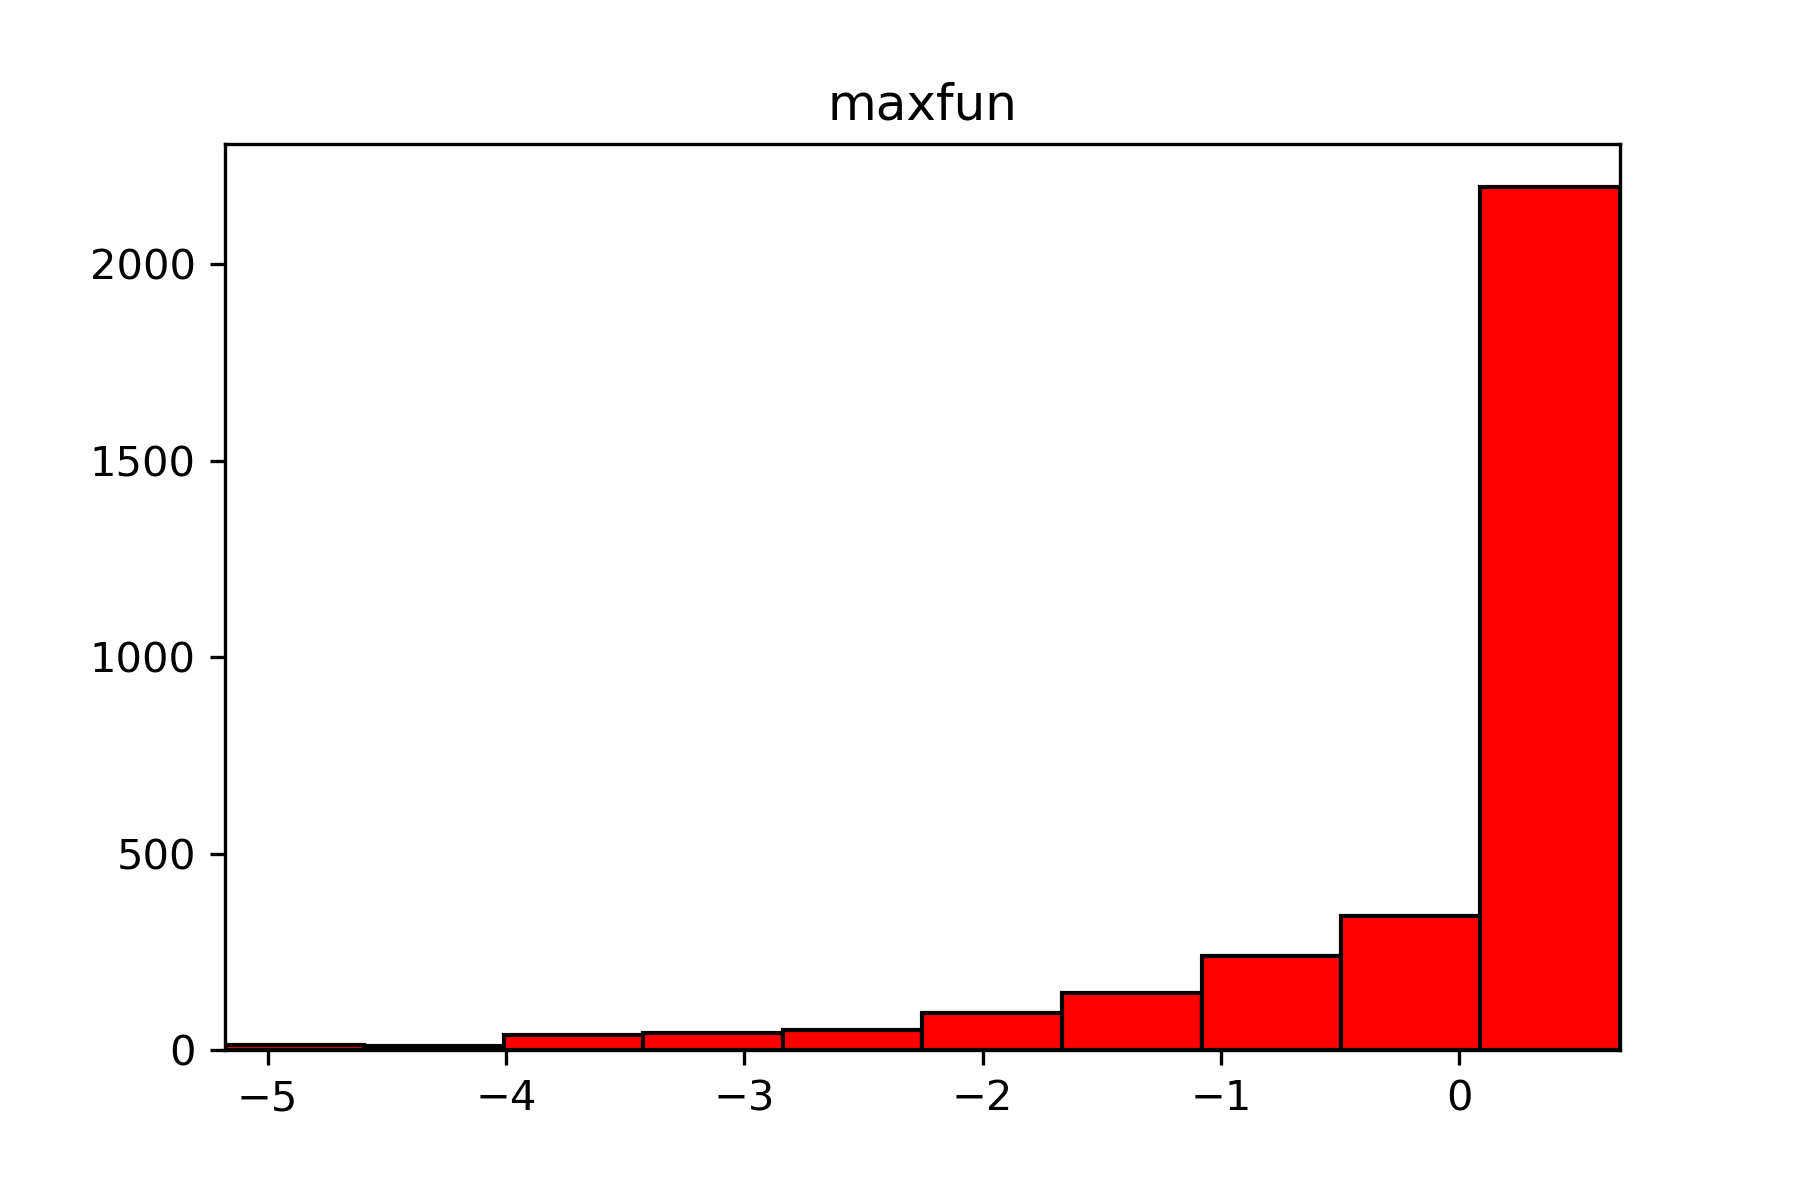
\includegraphics[width=3.85cm]{std_13_maxfun}
        \caption{maxfun}
        \label{fig:sub_std_14}
    \end{subfigure}\hfill
    % meandom
    \begin{subfigure}{0.32\textwidth}
        \centering
        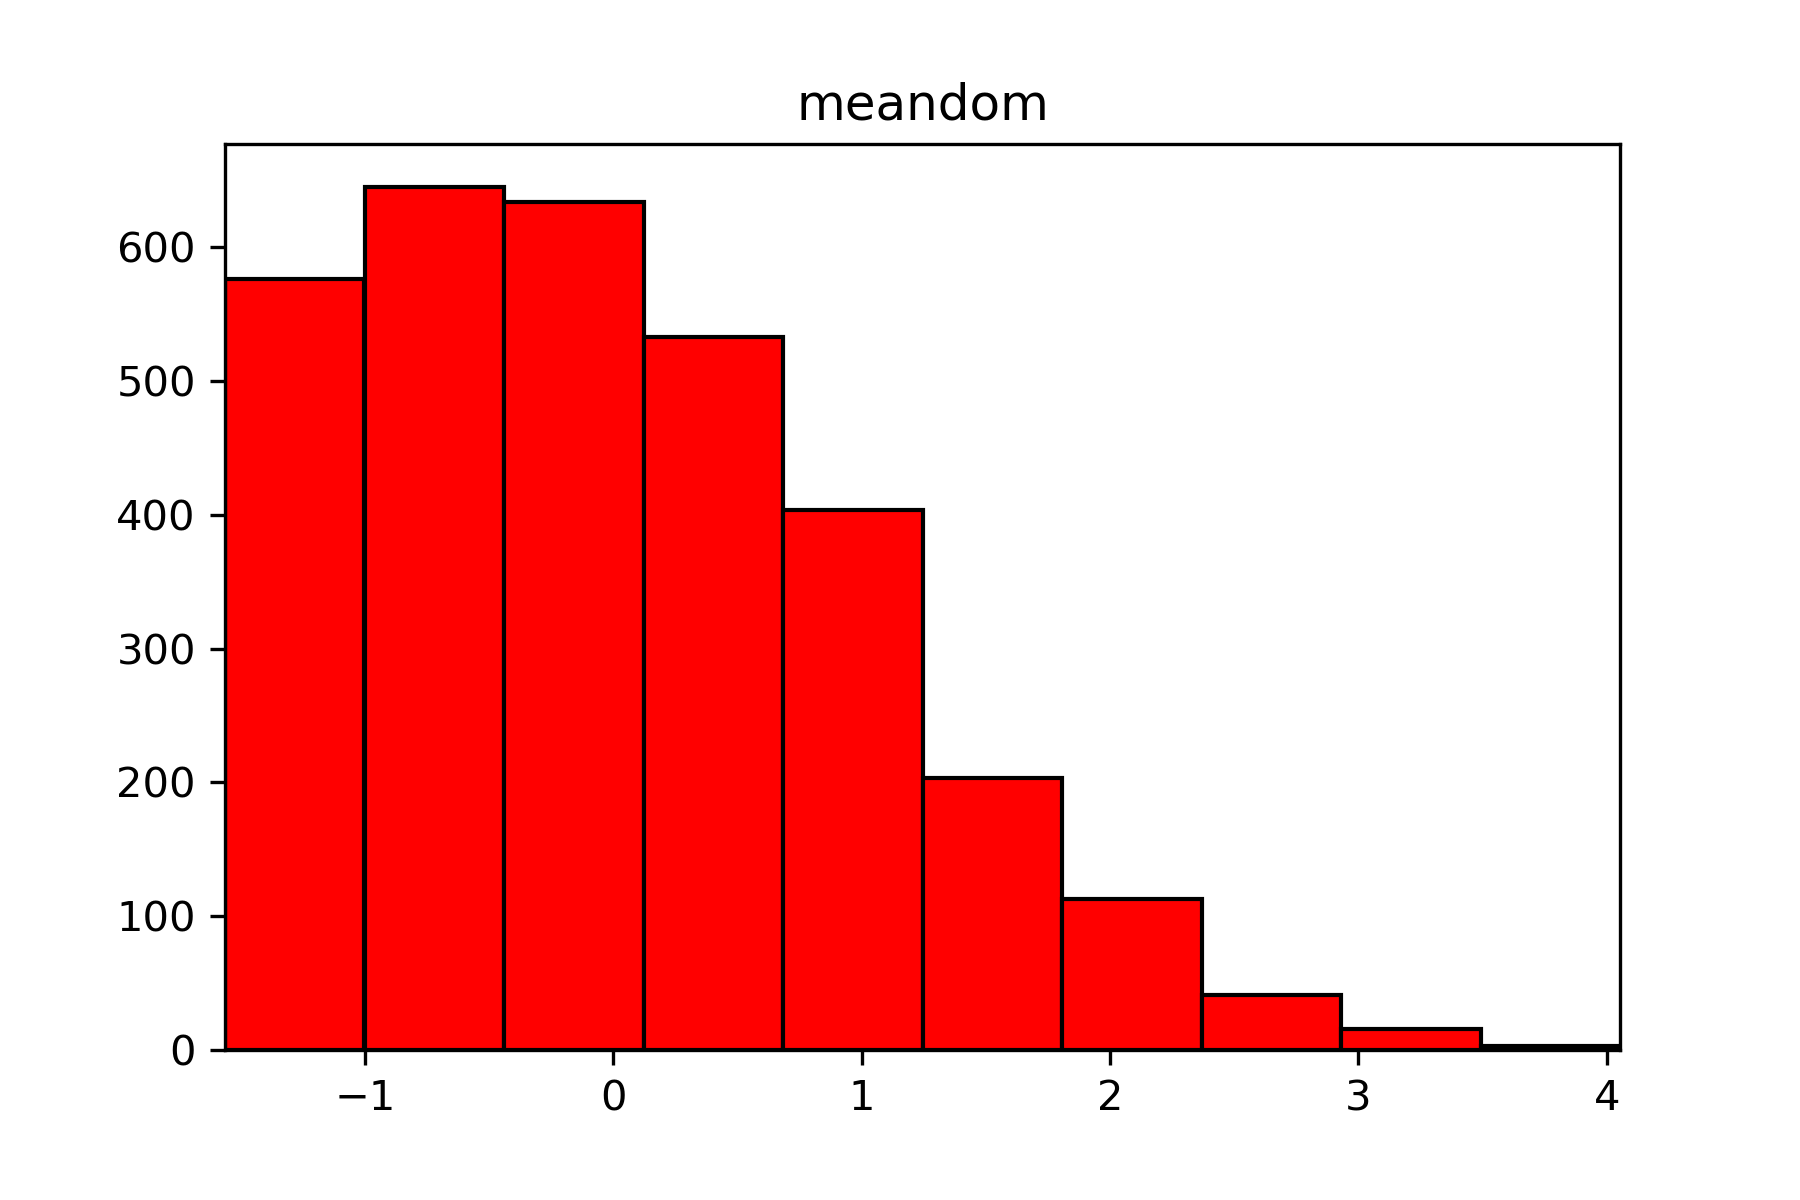
\includegraphics[width=3.85cm]{std_14_meandom}
        \caption{meandom}
        \label{fig:sub_std_15}
    \end{subfigure}\hfill
    % mindom
    \begin{subfigure}{0.32\textwidth}
        \centering
        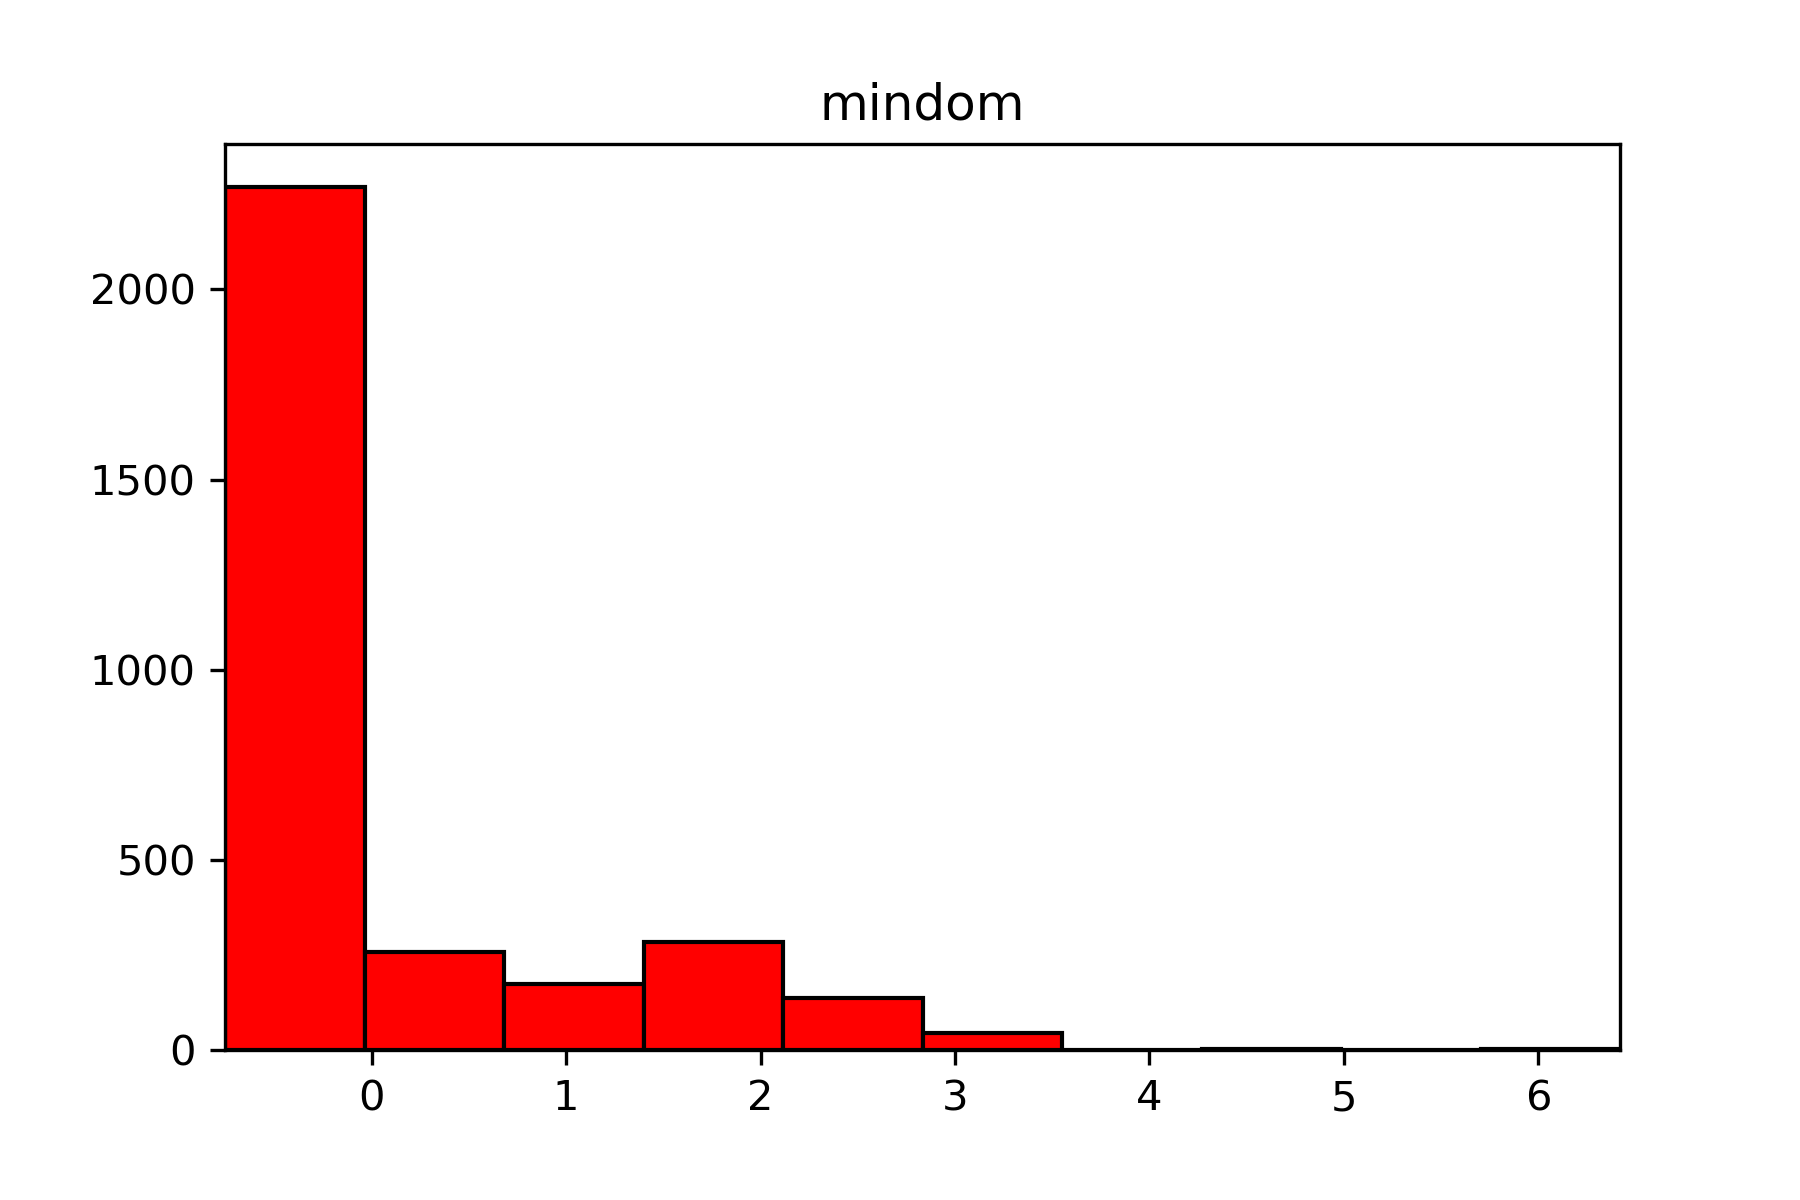
\includegraphics[width=3.85cm]{std_15_mindom}
        \caption{mindom}
        \label{fig:sub_std_16}
    \end{subfigure}\hfill
    % maxdom
    \begin{subfigure}{0.32\textwidth}
        \centering
        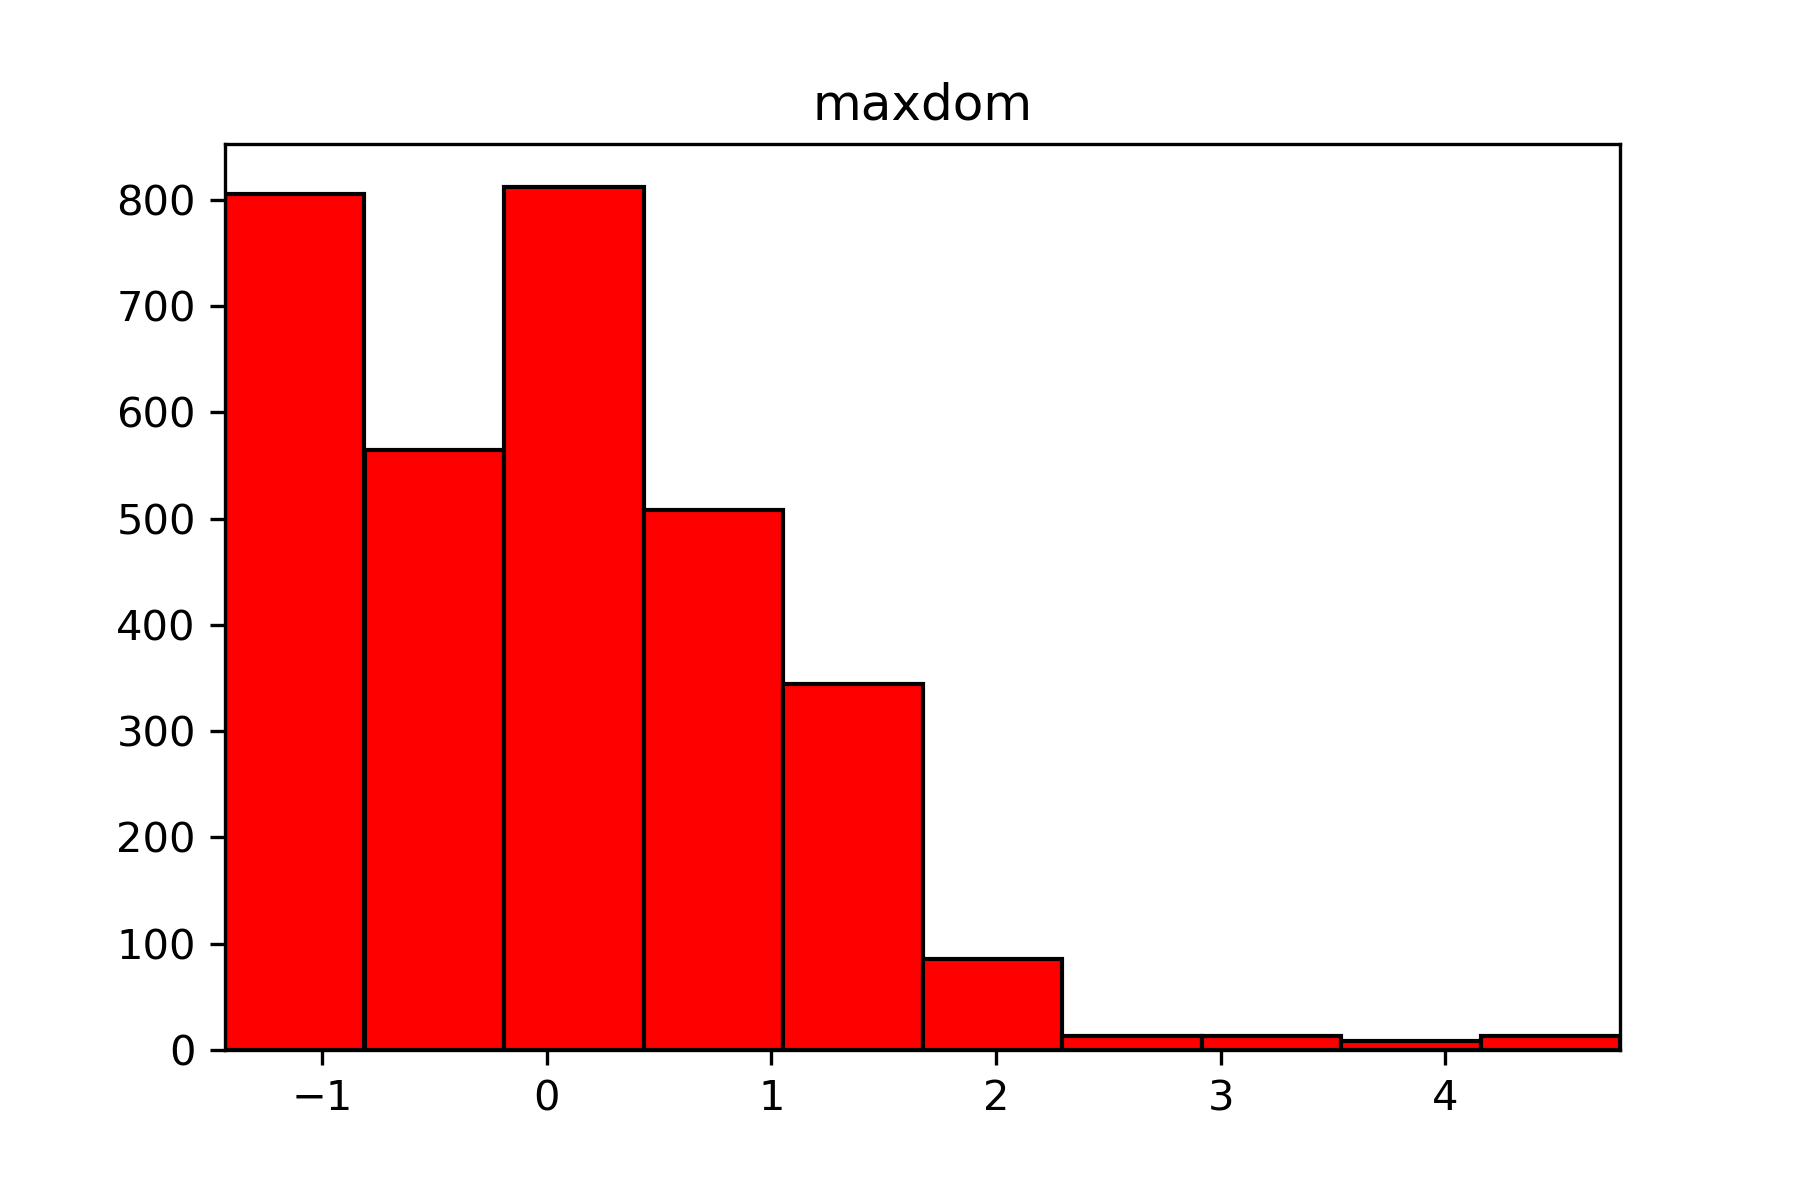
\includegraphics[width=3.85cm]{std_16_maxdom}
        \caption{maxdom}
        \label{fig:sub_std_17}
    \end{subfigure}\hfill
    % dfrange
    \begin{subfigure}{0.32\textwidth}
        \centering
        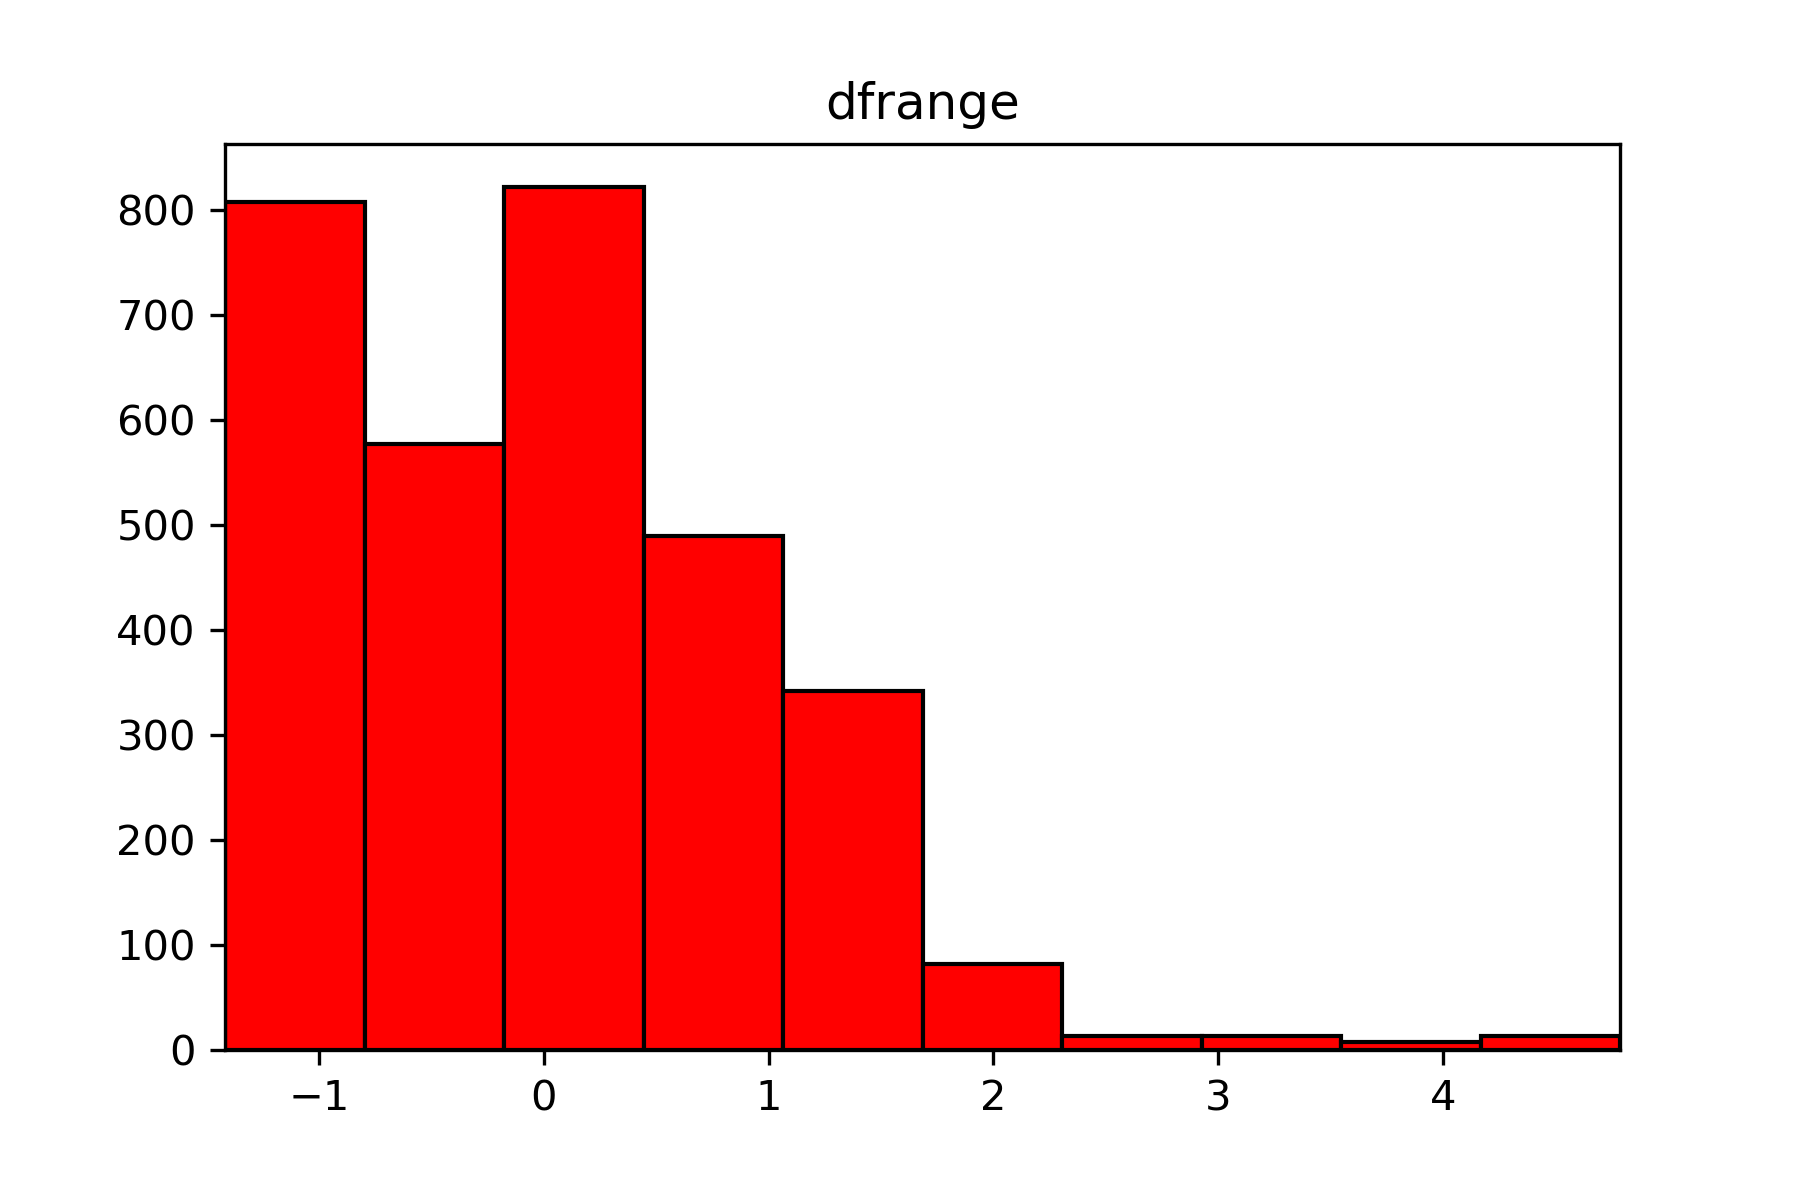
\includegraphics[width=3.85cm]{std_17_dfrange}
        \caption{dfrange}
        \label{fig:sub_std_18}
    \end{subfigure}\hfill
    % modindx
    \begin{subfigure}{0.32\textwidth}
        \centering
        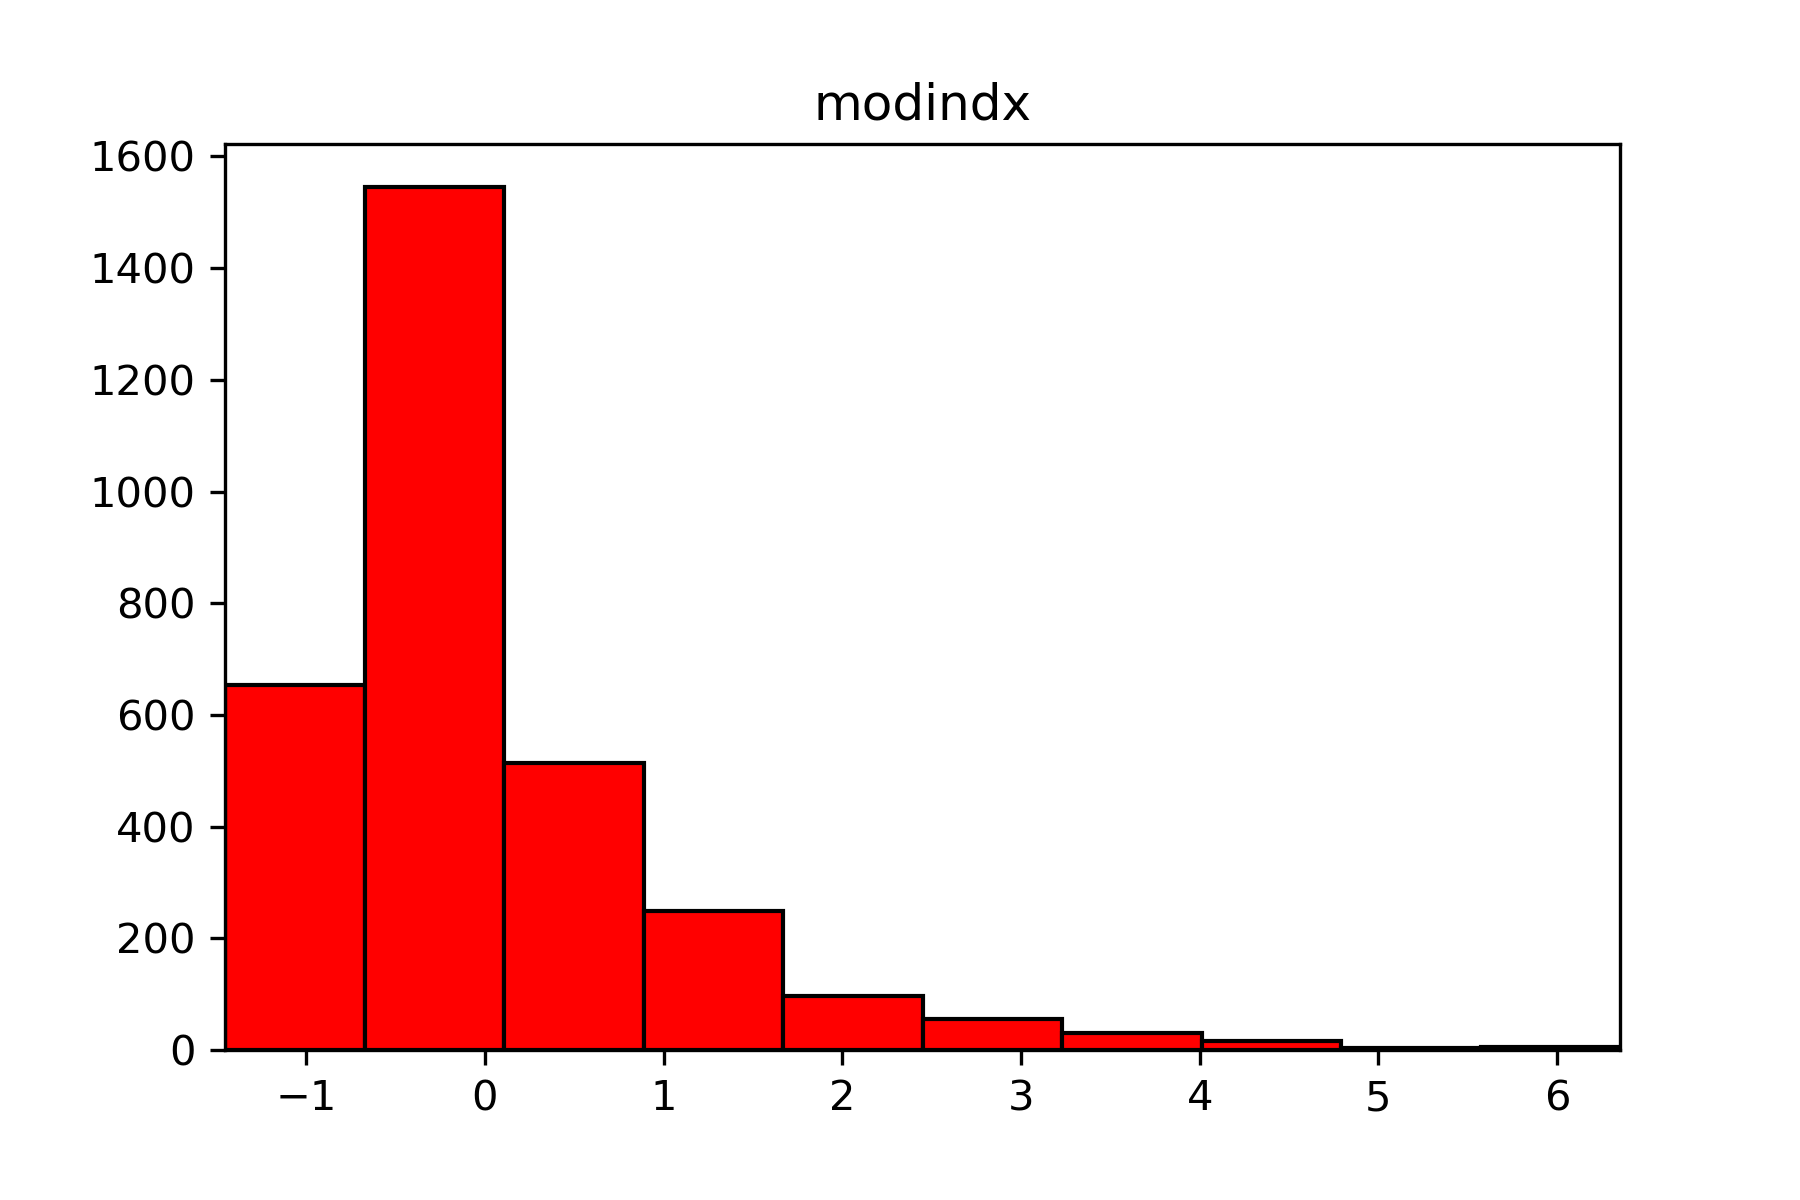
\includegraphics[width=3.85cm]{std_18_modindx}
        \caption{modindx}
        \label{fig:sub_std_19}
    \end{subfigure}
    % caption and label
    \caption{Histograms of input features after data standardization}
    \label{fig:pre-ex1-std_histograms}
\end{figure}

% histograms of features according to the labels side-by-side

\begin{figure}[H]
    \centering
    % sd
    \begin{subfigure}{0.32\textwidth}
        \centering
        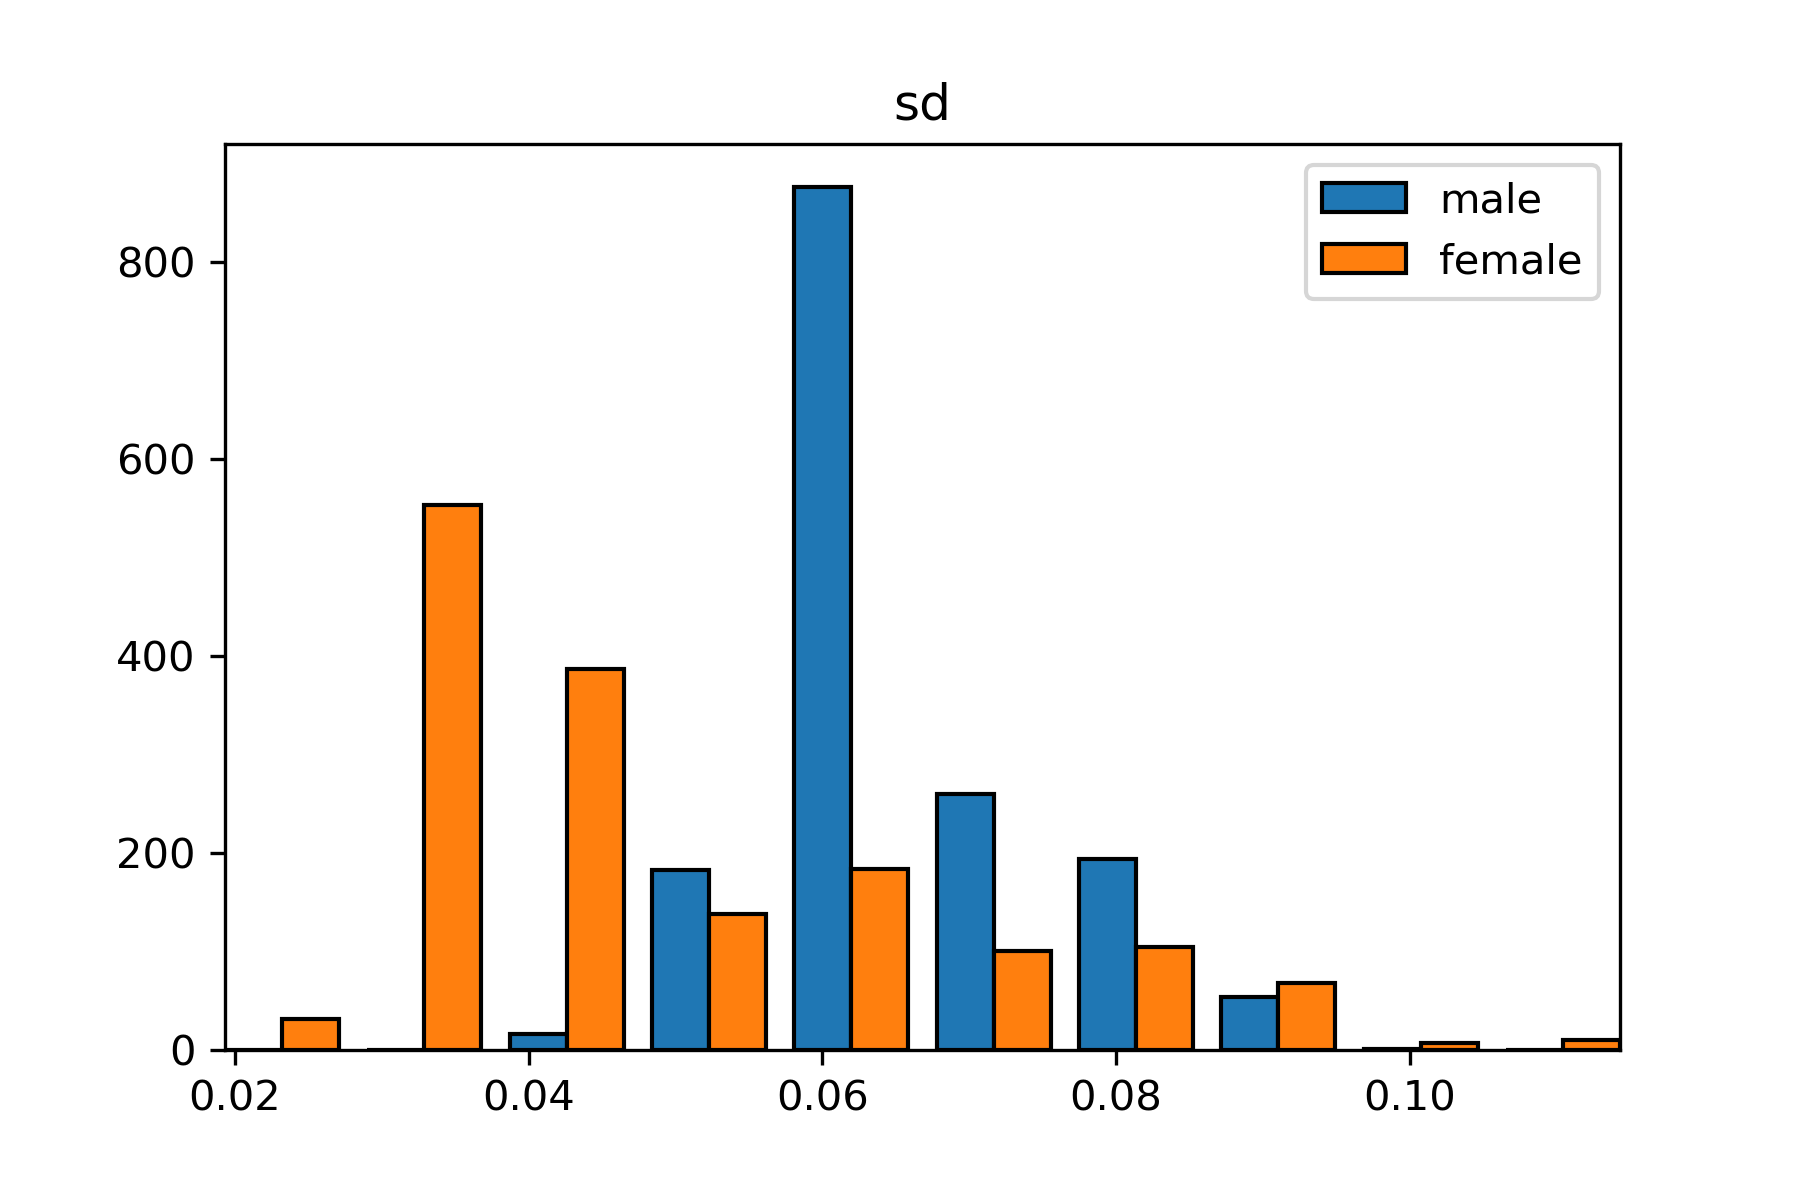
\includegraphics[width=3.85cm]{sbs_0_sd}
        \caption{sd}
        \label{fig:sub_sbs_1}
    \end{subfigure}
    \hfill
    % median
    \begin{subfigure}{0.32\textwidth}
        \centering
        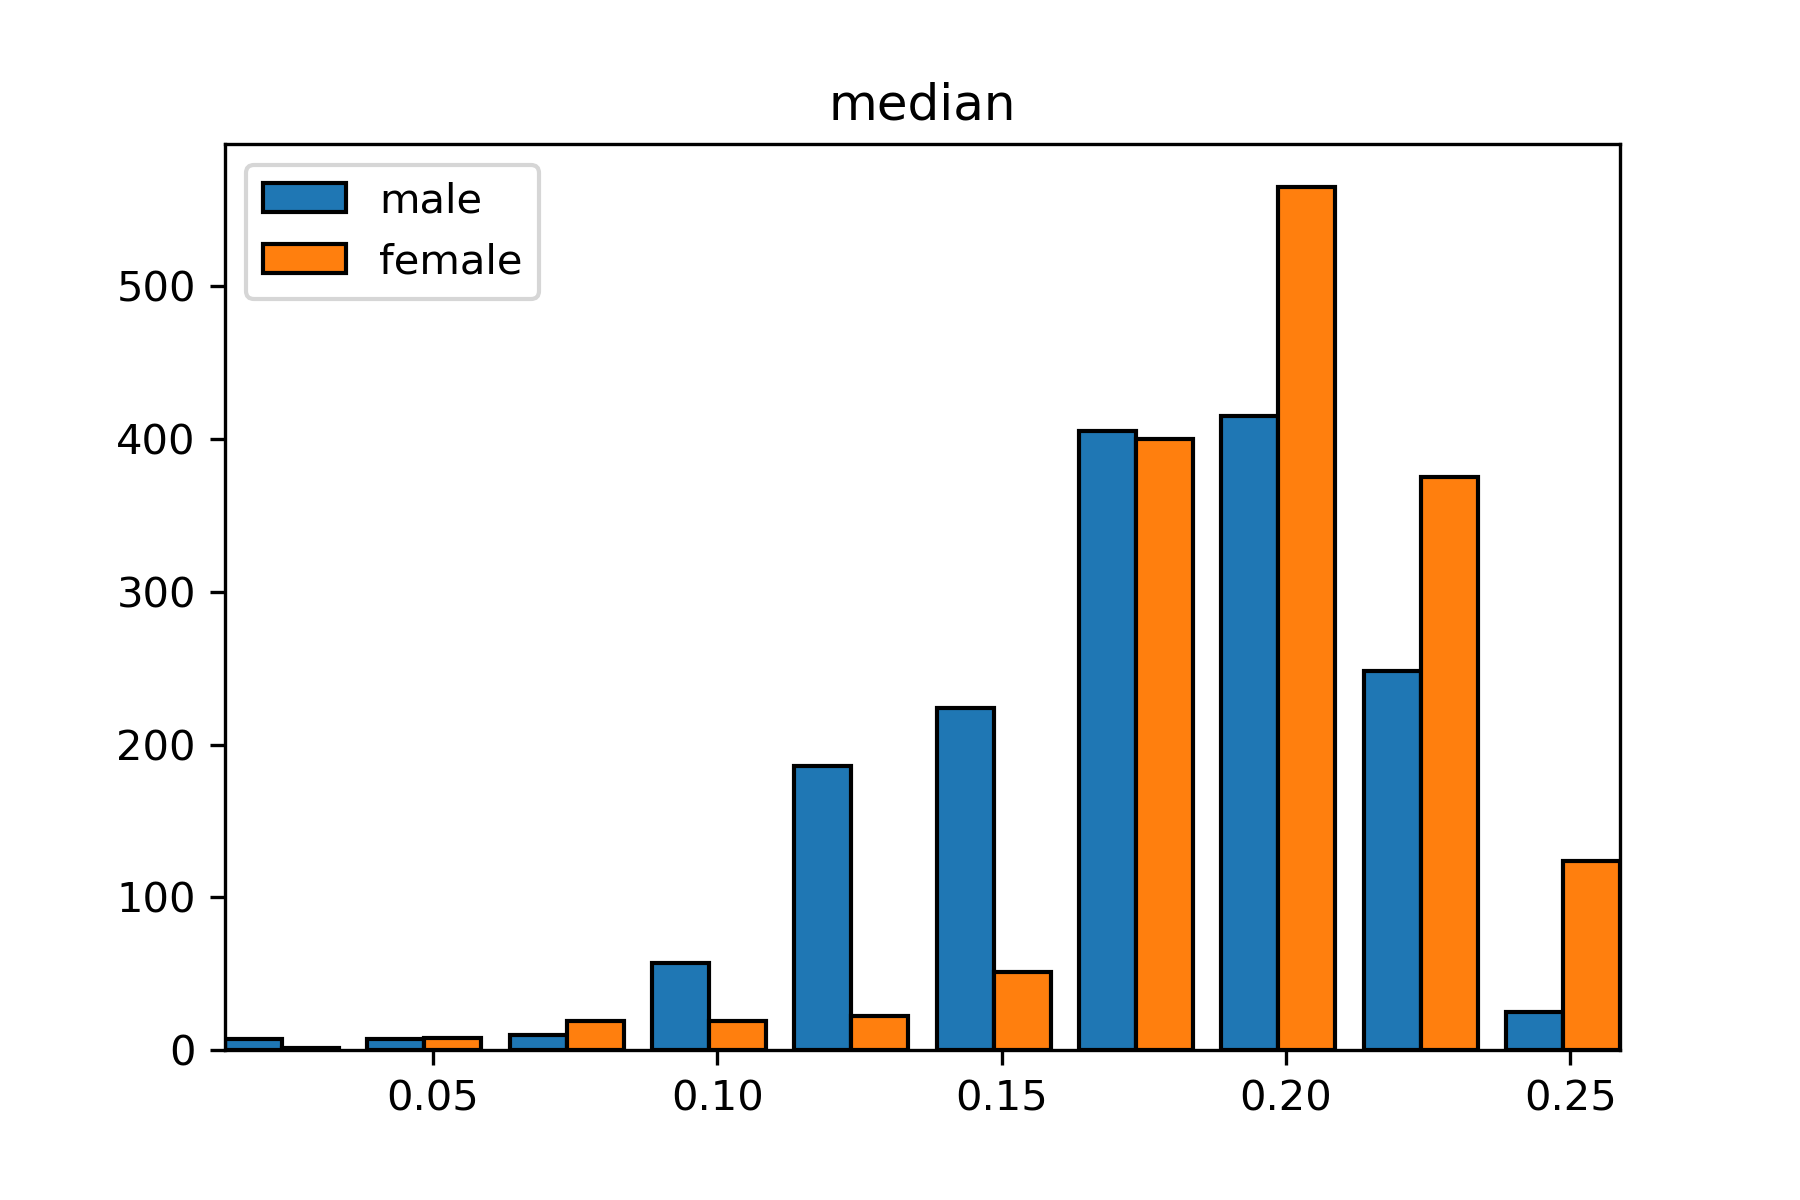
\includegraphics[width=3.85cm]{sbs_1_median}
        \caption{median}
        \label{fig:sub_sbs_2}
    \end{subfigure}
    \hfill
    % Q25
    \begin{subfigure}{0.32\textwidth}
        \centering
        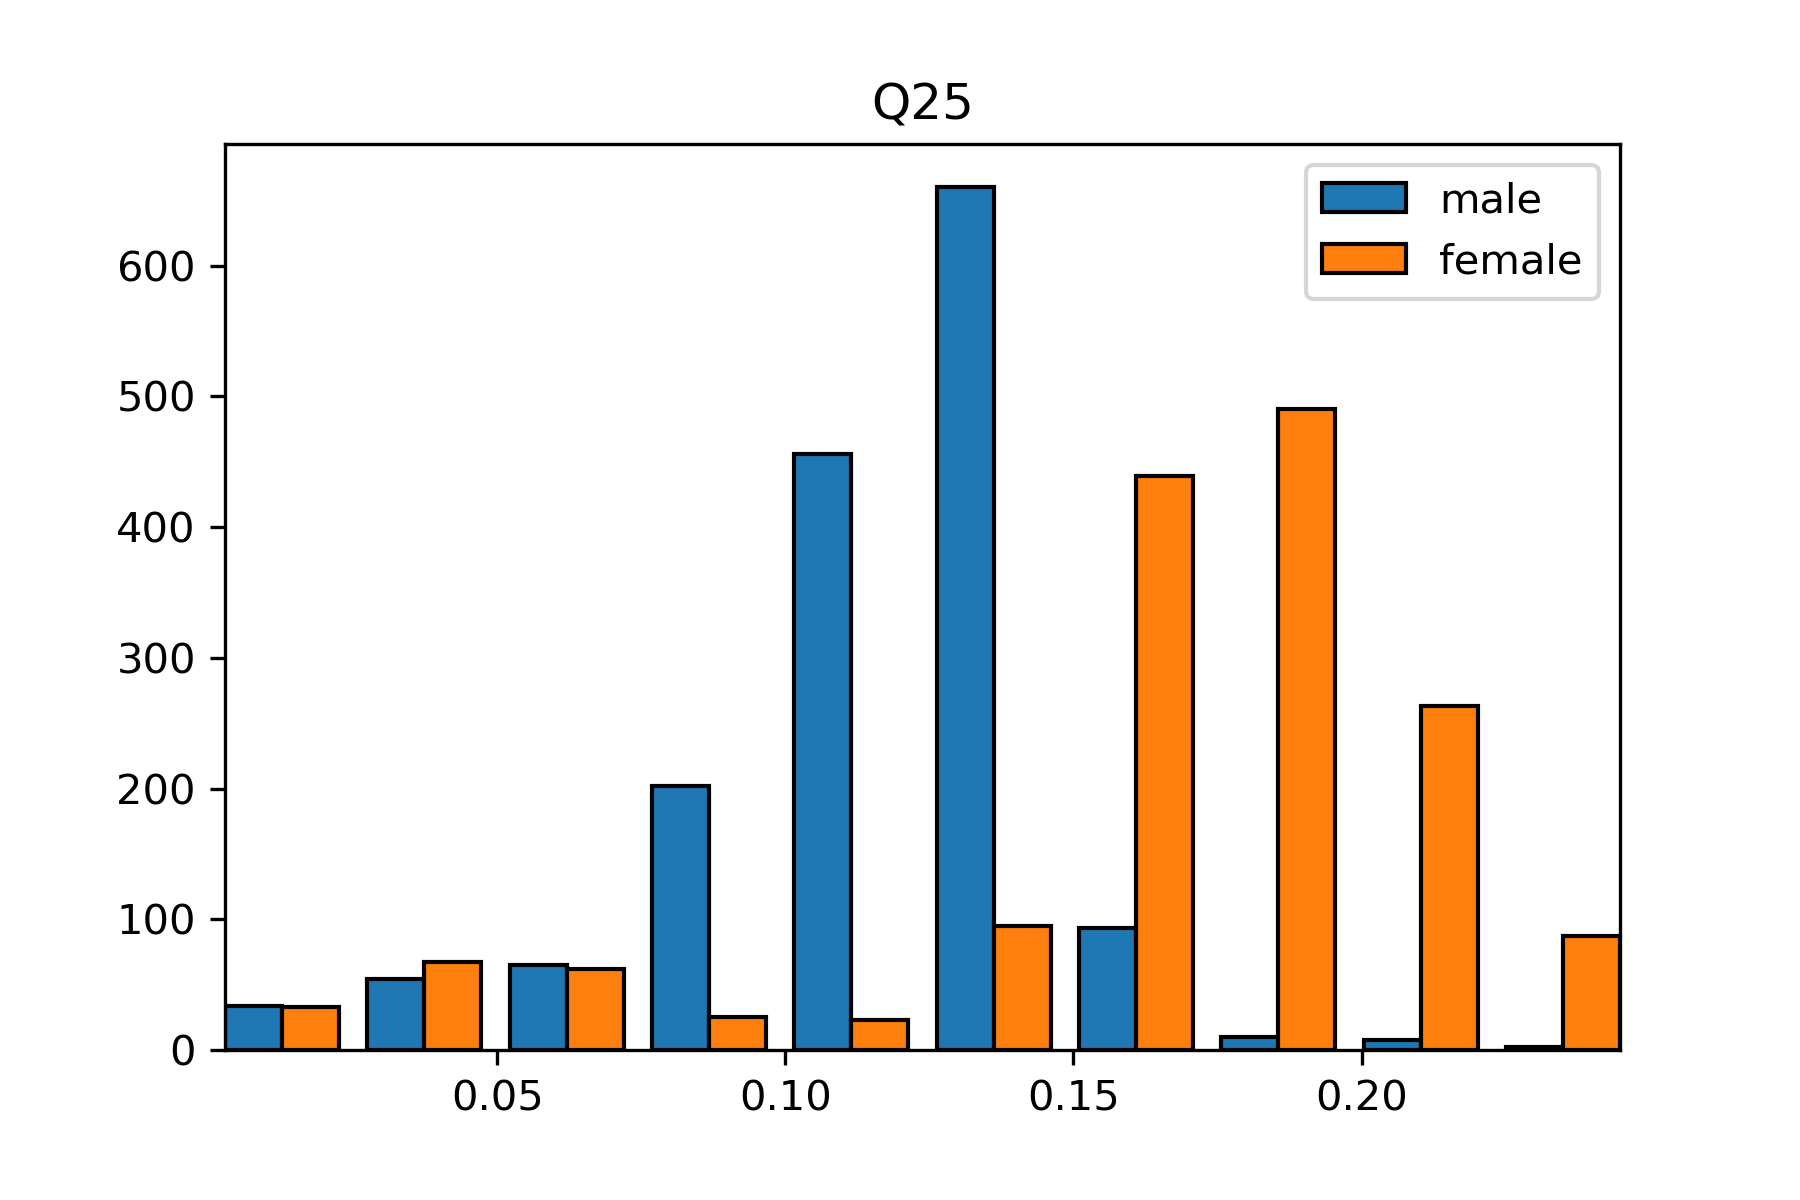
\includegraphics[width=3.85cm]{sbs_2_Q25}
        \caption{Q25}
        \label{fig:sub_sbs_3}
    \end{subfigure}%
    \\
    % Q75
    \begin{subfigure}{0.32\textwidth}
        \centering
        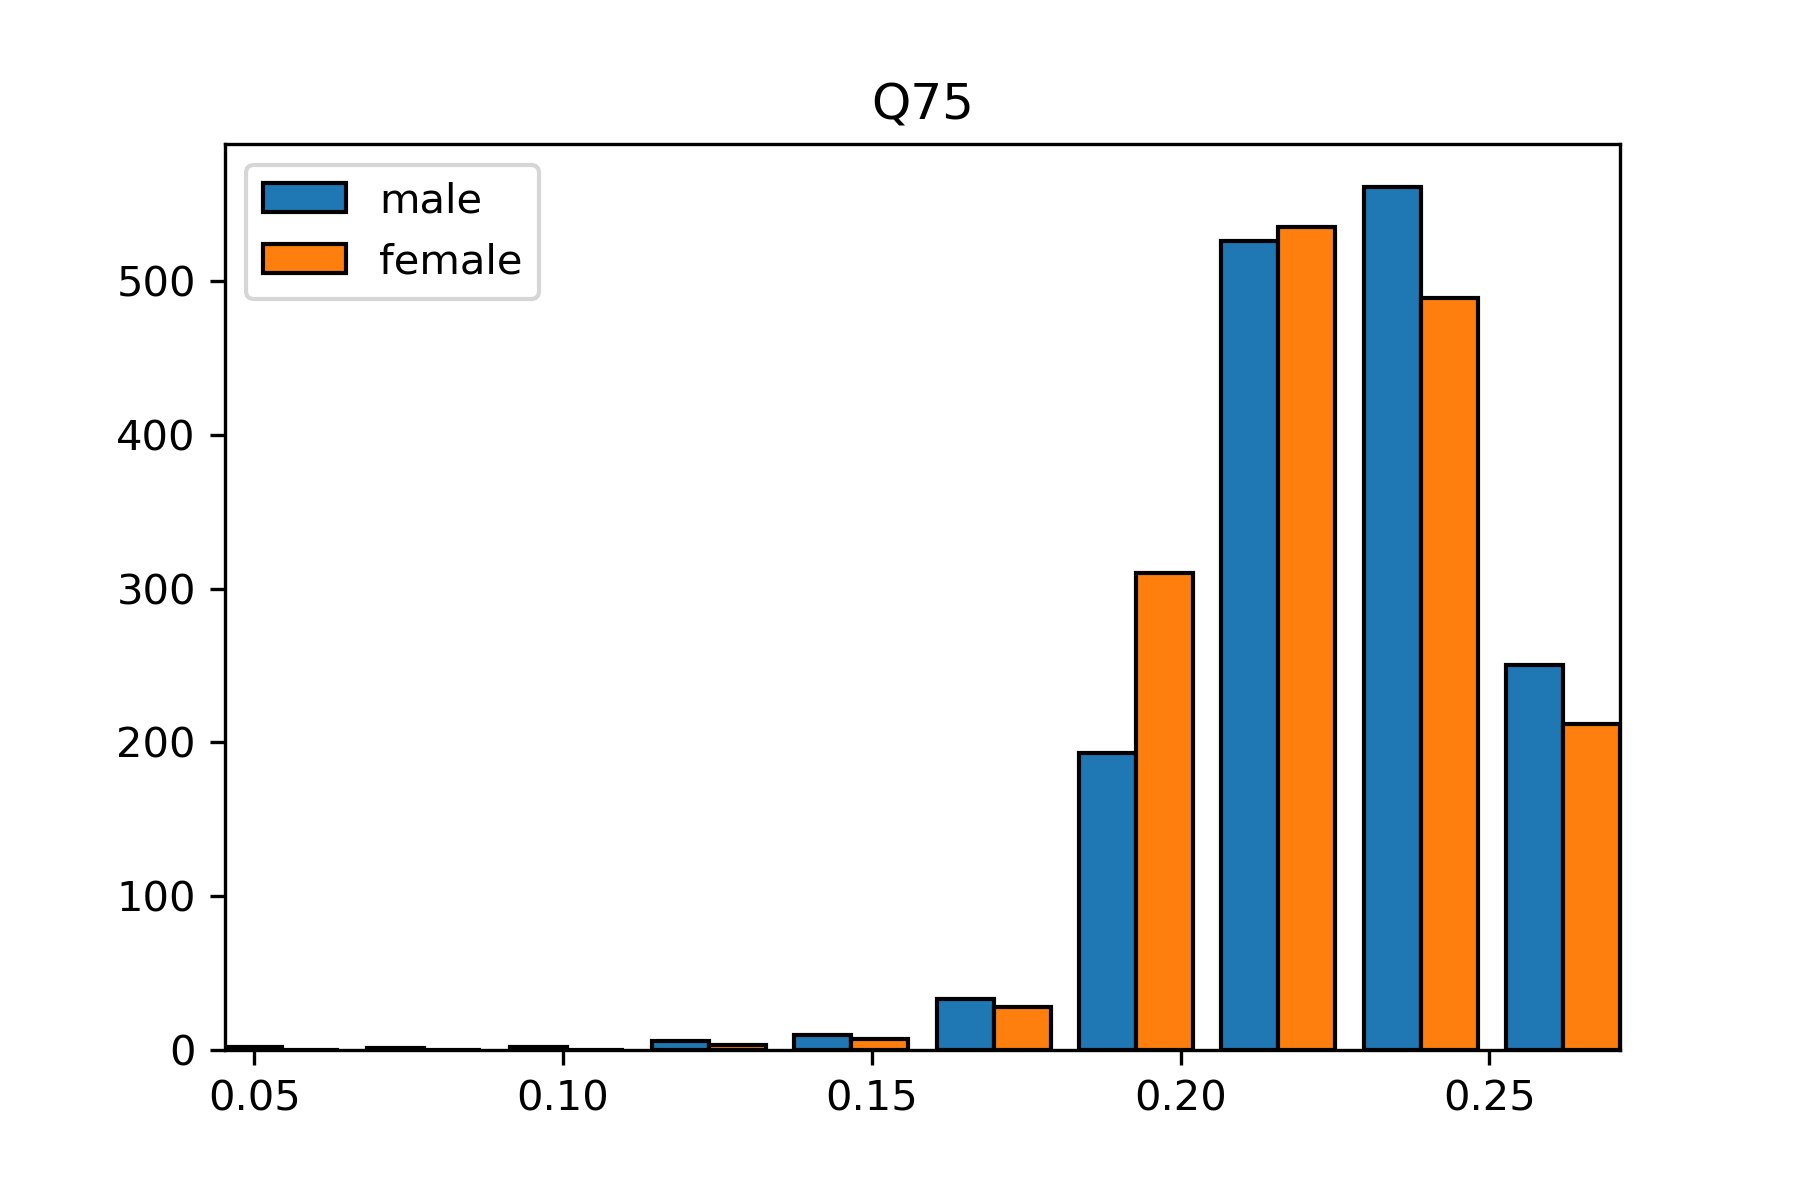
\includegraphics[width=3.85cm]{sbs_3_Q75}
        \caption{Q75}
        \label{fig:sub_sbs_4}
    \end{subfigure}\hfill
    % Q75
    \begin{subfigure}{0.32\textwidth}
        \centering
        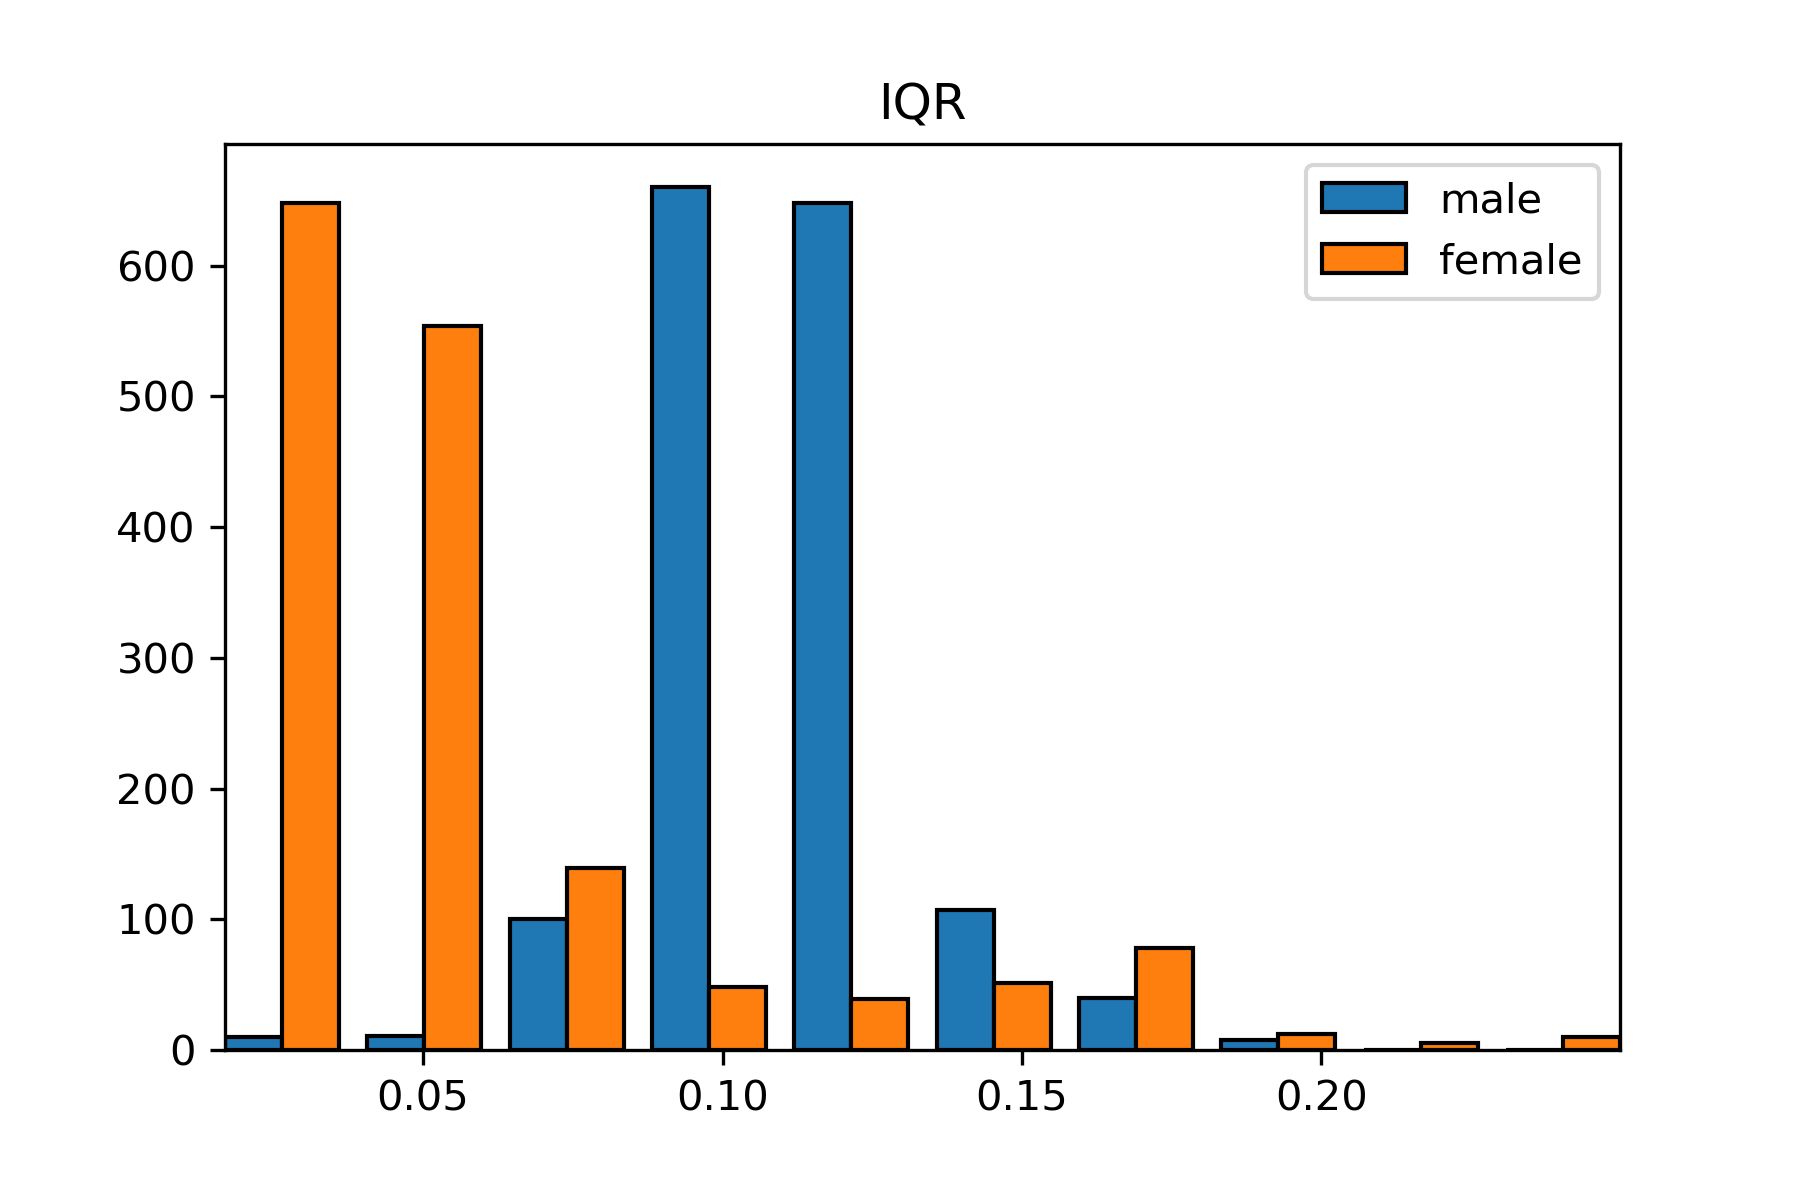
\includegraphics[width=3.85cm]{sbs_4_IQR}
        \caption{IQR}
        \label{fig:sub_sbs_5}
    \end{subfigure}\hfill
    % skew
    \begin{subfigure}{0.32\textwidth}
        \centering
        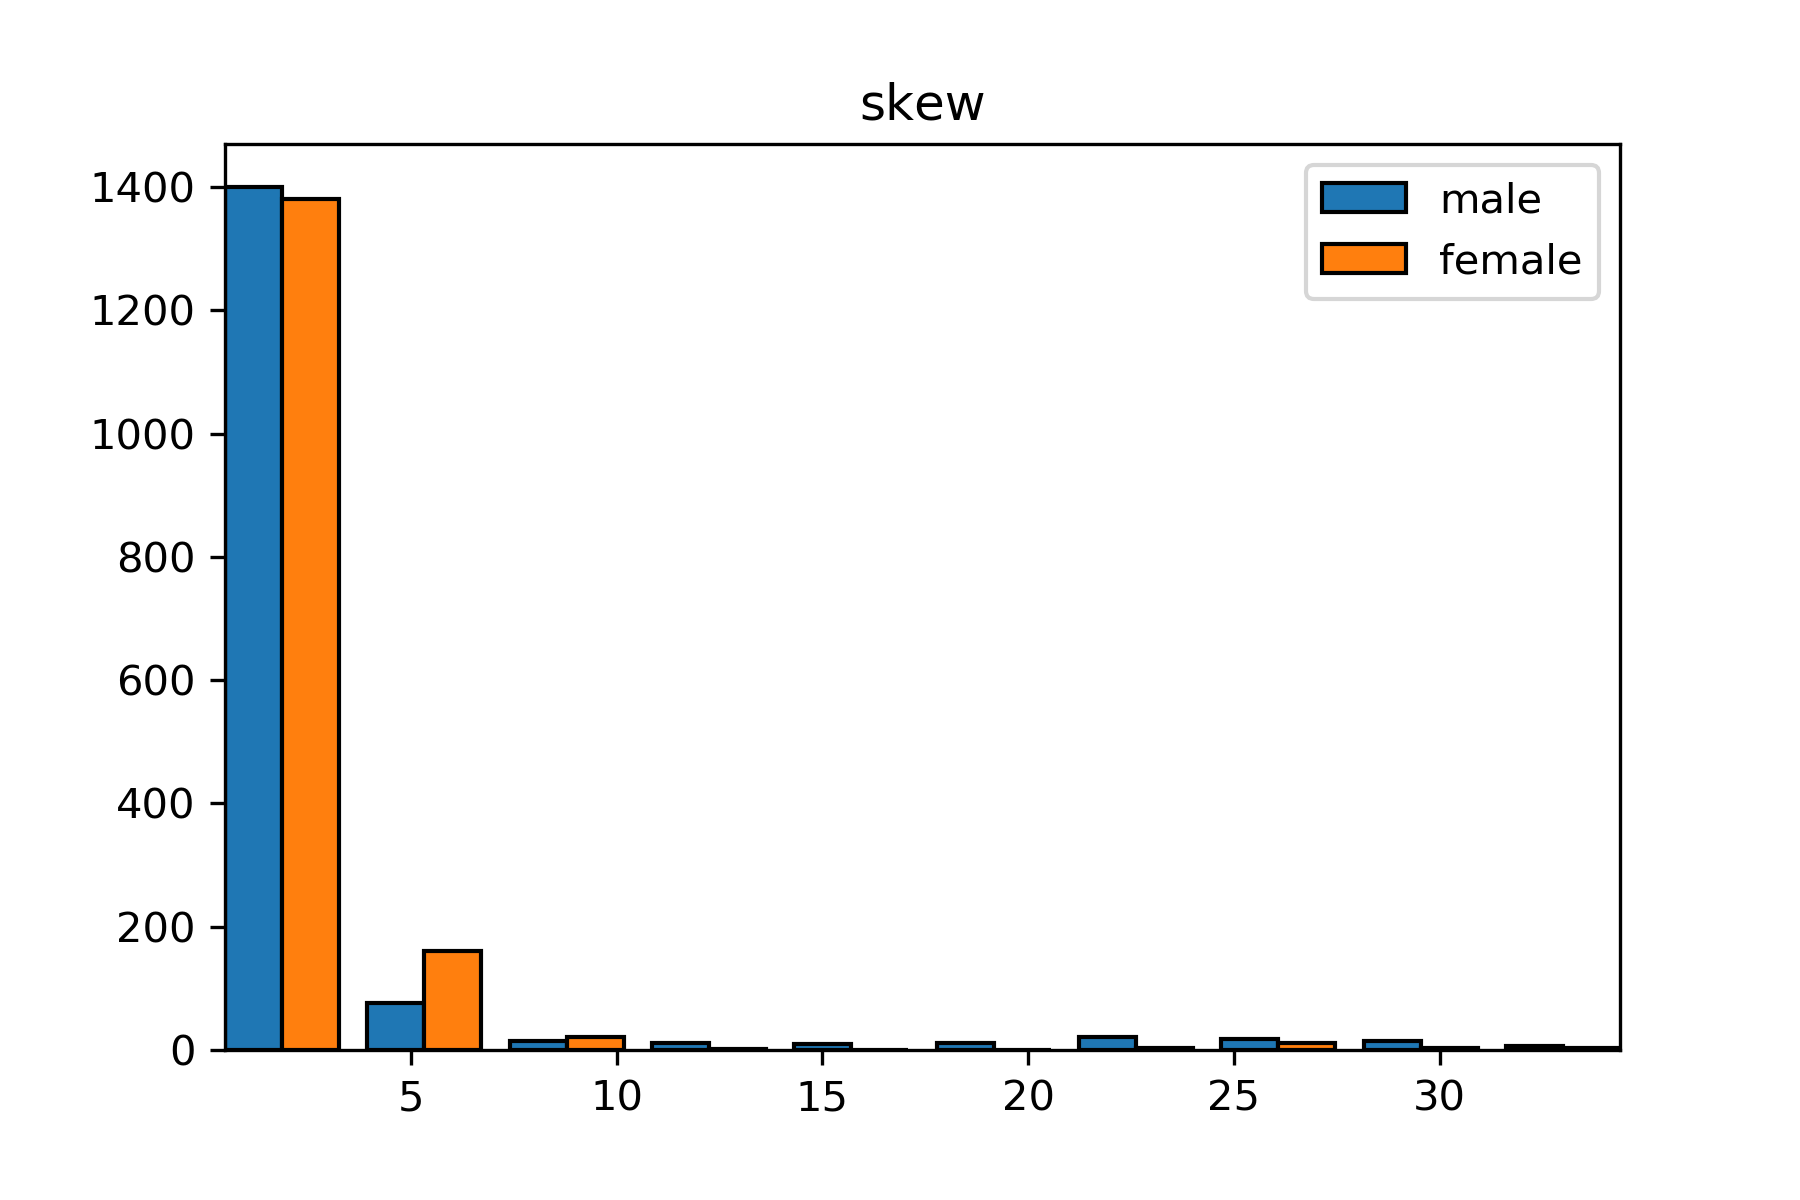
\includegraphics[width=3.85cm]{sbs_5_skew}
        \caption{skew}
        \label{fig:sub_sbs_6}
    \end{subfigure}
    \\
    % kurt
    \begin{subfigure}{0.32\textwidth}
        \centering
        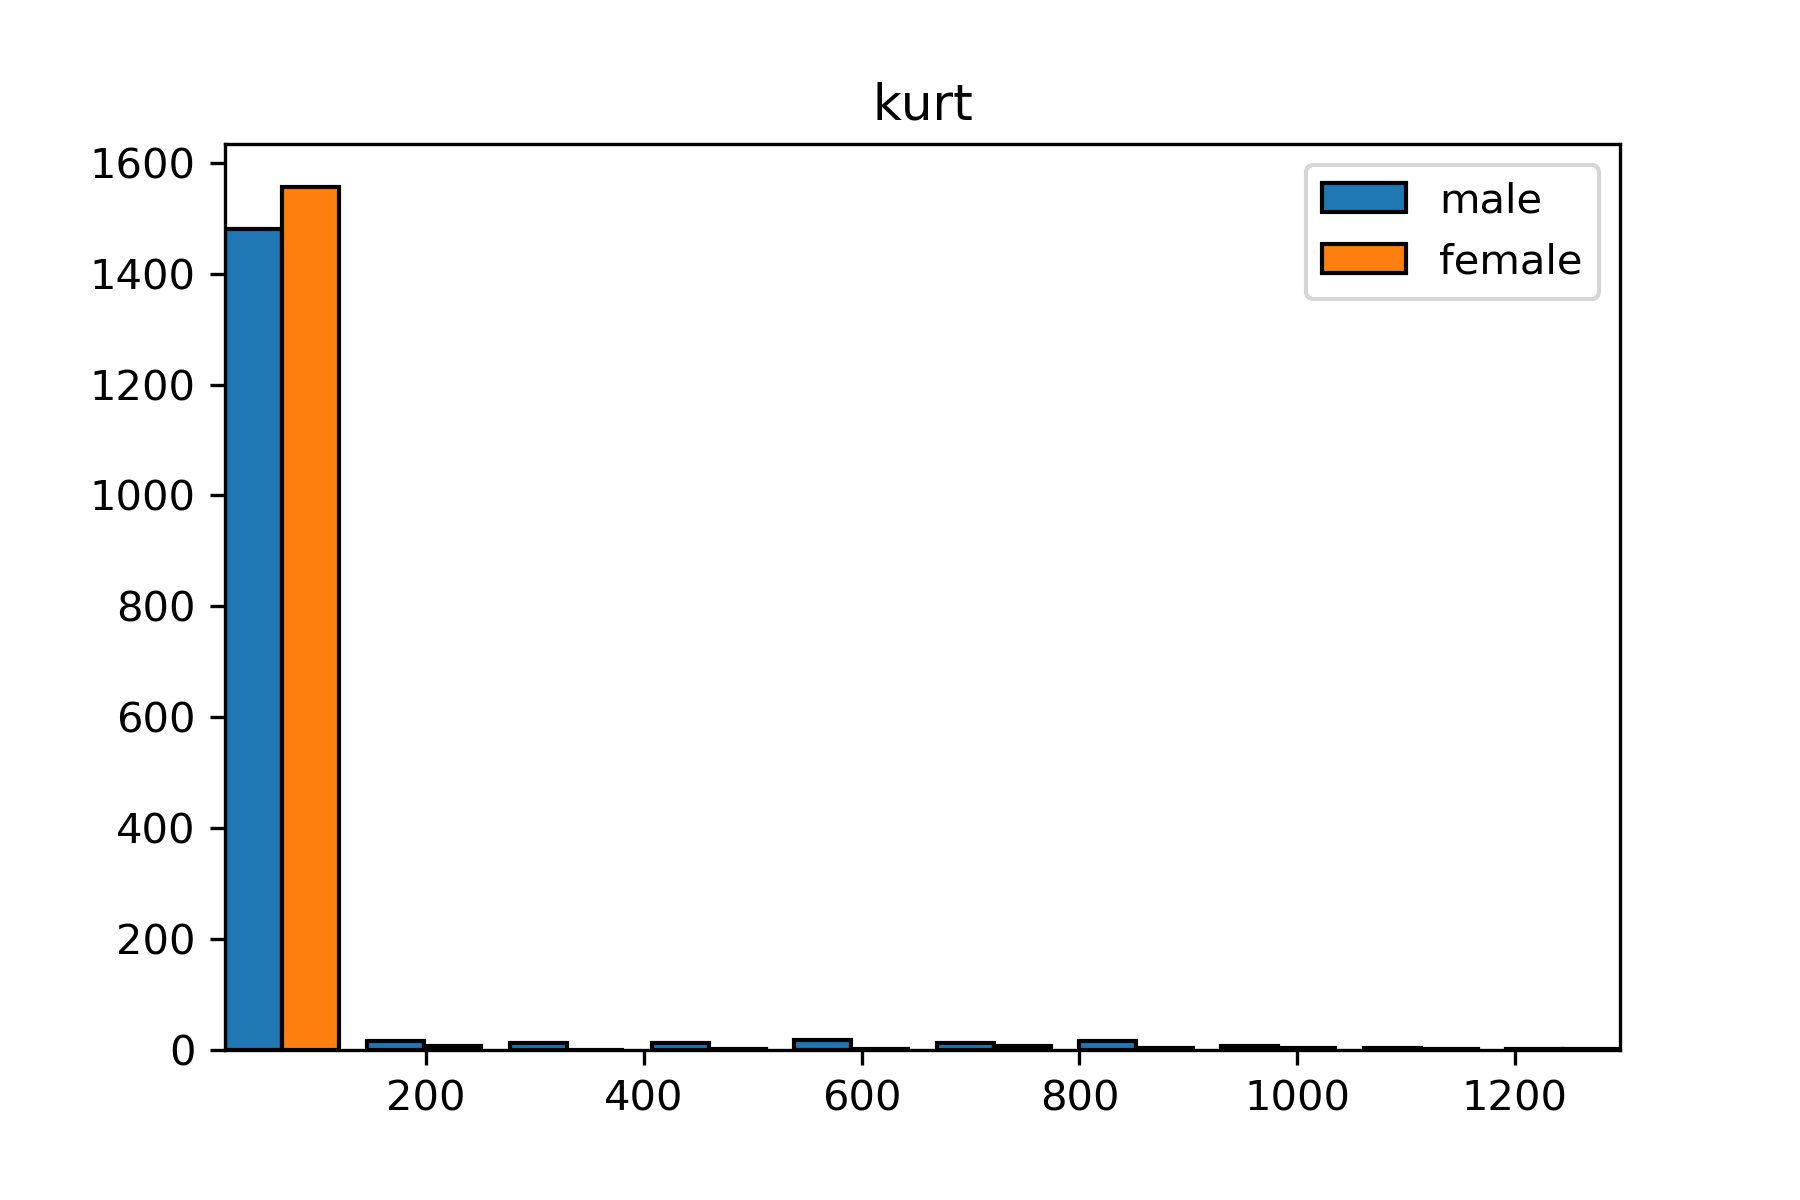
\includegraphics[width=3.85cm]{sbs_6_kurt}
        \caption{kurt}
        \label{fig:sub_sbs_7}
    \end{subfigure}\hfill
    % sp ent
    \begin{subfigure}{0.32\textwidth}
        \centering
        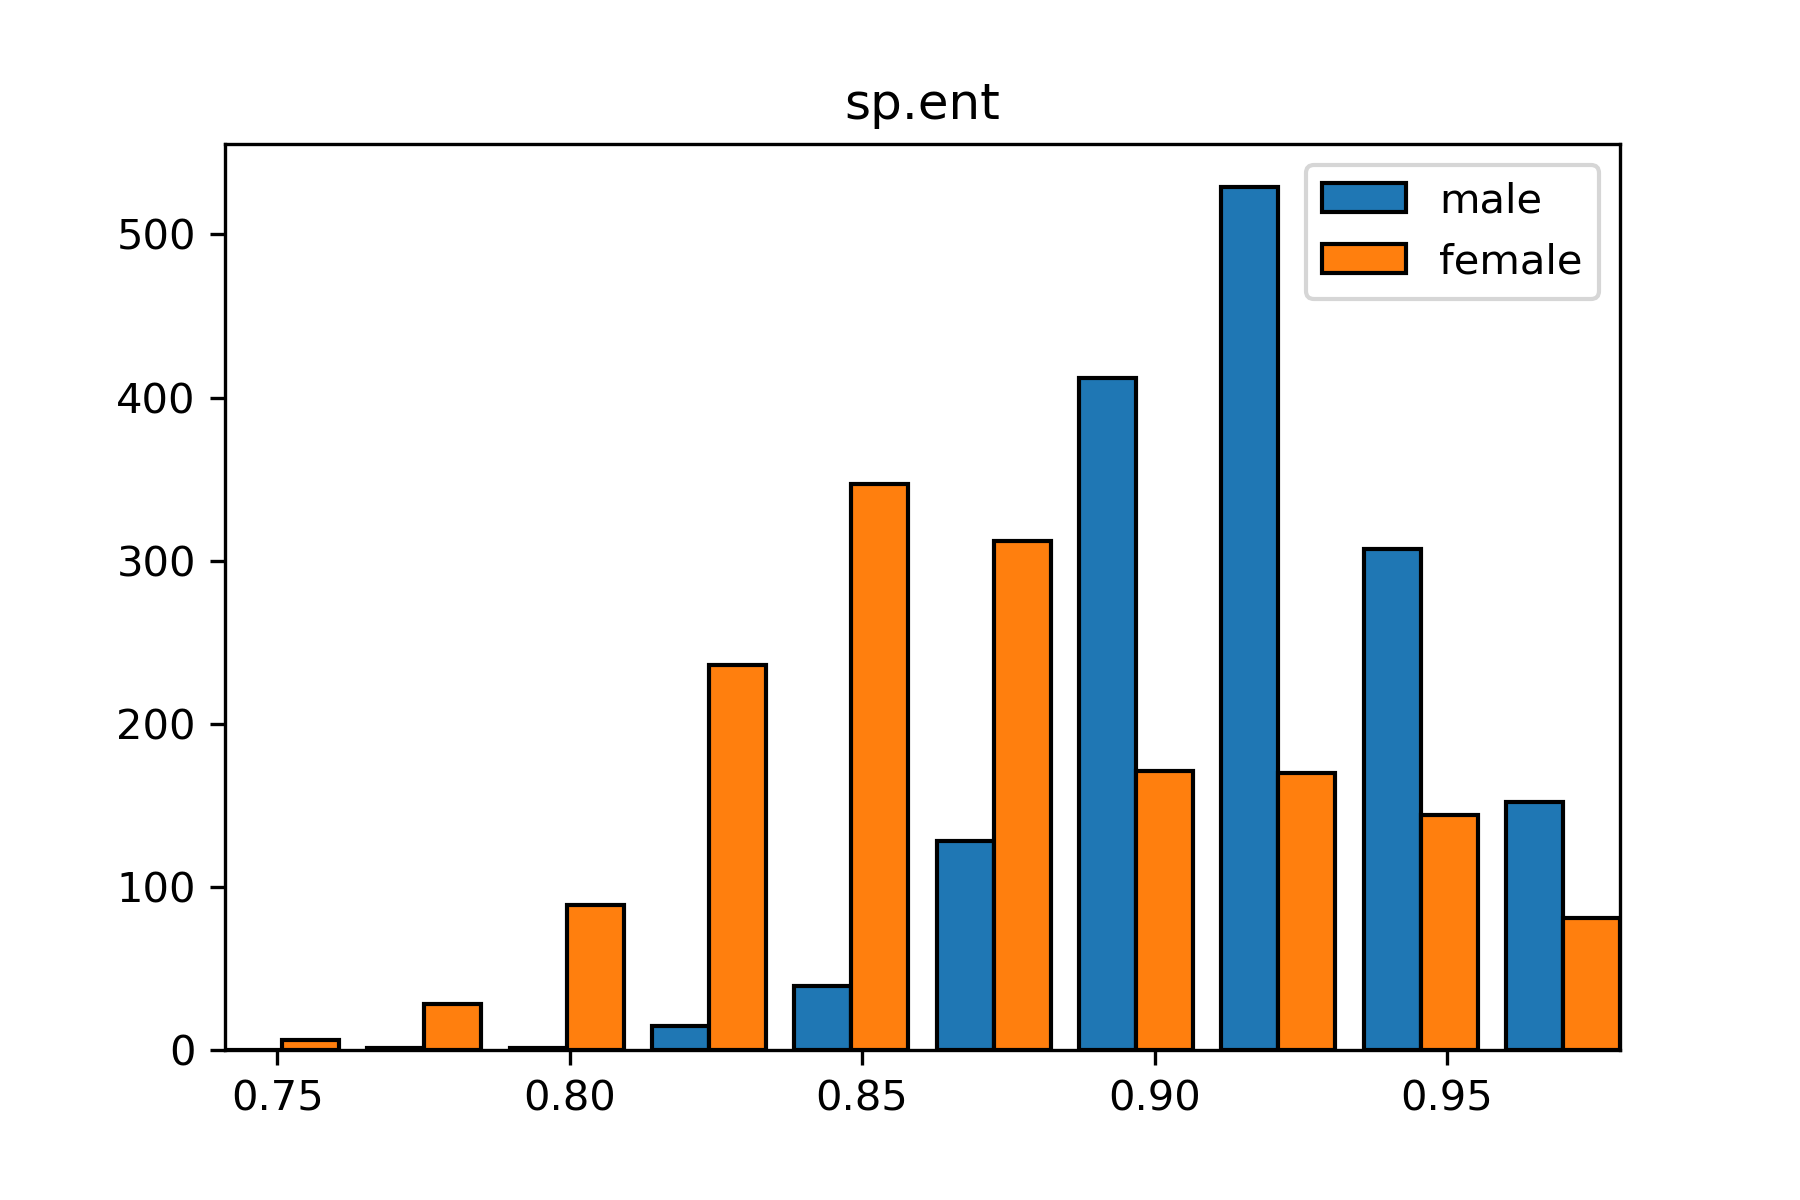
\includegraphics[width=3.85cm]{sbs_7_sp_ent}
        \caption{sp ent}
        \label{fig:sub_sbs_8}
    \end{subfigure}\hfill
    % sfm
    \begin{subfigure}{0.32\textwidth}
        \centering
        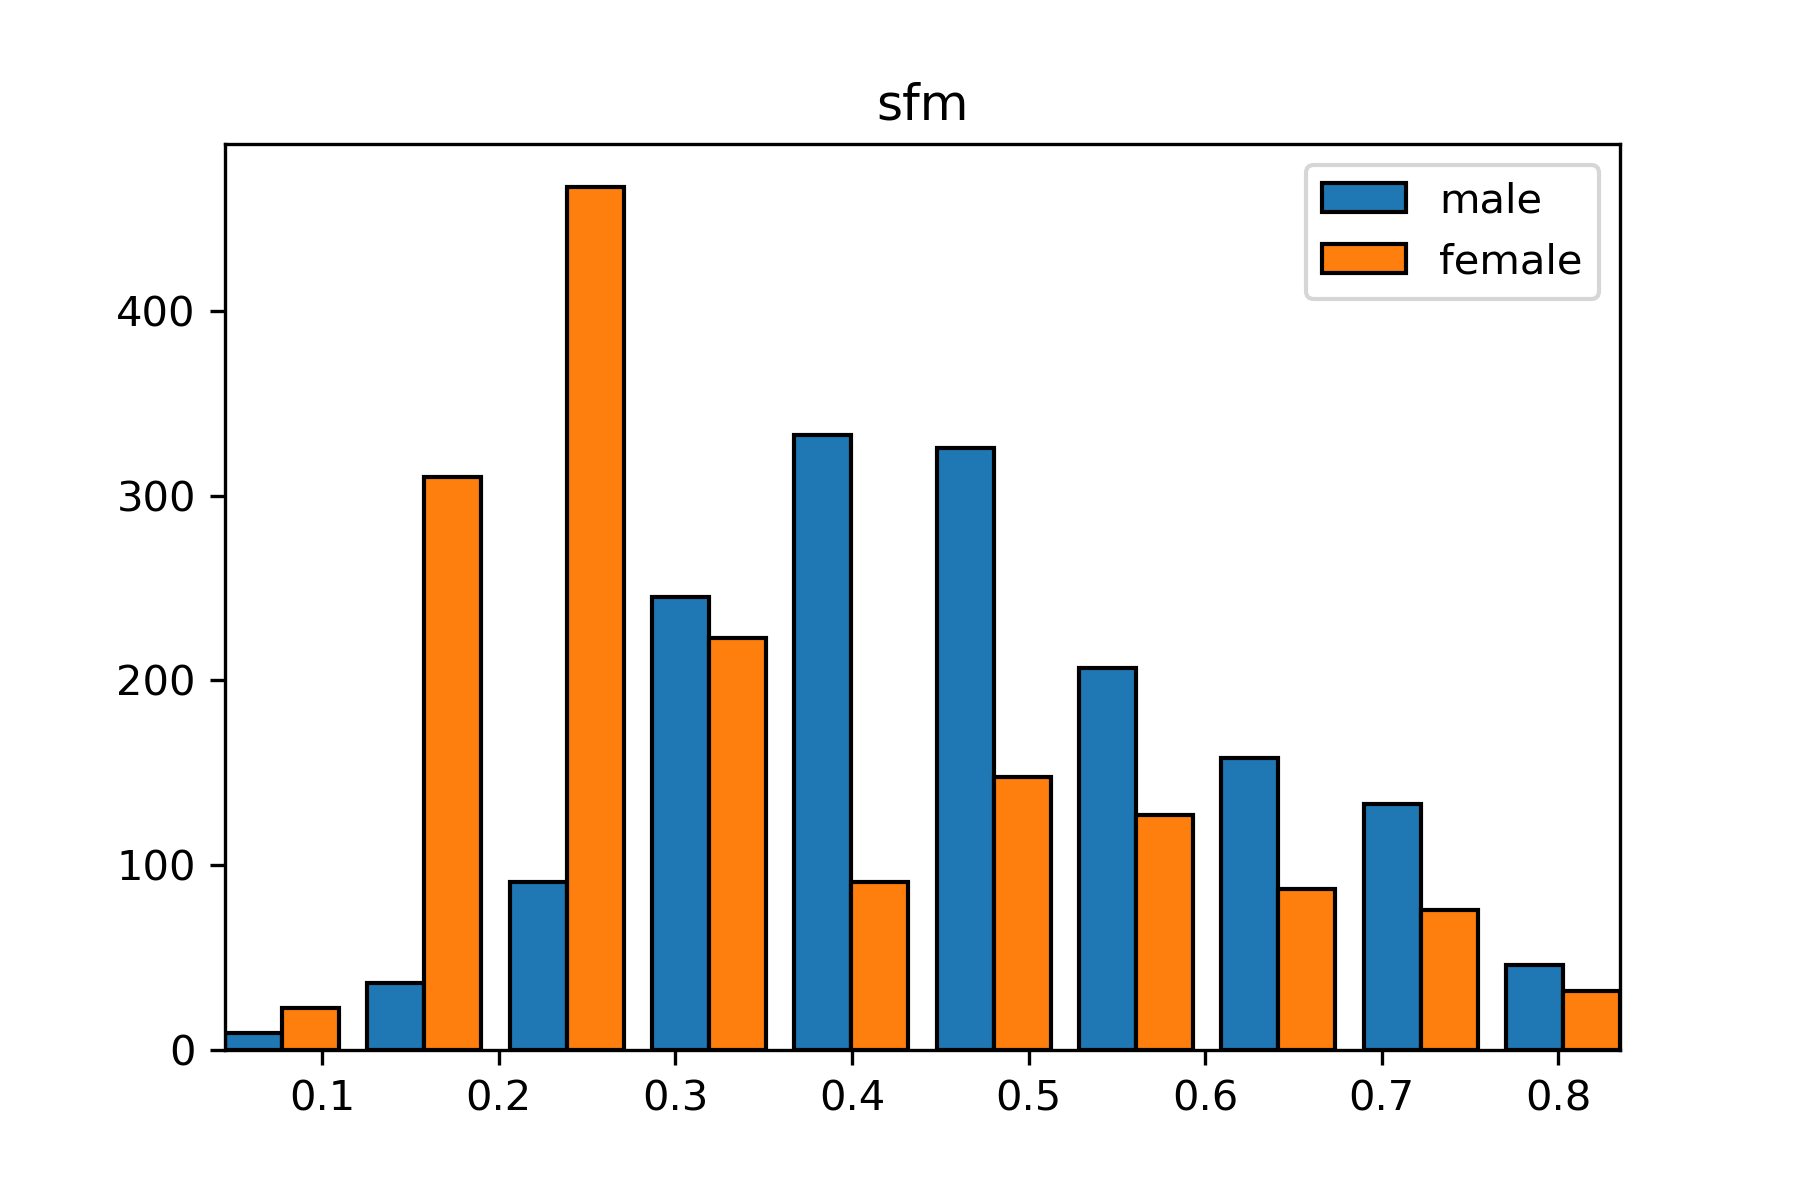
\includegraphics[width=3.85cm]{sbs_8_sfm}
        \caption{smf}
        \label{fig:sub_sbs_9}
    \end{subfigure}\hfill
    % mode
    \begin{subfigure}{0.32\textwidth}
        \centering
        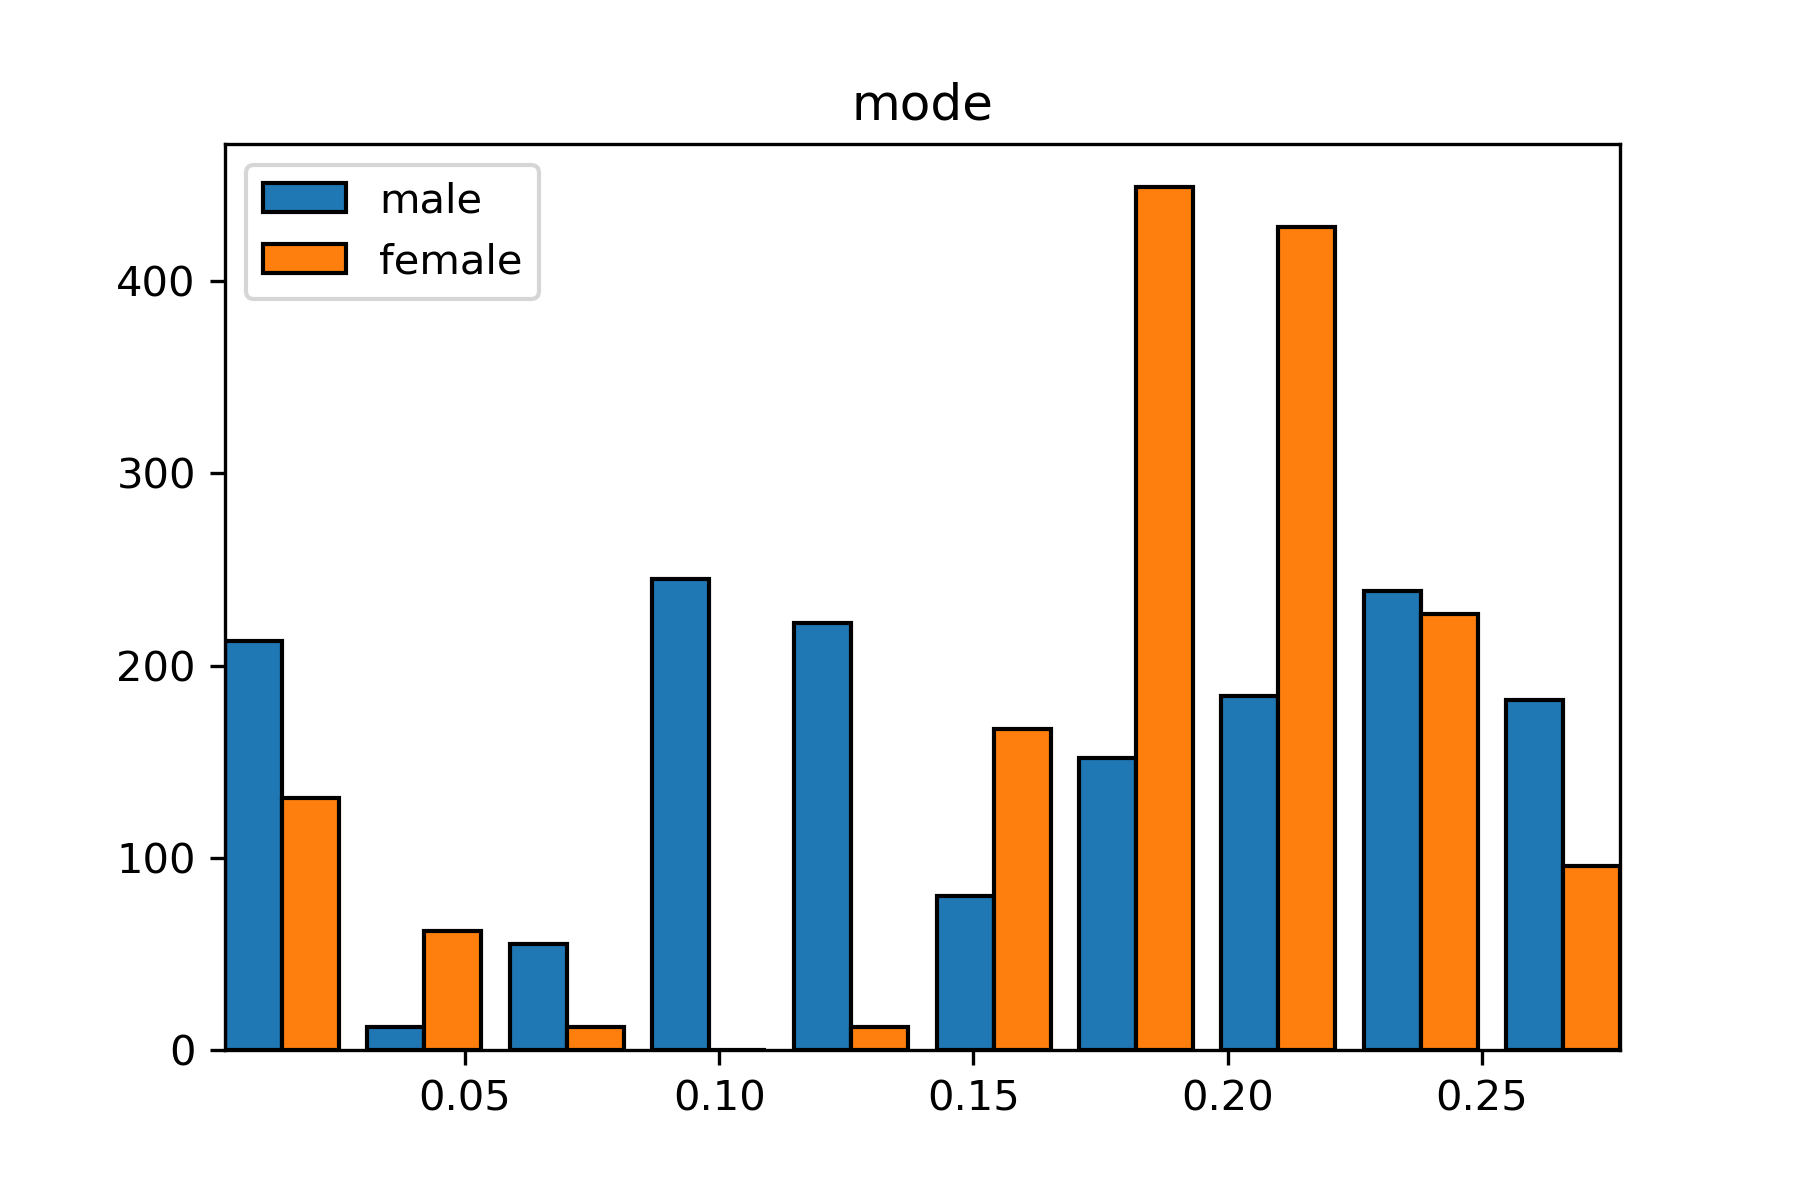
\includegraphics[width=3.85cm]{sbs_9_mode}
        \caption{mode}
        \label{fig:sub_sbs_10}
    \end{subfigure}\hfill
    % centroid
    \begin{subfigure}{0.32\textwidth}
        \centering
        \includegraphics[width=3.85cm]{sbs_10_centroid}
        \caption{centroid}
        \label{fig:sub_sbs_11}
    \end{subfigure}\hfill
    % meanfun
    \begin{subfigure}{0.32\textwidth}
        \centering
        \includegraphics[width=3.85cm]{sbs_11_meanfun}
        \caption{meanfun}
        \label{fig:sub_sbs_12}
    \end{subfigure}\hfill
    % minfun
    \begin{subfigure}{0.32\textwidth}
        \centering
        \includegraphics[width=3.85cm]{sbs_12_minfun}
        \caption{minfun}
        \label{fig:sub_sbs_13}
    \end{subfigure}\hfill
    % maxfun
    \begin{subfigure}{0.32\textwidth}
        \centering
        \includegraphics[width=3.85cm]{sbs_13_maxfun}
        \caption{maxfun}
        \label{fig:sub_sbs_14}
    \end{subfigure}\hfill
    % meandom
    \begin{subfigure}{0.32\textwidth}
        \centering
        \includegraphics[width=3.85cm]{sbs_14_meandom}
        \caption{meandom}
        \label{fig:sub_sbs_15}
    \end{subfigure}\hfill
    % mindom
    \begin{subfigure}{0.32\textwidth}
        \centering
        \includegraphics[width=3.85cm]{sbs_15_mindom}
        \caption{mindom}
        \label{fig:sub_sbs_16}
    \end{subfigure}\hfill
    % maxdom
    \begin{subfigure}{0.32\textwidth}
        \centering
        \includegraphics[width=3.85cm]{sbs_16_maxdom}
        \caption{maxdom}
        \label{fig:sub_sbs_17}
    \end{subfigure}\hfill
    % dfrange
    \begin{subfigure}{0.32\textwidth}
        \centering
        \includegraphics[width=3.85cm]{sbs_17_dfrange}
        \caption{dfrange}
        \label{fig:sub_sbs_18}
    \end{subfigure}\hfill
    % modindx
    \begin{subfigure}{0.32\textwidth}
        \centering
        \includegraphics[width=3.85cm]{sbs_18_modindx}
        \caption{modindx}
        \label{fig:sub_sbs_19}
    \end{subfigure}
    % caption and label
    \caption{Histograms of input features after data standardization}
    \label{fig:pre-ex1-sbs_histograms}
\end{figure}

\paragraph{In the Figure \ref{fig:pre-ex1-correlation} we can see the correlation matrix, with values between 0 and 1, mapped in colors. We can see from this image, that there are cases where a feature is highly correlated to another and also cases in which no significative correlation was measured. For example, features like ``skew'' and ``kurt'', ``maxdom'' and ``dfrange'', ``centroid'', ``Q25'' and ``median'' have a high correlation. In fact, if we look into these two first pairs of features, we can see that the shape of the histograms are very similar.}

\paragraph{On the other hand, features like ``sd'' and ``Q25'', ``IQR'' and Q25, ``centroid'' and ``sfm'', presents a low correlation. An intuition about this can be inferred from the fact that for all these pair of features, the shape of the plots in the histograms are kind of mirrored. For example, for the ``IQR'' feature the orange data is plotted before the blue data, while in ``Q25'' the opposite happens. One thing to be noted is that the matrix presents a symmetry with respect to the diagonal of this matrix, indicating that the correlation of A with respect to B is the same of the correlation of B with respect to A.}

\begin{figure}[H]
%    \centering
    \includegraphics[width=15cm]{correlation}
    \caption{Correlation between input features}
    \label{fig:pre-ex1-correlation}
\end{figure}

\paragraph{In the first notebook we also plotted the logistic function, used in the model proposed for binary classification. The Figure \ref{fig:pre-ex1-logistic} shows the logistic function in an interval of -2 and 2.}

\begin{figure}[H]
    \centering
    \includegraphics[width=12cm]{logistic_function}
    \caption{Logistic function}
    \label{fig:pre-ex1-logistic}
\end{figure}

\paragraph{Before actually starting the binary classification proposed in exercise 1, one fact can be noted when comparing the logistic function (used in this exercise) and the non-linear function (hyperbolic tangent) used to transform the data in the exercise 2 of the previous list of exercises EFC1. The shape of these functions are very similar. Just to visualize the shape of the functions, the two functions are plotted in the same Figure \ref{fig:pre-ex1-logistic_tanh}. Here, the logistic function was multiplied by two, and subtracted by one in order to show the similar shape with the hyperbolic tangent (but with a different scale).}

\begin{figure}[H]
    \centering
    \includegraphics[width=12cm]{logistic_vs_tanh}
    \caption{Comparasion between hyperbolic tangent and logistic function (scaled and with offset)}
    \label{fig:pre-ex1-logistic_tanh}
\end{figure}

%=======================================
\subsection{b) Logistic regression, ROC and F1-score curves.}
%=======================================

\paragraph{In this subsection the binary classifier is actually coded. Here we are using the \textit{shuffle} function provided by the scikit-learn library. First, we separate the data according to the label. We do this to ensure that we have the same rate of both classes in the training set and also in the test set. The data in both groups are then shuffled.}

\paragraph{The training step is performed until the difference between successive iteration errors is under a provided tolerance. RMSE was chosen to be the error criteria. We are using a tolerance of $1.10^{-6}$, which means that when the error between the real and the predicted class for a iteration is less than the error in the previous iteration minus this tolerance, we should stop the training process. The error progression with the number of epochs is shown in Figure \ref{fig:ex1-error}. We are considering the whole batch of samples for each step during the training.}

\begin{figure}[H]
    \centering
    \includegraphics[width=12cm]{error}
    \caption{Error progression in training}
    \label{fig:ex1-error}
\end{figure}

\paragraph{Now we are going to plot the receiver operating characteristic (ROC) curve and the F1-score for the classifier. For this, we are using the metrics provided by the scikit-learn library. The ROC curve is plotted with the recall (true positive rate, tpr) being the y axis and the false positive rate (fpr) being the x axis. The ROC curve can be seen in the Figure \ref{fig:ex1-roc}. We can see that the ROC curve is located at a high part of the graph as well it is to the left, indicating a good performance.}

\begin{figure}[H]
    \centering
    \includegraphics[width=12cm]{ROC}
    \caption{ROC curve}
    \label{fig:ex1-roc}
\end{figure}

\paragraph{We now change the threshold used to classify a sample with the positive or negative class. We used values of threshold from 0 to 1 with step of 0.001, i.e., we are using 1000 different thresholds values. For each value of threshold we calculated the F1-score. Figure \ref{fig:ex1-f1_score} shows this plot.}

\begin{figure}[H]
    \centering
    \includegraphics[width=12cm]{F1_score}
    \caption{F1-score curve}
    \label{fig:ex1-f1_score}
\end{figure}

%=======================================
\subsection{c) Threshold, confusion matrix and accuracy.}
%=======================================

\paragraph{If we give a zoom in Figure \ref{fig:ex1-f1_score} highlighting the points near the maximum of the curve, as shown in Figure \ref{fig:ex1-f1_score_zoom}, we can choose the most appropriate threshold value. Knowing that the F1-score can be interpreted as a weighted average of the precision and recall (with 1 being the best value and 0 being the worst), we then choose for the threshold which maximizes the F1-score. This gives us a threshold of 0.689.}

\begin{figure}[H]
    \centering
    \includegraphics[width=12cm]{F1_score_zoom}
    \caption{Zoom in F1-score curve}
    \label{fig:ex1-f1_score_zoom}
\end{figure}
\newpage

\paragraph{Using the chosen threshold (with value 0.689) we now plot the confusion matrix. The Figure \ref{fig:ex1-cm_raw} shows the confusion matrix with raw values and the Figure \ref{fig:ex1-cm_norm} shows the one with normalized values.}

\begin{figure}[H]
    \centering
    \includegraphics[width=12cm]{binary_cm_raw}
    \caption{Confusion Matrix for binary classification (logistic regression)}
    \label{fig:ex1-cm_raw}
\end{figure}

\begin{figure}[H]
    \centering
    \includegraphics[width=12cm]{binary_cm_norm}
    \caption{Confusion Matrix normalized for binary classification (logistic regression)}
    \label{fig:ex1-cm_norm}
\end{figure}

\paragraph{Finally, we can calculate the accuracy for this classifier, which gives us a value of 0.9826, indicating a good performance.}

%=================================================
\section{Part 2 - Multiclass Classification}
%=================================================

\paragraph{We start this exercise by performing a one-hot encoding with the data. This way we can represent the categorical variables in a binary way. This encoding is defined as follows:}

\medskip
\begin{center}
    \begin{minipage}{.4\textwidth}
        \underline{\textbf{output:}}\medskip\\
        1 – caminhada\\
        2 – subindo escadas\\
        3 – descendo escadas\\
        4 – sentado\\
        5 – em pé\\
        6 – deitado\\[3mm]
        \underline{\textbf{one-hot enconding:}}\medskip\\
        $[$1 0 0 0 0 0$]^T$: walking\\
        $[$0 1 0 0 0 0$]^T$: climbing stairs\\
        $[$0 0 1 0 0 0$]^T$: going down stairs\\
        $[$0 0 0 1 0 0$]^T$: seated\\
        $[$0 0 0 0 1 0$]^T$: standing\\
        $[$0 0 0 0 0 1$]^T$: lying
    \end{minipage}
\end{center}

%=======================================
\subsection{a) Logistic regression (using softmax approach)}
%=======================================

\paragraph{The approach used to implement the multiclass classifier was the softmax function. All operations involved was performed in the matrix way, in order to try to improve the computational costs involved.}

\paragraph{A weight array with K+1 elements (in this case we have K = 561 features) is randomly initiated according to a uniform distribution between -1 and 1 for each class, as can be seen:}

\[ \boldsymbol{w_C} = \begin{bmatrix} w_0^{(C)} & w_1^{(C)} & ... & w_K^{(C)} \end{bmatrix}^T \]

\paragraph{As we have six different classes, the W matrix can be generated as follows:}

\[ \boldsymbol{W} = \begin{bmatrix} \boldsymbol{w_0} & \boldsymbol{w_1} & ... & \boldsymbol{w_K} \end{bmatrix} = \begin{bmatrix} 
    w_0^{(0)} & w_0^{(1)} &   ...  & w_0^{(C)} \\ 
    w_1^{(0)} & w_1^{(1)} &   ...  & w_1^{(C)} \\
      \vdots  &   \vdots  & \ddots &   \vdots  \\
    w_K^{(0)} & w_K^{(1)} &   ...  & w_K^{(C)} \\
\end{bmatrix} \]

\paragraph{The stop criteria adopted was a tolerance of $2.10^{-2}$ for the error in a given iteration. The function used to calculate the error was the zero-one loss, where a 0 is assigned when the class was correctly classified, and 1 when it was not. We then calculate the zero-one loss for all data in the training set, sum all of them and divide by the number of inputs (7352 in this case).}

\paragraph{The variation of the error with the number of epochs is shown in the Figure \ref{fig:ex2-a-zero_one_loss}.}

\begin{figure}[H]
    \centering
    \includegraphics[width=12cm]{zero_one_loss}
    \caption{Zero-one loss curve}
    \label{fig:ex2-a-zero_one_loss}
\end{figure}

\paragraph{In the Figure \ref{fig:ex2-a-zero_one_loss_zoom} we can see a zoom of the previous curve focusing in the beginning of the curve. As we can see, the initial error is very high (bigger than 0.9) due to the randomly generated weights.}

\begin{figure}[H]
    \centering
    \includegraphics[width=12cm]{zero_one_loss_zoom}
    \caption{Zoom in zero-one loss curve}
    \label{fig:ex2-a-zero_one_loss_zoom}
\end{figure}

\paragraph{Now it is time to measure the performance of the classifier. To plot the confusion matrix we are using the ``\textit{plot\_confusion\_matrix}'' described in the notebook, and the ``\textit{f1\_score}'' function provided by the scikit-learn library.}

\paragraph{Figures \ref{fig:ex2-a-cm_raw} and \ref{fig:ex2-a-cm_norm} shows the confusion matrix with raw and normalized values, respectively.}

\begin{figure}[H]
    \centering
    \includegraphics[width=11cm]{cm_raw}
    \caption{Confusion Matrix using softmax model}
    \label{fig:ex2-a-cm_raw}
\end{figure}

\begin{figure}[H]
    \centering
    \includegraphics[width=11cm]{cm_norm}
    \caption{Confusion Matrix with normalized values using softmax model}
    \label{fig:ex2-a-cm_norm}
\end{figure}

\paragraph{Having the confusion matrix, we can calculate metrics to measure the performance of the classifier and compare with the k-Nearest Neighbor, the next model we will validate. The zero-one loss and the F1-score obtained are:}

\begin{itemize}
    \item Zero-one loss = 0.0929
    \item F1-score micro = 0.9080
    \item F1-score macro = 0.9071
\end{itemize}


%=======================================
\subsection{b) k-Nearest Neighbors}
%=======================================

\paragraph{For the k-Nearest Neighbors (kNN) method, we use a lazy learning method. For this, the first thing we should do is to calculate somehow the distance between the new data and all the data from the training set. The distance metric used here was the Minkowski.}

\paragraph{Minkowski distance:}

\[ d(x,y) = \left( \sum_{i=1}^{K} |x_i - y_i|^p \right)^{1/p} \]

\paragraph{For \textit{p = 2}, we have the Euclidian distance:}

\[ d(x,y) = \sqrt{\sum_{i=1}^{K} |x_i - y_i|^2} \]

\paragraph{In order to reduce the calculation costs, the distance between all data from the training set and all data in the validation set were calculated in the matrix form. A distance matrix $D$ was created for this, as can be seen as follows:}

\begin{center}
\textit{D}: distances matrix\\
\textit{D} shape: (M x N)
\end{center}

\begin{center}
    \begin{minipage}{.7\textwidth}
        \[ D = \begin{bmatrix}
          d(x_{T_0},x_{D_0}) & d(x_{T_0},x_{D_1}) &   ...  & d(x_{T_0},x_{D_N}) \\ 
          d(x_{T_1},x_{D_0}) & d(x_{T_1},x_{D_1}) &   ...  & d(x_{T_1},x_{D_N}) \\ 
                 \vdots      &       \vdots       & \ddots &        \vdots      \\
          d(x_{T_M},x_{D_0}) & d(x_{T_M},x_{D_1}) &   ...  & d(x_{T_M},x_{D_N}) \\ 
        \end{bmatrix} \]
        Where:
        \begin{itemize}
            \item $x_{T_M}$ is the M$^{th}$ sample of training set
            \item $x_{D_N}$ is the N$^{th}$ sample of data set
            \item $d(x_{T_M},x_{D_N})$ is the Minkowski distance between the points $x_{T_M}$ and $x_{D_N}$
        \end{itemize}
    \end{minipage}
\end{center}

%=======================================

\subsubsection{Uniform weights}

\paragraph{During the decision step two approaches were used. The first one presented here uses uniform weights, i.e., each k neighbors have the same weight when voting for their own class. The result for this approach can be seen in the Figure \ref{fig:ex2-b-error_uniform}. In Figure \ref{fig:ex2-b-error_uniform_zoom} we can see a zoom in the previous plot showing the value of k optimum = 5, which minimizes the loss function.}

\begin{figure}[H]
    \centering
    \includegraphics[width=12cm]{error_uniform}
    \caption{Zero-one loss curve (uniform weights)}
    \label{fig:ex2-b-error_uniform}
\end{figure}

\begin{figure}[H]
    \centering
    \includegraphics[width=12cm]{error_uniform_(zoom)}
    \caption{Zero-one loss curve (uniform weights)}
    \label{fig:ex2-b-error_uniform_zoom}
\end{figure}

\paragraph{After finding the best value for the hyperparameter k = 5, we now apply the model to the test data. The results can be seen in Figures \ref{fig:ex2-b-cm_uniform} and \ref{fig:ex2-b-cm_uniform_normalized}, which shows the confusion matrix with raw values and with normalized values, respectively.}

\begin{figure}[H]
    \centering
    \includegraphics[width=12cm]{cm_uniform}
    \caption{Confusion Matrix for uniform weights}
    \label{fig:ex2-b-cm_uniform}
\end{figure}

\begin{figure}[H]
    \centering
    \includegraphics[width=12cm]{cm_uniform_normalized}
    \caption{Confusion Matrix normalized for uniform weights}
    \label{fig:ex2-b-cm_uniform_normalized}
\end{figure}

\paragraph{We then use metrics to measure the performance of the classifier. The results obtained are:}

\begin{itemize}
    \item Zero-one loss = 0.1274
    \item F1-score micro = 0.8592
    \item F1-score macro = 0.8557
\end{itemize}

%=======================================

\subsubsection{Distance weights}

\paragraph{The second approach uses distance weights. In this case, each vote is pondered according to the inverse of the distance. This means that when predicting the class for a new input, the class of a very similar data in the training set has more relevance than a data not so close to this new input. The result for this approach can be seen in the Figure \ref{fig:ex2-b-error_distance}. In Figure \ref{fig:ex2-b-error_distance_zoom} we can see a zoom in the previous plot showing the value of k optimum = 6, which minimizes the loss function.}

\begin{figure}[H]
    \centering
    \includegraphics[width=12cm]{error_distance}
    \caption{Zero-one loss curve (inversely proportional to distance weights}
    \label{fig:ex2-b-error_distance}
\end{figure}

\begin{figure}[H]
    \centering
    \includegraphics[width=12cm]{error_distance_(zoom)}
    \caption{Zero-one loss curve (inversely proportional to distance weights}
    \label{fig:ex2-b-error_distance_zoom}
\end{figure}

\paragraph{After finding the best value for the hyperparameter k = 6, we now apply the model to the test data. The results can be seen in Figures \ref{fig:ex2-b-cm_distance} and \ref{fig:ex2-b-cm_distance_normalized}, which shows the confusion matrix with raw values and with normalized values, respectively.}

\begin{figure}[H]
    \centering
    \includegraphics[width=11cm]{cm_distance}
    \caption{Confusion Matrix for uniform weights}
    \label{fig:ex2-b-cm_distance}
\end{figure}

\begin{figure}[H]
    \centering
    \includegraphics[width=11cm]{cm_distance_normalized}
    \caption{Confusion Matrix for distance weights}
    \label{fig:ex2-b-cm_distance_normalized}
\end{figure}

\paragraph{The last thing we did was to use metrics to measure the performance of the classifier. The results obtained are:}

\begin{itemize}
    \item Zero-one loss = 0.1030
    \item F1-score micro = 0.8816
    \item F1-score macro = 0.8787
\end{itemize}

%=======================================
\subsection{Results and conclusion}
%=======================================

\paragraph{We now can compare the performance between the two models proposed in a multiclass classification scenario. For the k-Nearest Neighbors, two approaches were used: one considering uniform weights for the neighbors and another one considering distance weights. Table \ref{tab:results} shows a summary of the results obtained:}

\begin{table}[H]
    \begin{center}
        \begin{tabular}{ r|c|c|c|} 
            \cline{2-4}
            \multicolumn{1}{r}{}
             & \multicolumn{1}{|c|}{softmax}
             & \multicolumn{2}{|c|}{kNN} \\
            \cline{3-4}
            & & distance & uniform \\
            \cline{2-4}
%            \multirow{2}{4em}{zero-one loss}& cell4 & cell5 & cell6 \\
            Zero-one loss   & 0.0920 & 0.1030 & 0.1274 \\
            F1-score: micro & 0.9080 & 0.8816 & 0.8592 \\
            F1-score: macro & 0.9071 & 0.8787 & 0.8557 \\
            \cline{2-4}
        \end{tabular}
    \end{center}
    \caption{Comparison of results between softmax and kNN models for multiclass classification}
    \label{tab:results}
\end{table}

\paragraph{As expected, the softmax model is more robust. It presents the smallest error and the highest value for the F1-score, both micro and micro, showing that the overall classification is good (macro) and also the classification in each individual class (micro).}

\paragraph{The kNN model, however, it does not present bad results when comparing to the softmax model. Actually, the results are quite reasonable, close to the ones obtained with the softmax function, which indicates that depending on the dataset and the problem, it can be an easy to implement and low cost alternative, considering that there is no training in this method, but only distance measures and comparison between them.}

\paragraph{Still talking about the kNN model, when comparing the two approaches used, the distance weights has a superior performance than the uniform weights, even though the number of neighbors used are similar (5 for the uniform approach and 6 for the distance approach, chose by a cross-validation method).}

%=================================================
\end{document}
